\documentclass[a4paper,10pt]{book}
\usepackage{lmodern}
\usepackage[utf8]{inputenc}
\usepackage[english]{babel}
\usepackage[pdfborder={0 0 0}]{hyperref} % Hyperlinks
\usepackage{xcolor}
\usepackage{amsmath}
\usepackage{graphicx}
\usepackage{longtable}
\usepackage{array}
\usepackage{hyphsubst}
\usepackage[T1]{fontenc}
\usepackage{microtype}
\usepackage[parfill]{parskip} % Blank line between paragraphs
\usepackage[section]{placeins}
\usepackage{enumitem}
\newcommand*{\descrfont}[1]{\textit{#1 -}}
\newcommand{\icon}[1]{\includegraphics[height=2ex]{#1}}

%define languages for code examples
\usepackage{listings}
\definecolor{lightgray}{rgb}{0.97,0.97,0.97}
\lstdefinelanguage{XML}
{
  frame=single,
  morestring=[b]",
  morestring=[b]{"}{"},
  moredelim=[s][\color{orange}]{>}{<},
  morecomment=[s]{<?}{?>},
  morecomment=[s]{<!--}{-->},
  morekeywords={xmlns,version,type,soapenv,sync,data,map},
}
\lstdefinelanguage{Plain}
{
  numbers=none,
  keywords={}
  keywordstyle=\color{black},
  identifierstyle=\color{black},
  commentstyle=\color{black},
  stringstyle=\color{black},
}
\lstset{
  backgroundcolor=\color{lightgray},
  basicstyle=\ttfamily\color{black}\bfseries\small,
  captionpos=b,
  identifierstyle=\color{blue},
  keywordstyle=\color{cyan},
  language=XML,
  numbers=left,
  numbersep=5pt,
  numberstyle=\tiny,
  showstringspaces=false,
  stringstyle=\color{orange},
  tabsize=2,
}


\providecommand{\tightlist}{%
  \setlength{\itemsep}{0pt}\setlength{\parskip}{0pt}}

\newcommand*{\vnversion}{1.18}
\title{verinice User Guide \vnversion{}}
\author{SerNet GmbH}

% Header and footer setup
\usepackage{fancyhdr}
\fancyhf{} % Empty header and footer
\fancyfoot[C]{\small \copyright{} \the\year\ SerNet GmbH} % Set footer
\renewcommand{\headrulewidth}{1pt} % Set dividing line for header
\renewcommand{\footrulewidth}{1pt} % Set divide line for footer
\fancypagestyle{plain}{} % Set fancy stlye for "plain" pages
\pagestyle{fancy} % Set fancy page style

\setlength{\parindent}{0pt}

\fancyfoot[OL,ER]{\thepage} % Odd page numbers left, even pages number right
\fancyhead[RE,LO]{\leftmark}

\hyphenation{}

% Prevent orphans and widows (https://en.wikipedia.org/wiki/Widows_and_orphans)
\clubpenalty=10000
\widowpenalty=10000
\displaywidowpenalty=10000


\begin{document}

\pagenumbering{roman}

\begin{titlepage}
    \centering
    \vspace{1cm}
    \begin{figure}[htb!]
      \centering
      \colorbox{white}{
\includegraphics{Image/logo.pdf}}
    \end{figure}
    \huge\textbf{User Guide \vnversion{}}\\
    \vspace{14cm}
    \normalsize
  \copyright{} \the\year\ SerNet GmbH\\
  Any kind of copies, even in extracts, are only allowed with the\\
  authorization of SerNet GmbH.\\
  Exclusive sale by SerNet GmbH, Bahnhofsallee 1b, 37081 Göttingen, Germany.
\end{titlepage}

\tableofcontents

\listoftables

\listoffigures

\chapter{Introduction}
\pagenumbering{arabic}
Thank you for deciding to use verinice.

Verinice is a tool for managing information security, complying with standards,
laws, and regulations, and a tool that will accompany you through information
security audits. Typical verinice users include: Information security officers,
data security officers, administrators, internal and external auditors,
SO 27001 auditors, security auditors, process owners, or chief executive
officers.

For ease of readability, in this manual the masculine form is always used -
nevertheless female and male readers are addressed.

This manual describes verinice \vnversion{}.

\newpage
\chapter{Installation and configuration}
\section{verinice client}
\subsection{System requirements}
The following operating system requirements must be met for optimum use of
verinice:

\begin{itemize}
  \item Windows 7, Windows 10

    verinice also runs on any other versions of Microsoft Windows. However, verinice
    is not tested by SerNet on these versions.

  \item macOS 10.14 Mojave

    verinice also runs on other versions of macOS. However, verinice is not tested
    by SerNet on these versions.

  \item Linux
    \begin{itemize}
      \item Ubuntu 18.04.x LTS
      \item Ubuntu 16.04.x LTS
      \item CentOS 7.x
      \item Red Hat Enterprise Linux 7.x
    \end{itemize}

    verinice also runs on other Linux distributions and versions.
    However, that's not tested extensively by SerNet.
\end{itemize}

\subsection{Installation and update}
\label{sec:installation} %foo
On the \href{http://verinice.org/\#download}{www.verinice.org/\#download}
website, select the verinice download that matches your platform. verinice is
provided as a zip or tgz formatted archive. There is no need to install;
verinice starts from the folder in which the downloaded archive file is
extracted. The user's data is stored by default in the "verinice" folder in
the user's home directory; this folder is automatically generated for this
purpose.

The location of the user's home folder depends on the operating system. The
following cases are the defaults:

\colorbox{lightgray}{\parbox{\textwidth}{
\begin{itemize}
  {\em
    \item on Windows 7: C:\textbackslash user\textbackslash\textless
      username\textgreater
    \item on Linux: /home/\textless username\textgreater
  }
\end{itemize}
}}

The operating system user needs write permission on the verinice folder to
perform updates. Otherwise, the update function must be launched via the
account that unpacked the archive. Use of verinice is still possible
despite this. This is especially true if verinice is installed in
{\em C:\textbackslash Programs} on a Windows computer. Updates in this folder
can only be performed by a user with administrator permissions.

Credentials to update a client are available at \url{http://v.de/client-shop}.

After unpacking, verinice is ready for use and can be launched. You can do
this, e.g., by double clicking the verinice application file. When you first
launch verinice, a welcome screen appears, providing a brief overview of the
application's options. Select one of the following starting perspectives:
\begin{itemize}
  \item ISM
  \item BSI IT baseline security
  \item Information Security Assessment (ISA)
\end{itemize}
In the default configuration, you will now see the application with a catalog
window (on the left), an inventory panel (at the center), and a tutorial
window (on the right) (see figure \ref{Standard configuration of verinice}).
\begin{figure}[htb!]
  \centering
  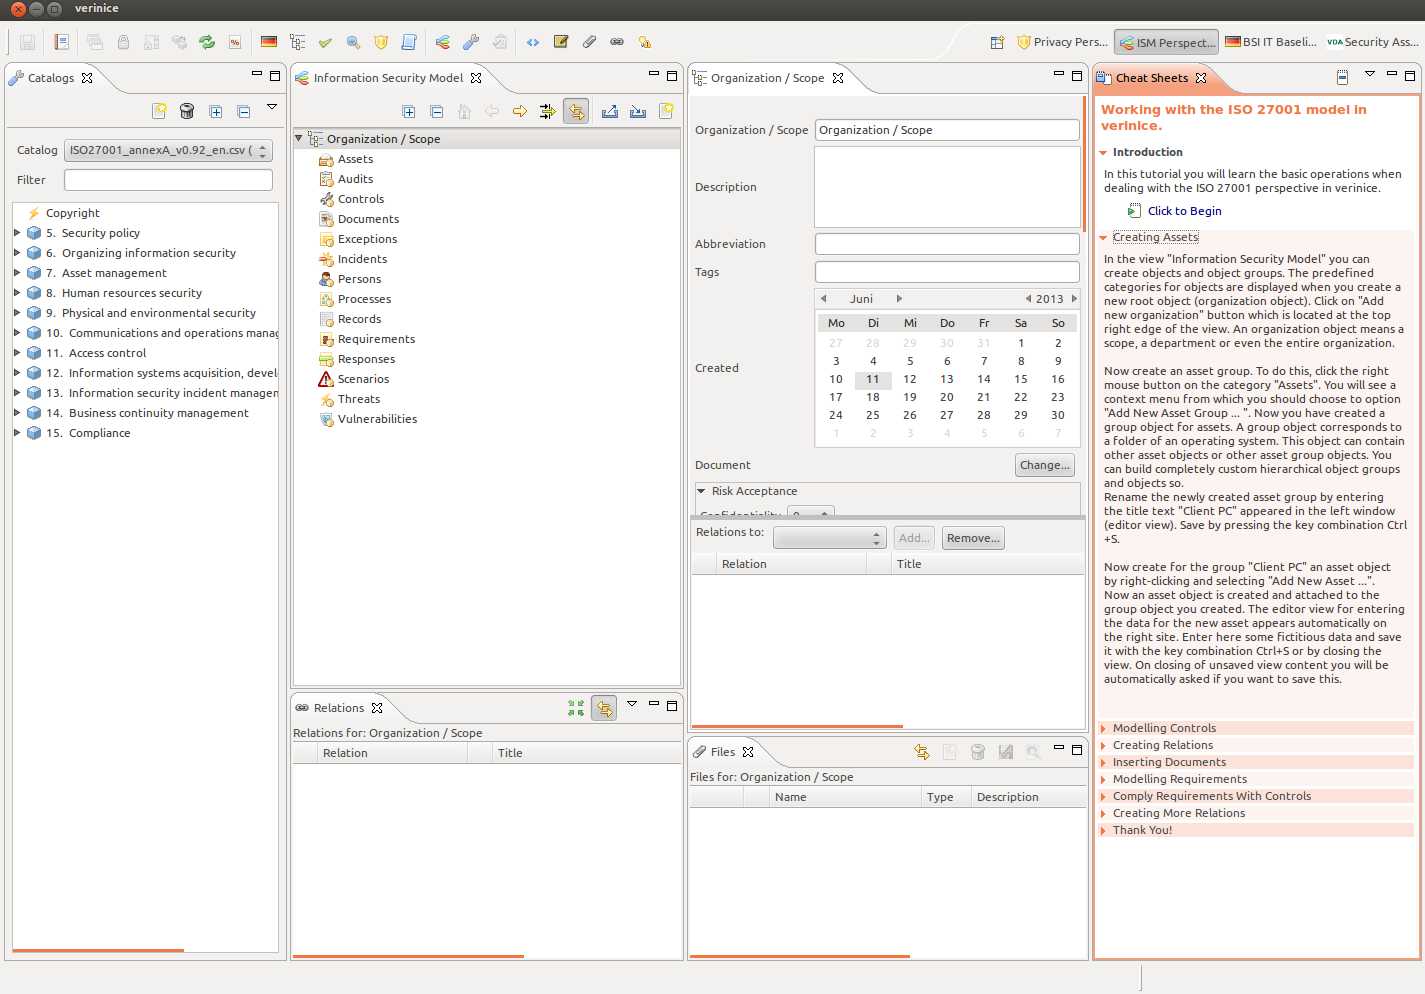
\includegraphics[scale=.24]{Screenshot/ISM-Perspektive-en.png}
  \caption{
    \label{Standard configuration of verinice} Standard configuration
      of verinice
  }
\end{figure}

\subsection{Licensing}
verinice is a free program released under the GPLv3 License
\href{http://www.gnu.org/licenses/gpl-3.0.txt}{\em GPLv3}\footnote{\url{http://www.gnu.org/licenses/gpl-3.0.html}}.
Components used by it are released under the {\em Apache License}\footnote{\url{http://www.apache.org/licenses/LICENSE-2.0}}
and the {\em Eclipse Public License}\footnote{\url{http://opensource.org/licenses/EPL-1.0}}.
The help menu provides an overview of the licenses for the individual plugins. You will find them in verinice under
\textbf{Help \textgreater About verinice}.

\subsection{Uninstalling}
To uninstall, please remove the folder in which verinice was unpacked and the verinice working directory
that was created from the operating system user's home directory.

\section{Installing the verinice.PRO server component}
Assuming you have the required subscription access credentials, you
can download the required installation instructions from
\url{https://update.verinice.com/pub/Manuals/}.

\chapter{Icons and keyboard shortcuts}
\section{Basic icons}
The basic icons are divided into four groups:
\newline\\
\textbf{General icons}
%\renewcommand{\arraystretch}{1.2}

\begin{longtable}{| c | p{0.8\textwidth} |}
\hline
\raisebox{-0.6\height}{\textbf{Icon}} & \raisebox{-0.6\height}{\textbf{Meaning}} \\[10pt]
\hline\hline
\raisebox{-0.6\height}{
\includegraphics{Icon/New_persp.png}} & \raisebox{-0.6\height}{{Perspective selection}} \\[10pt] \hline
\raisebox{-0.6\height}{
\includegraphics{Icon/Disk.png}} & \raisebox{-0.6\height}{Save} \\[10pt] \hline
\raisebox{-0.6\height}{
\includegraphics{Icon/Report.png}} & \raisebox{-0.6\height}{Generate report} \\[10pt] \hline
\raisebox{-0.6\height}{
\includegraphics{Icon/Masseneditor.png}} & \raisebox{-0.6\height}{Edit matching elements together} \\[10pt] \hline
\raisebox{-0.6\height}{
\includegraphics{Icon/Zugriffsrechte.png}} & \raisebox{-0.6\height}{Edit access permissions} \\[10pt] \hline
\raisebox{-0.6\height}{
\includegraphics{Icon/Berechtigungsprofile.png}} & \raisebox{-0.6\height}{Edit user profiles} \\[10pt] \hline
\raisebox{-0.6\height}{
\includegraphics{Icon/user_suit.png}} & \raisebox{-0.6\height}{Edit accounts} \\[10pt] \hline
\raisebox{-0.6\height}{
\includegraphics{Icon/user_add.png}} & \raisebox{-0.6\height}{Create new accounts} \\[10pt] \hline
\raisebox{-0.6\height}{
\includegraphics{Icon/user_disabled.png}} & \raisebox{-0.6\height}{Disable accounts} \\[10pt] \hline
\raisebox{-0.6\height}{
\includegraphics{Icon/group.png}} & \raisebox{-0.6\height}{Account groups} \\[10pt] \hline
\raisebox{-0.6\height}{
\includegraphics{Icon/group_add.png}} & \raisebox{-0.6\height}{Create new account groups} \\[10pt] \hline
\raisebox{-0.6\height}{
\includegraphics{Icon/group_edit.png}} & \raisebox{-0.6\height}{Edot account groups} \\[10pt] \hline
\raisebox{-0.6\height}{
\includegraphics{Icon/group_delete.png}} & \raisebox{-0.6\height}{Delete account groups} \\[10pt] \hline
\raisebox{-0.6\height}{
\includegraphics{Icon/folder_table.png}} & \raisebox{-0.6\height}{Report repository} \\[10pt] \hline
\raisebox{-0.6\height}{
\includegraphics{Icon/Aktualisieren.png}} & \raisebox{-0.6\height}{Refresh view} \\[10pt] \hline
\raisebox{-0.6\height}{
\includegraphics{Icon/Verinice_linked.png}} & \raisebox{-0.6\height}{Link to editor} \\[10pt] \hline
\raisebox{-0.6\height}{
\includegraphics{Icon/Baustein.png}} & \raisebox{-0.6\height}{Module/Control group (depending on your perspective)} \\[10pt] \hline
\raisebox{-0.6\height}{
\includegraphics{Icon/Massnahmenbrowser.png}} & \raisebox{-0.6\height}{Object browser} \\[10pt] \hline
\raisebox{-0.7\height}{
\includegraphics{Icon/Notizen.png}} & \raisebox{-0.7\height}{Notes} \\[10pt] \hline
\raisebox{-0.6\height}{
\includegraphics{Icon/Hinzufuegen.png}} & \raisebox{-0.6\height}{Files} \\[10pt] \hline
\raisebox{-0.6\height}{
\includegraphics{Icon/Relationen.png}} & \raisebox{-0.6\height}{Relations} \\[10pt] \hline
\raisebox{-0.6\height}{
\includegraphics{Icon/quickfix_warning_obj.png}} & \raisebox{-0.6\height}{Validation} \\[10pt] \hline
\raisebox{-0.6\height}{
\includegraphics{Icon/Unbearbeitet.png}} & \raisebox{-0.6\height}{Implementation status {\em unedited}} \\[10pt] \hline
\raisebox{-0.6\height}{
\includegraphics{Icon/Nein.png}} & \raisebox{-0.6\height}{Implementation status {\em No}} \\[10pt] \hline
\raisebox{-0.6\height}{
\includegraphics{Icon/Teilweise.png}} & \raisebox{-0.6\height}{Implementation status {\em partially}} \\[10pt] \hline
\raisebox{-0.6\height}{
\includegraphics{Icon/Okay.png}} & \raisebox{-0.6\height}{Implementation status {\em yes}} \\[10pt] \hline
\raisebox{-0.6\height}{
\includegraphics{Icon/Entbehrlich.png}} & \raisebox{-0.6\height}{Implementation status {\em not applicable}} \\[10pt] \hline
\raisebox{-0.6\height}{
\includegraphics[scale=5]{Icon/Alien.png}} & \raisebox{-0.6\height}{Imported but not naturalized object} \\[10pt] \hline
\raisebox{-1\height}{
\includegraphics{Icon/Oeffnen.png}} & \raisebox{-0.6\height}{\parbox{0.7\textwidth}{Import catalog / Add new organization \linebreak / Adding file}} \\[10pt] \hline
\raisebox{-0.6\height}{
\includegraphics{Icon/Verknuepfungen.png}} & \raisebox{-0.6\height}{Linking with elements} \\[10pt] \hline
\raisebox{-3.0\height}{$\leftarrow$ $\rightarrow$ $\downarrow$ $\uparrow$} & One of the four arrows replaces the previous icon and, in combination with the dark frame, shows you the new location of the view as soon as you leave the current view with the left mouse button pressed \\[10pt] \hline
\raisebox{-1.0\height}{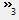
\includegraphics{Icon/Versteckte_Reiter.png}} & This icon appears if not all open tabs can be displayed in a view; the number behind the double-headed arrow shows the number of hidden tabs  \\[10pt] \hline
\raisebox{-1\height}{
\includegraphics{Icon/Filter.png}} & Filter settings allow you to select individual elements that you are searching for \\[10pt] \hline
\raisebox{-0.6\height}{
\includegraphics{Icon/Siegelstufe_A.png}} \raisebox{-0.6\height}{
\includegraphics{Icon/Siegelstufe_B.png}} \raisebox{-0.6\height}{
\includegraphics{Icon/Siegelstufe_C.png}} \raisebox{-0.6\height}{
\includegraphics{Icon/Siegelstufe_Z.png}} & \raisebox{-0.6\height}{Seal levels for controls (A, B, C, Z)} \\[10pt] \hline
\raisebox{-0.6\height}{
\includegraphics{Icon/Gefaehrdungen.png}} & \raisebox{-0.6\height}{Threats} \\[10pt] \hline
\raisebox{-1\height}{
\includegraphics{Icon/Ziel.png}} & Within the relations view, this takes you directly to the target for the selected link \\[10pt] \hline
\raisebox{-1.5\height}{
\includegraphics{Icon/Haengt_Ab.png}} & {\em Depends on} (a lower order component on the IT network was dragged and dropped into a higher order component during linking) \\[10pt] \hline
\raisebox{-1.5\height}{
\includegraphics{Icon/Noetig_Fuer.png}} & {\em Is necessary for} (a higher order component on the IT network was dragged and dropped into a lower order component during linking) \\[10pt] \hline
\raisebox{-0.6\height}{
\includegraphics{Icon/Verknuepfung_Aufheben.png}} & \raisebox{-0.6\height}{Unlink} \\[10pt] \hline
\raisebox{-0.6\height}{
\includegraphics{Icon/Export.png}} & {Export one or multiple organization/s, IT networks or security assessments} \\[10pt] \hline
\raisebox{-0.6\height}{
\includegraphics{Icon/Import.png}} & {Import one or multiple organization/s, IT networks or security assessments} \\[10pt] \hline
\raisebox{-0.6\height}{
\includegraphics{Icon/Nav_home.png}} & \raisebox{-0.6\height}{back to the root object} \\[10pt] \hline
\raisebox{-0.6\height}{
\includegraphics{Icon/Cheatsheet_view.png}} & \raisebox{-0.6\height}{Tutorials} \\[10pt] \hline
\raisebox{-0.6\height}{
\includegraphics{Icon/Forward_nav.png}} & \raisebox{-0.6\height}{Enter into a group object} \\[10pt] \hline
\raisebox{-0.6\height}{
\includegraphics{Icon/Backward_nav.png}} & \raisebox{-0.6\height}{Move from a group object} \\[10pt] \hline
\raisebox{-0.6\height}{\includegraphics{Icon/Edit.png}} & \raisebox{-0.6\height}{Edit} \\[10pt] \hline
\raisebox{-0.6\height}{\includegraphics{Icon/Delete.png}} & \raisebox{-0.6\height}{Delete} \\[10pt] \hline
\raisebox{-0.6\height}{\includegraphics[scale=0.15]{Icon/Save.png}} & \raisebox{-0.6\height}{Save file} \\[10pt] \hline
\raisebox{-0.6\height}{\includegraphics[scale=0.2]{Icon/Suchen.png}} & \raisebox{-0.6\height}{Open file} \\[10pt] \hline
\raisebox{-0.6\height}{\includegraphics[scale=0.7]{Icon/search.png}} & \raisebox{-0.6\height}{verinice search} \\[10pt] \hline
\caption{General Icons}
\end{longtable}
\newpage
\textbf{Icons for perspectives}
\begin{longtable}{| c | p{0.8\textwidth} |}
    \hline
    \textbf{Icon}                                                                         & \textbf{Meaning} \\[10pt]
    \hline\hline
    \raisebox{-0.6\height}{\includegraphics[scale=0.6]{Icon/gs.png}}                      & BSI IT baseline security perspective \\[10pt] \hline
    \raisebox{-0.6\height}{\includegraphics[scale=0.6]{Icon/greenbone.png}}               & Greenbone perspective \\[10pt] \hline
    \raisebox{-0.6\height}{\includegraphics[scale=0.6]{Icon/ism.png}}                     & ISM perspective \\[10pt] \hline
    \raisebox{-0.6\height}{\includegraphics[scale=0.6]{Icon/bp.png}}                      & Modernized IT-Baseline Protection perspective \\[10pt] \hline
    \raisebox{-0.6\height}{\includegraphics[scale=0.6]{Icon/vda.png}}                     & Security Assessment perspective \\[10pt] \hline
    \caption{Icons for perspectives}
\end{longtable}
\textbf{Icons in the BSI IT baseline security perspective}
\begin{longtable}{| c | p{0.8\textwidth} |}
\hline
\textbf{Icon} & \textbf{Meaning} \\[10pt]
\hline\hline
\raisebox{-0.6\height}{\includegraphics{Icon/GS_Kataloge.png}} & BSI IT baseline catalogs \\[10pt] \hline
\raisebox{-0.6\height}{\includegraphics{Icon/GS_Modell.png}} & Information security model \\[10pt] \hline
\raisebox{-0.6\height}{\includegraphics{Icon/Okay.png}} & Implementation plan \\[10pt] \hline
\raisebox{-0.7\height}{\includegraphics{Icon/Pruefplan.png}} & Review plan \\[10pt] \hline
\raisebox{-0.6\height}{\includegraphics{Icon/Datenschutz.png}} & Privacy \\[10pt] \hline
\raisebox{-0.6\height}{\includegraphics{Icon/Richtlinien.png}} & External links \\[10pt] \hline
\raisebox{-0.6\height}{\includegraphics{Icon/Mitarbeiter.png}} & Employees \\[10pt] \hline
\raisebox{-0.6\height}{\includegraphics{Icon/Anwendung.png}} & Applications \\[10pt] \hline
\raisebox{-0.6\height}{\includegraphics{Icon/Raeume.png}} & Rooms \\[10pt] \hline
\raisebox{-0.6\height}{\includegraphics{Icon/Clients.png}} & Clients  \\[10pt] \hline
\raisebox{-0.6\height}{\includegraphics{Icon/Tk_komponenten.png}} & PBX components \\[10pt] \hline
\raisebox{-0.6\height}{\includegraphics{Icon/Gebaeude.png}} & Buildings \\[10pt] \hline
\raisebox{-0.6\height}{\includegraphics{Icon/Server.png}} & Servers \\[10pt] \hline
\raisebox{-0.6\height}{\includegraphics{Icon/Sonstige.png}} & Others \\[10pt] \hline
\raisebox{-0.6\height}{\includegraphics{Icon/Netzwerkverbindungen.png}} & Network connections \\[10pt] \hline
\raisebox{-0.6\height}{\includegraphics{Icon/Risikoanalyse.png}} & Risk analysis \\[10pt] \hline
\raisebox{-1\height}{\includegraphics{Icon/Konsolidator.png}} & Consolidating identical modules and their controls \\[10pt] \hline
\caption{Icons in the BSI IT baseline security perspective}
\end{longtable}
\textbf{Icons in the ISM perspective}
\begin{longtable}{| c | p{0.8\textwidth} |}
\hline
\textbf{Icon} & \textbf{Meaning} \\[10pt]
\hline\hline
\raisebox{-0.7\height}{\includegraphics{Icon/Informationssicherheitsmodell.png}} & Information security model \\[10pt] \hline
\raisebox{-0.6\height}{\includegraphics{Icon/16-paper-calculate-percent.png}} & Run risk analysis \\[10pt] \hline
\raisebox{-0.6\height}{\includegraphics{Icon/Tasks.png}} & Edit tasks \\[10pt] \hline
\raisebox{-0.6\height}{\includegraphics{Icon/Chart_pie.png}} & Information security assessment progress \\[10pt] \hline
\raisebox{-0.6\height}{\includegraphics{Icon/16-paper-gavel-alt.png}} & Requirements \\[10pt] \hline
\raisebox{-0.6\height}{\includegraphics{Icon/Asset.png}} & Assets \\[10pt] \hline
\raisebox{-0.6\height}{\includegraphics{Icon/Clipboard_comment.png}} & Audit: Interviews \\[10pt] \hline
\raisebox{-0.6\height}{\includegraphics{Icon/Clipboard_report.png}} & Audit: Findings \\[10pt] \hline
\raisebox{-0.6\height}{\includegraphics{Icon/Clipboard_eye.png}} & Audit: Evidence \\[10pt] \hline
\raisebox{-0.6\height}{\includegraphics{Icon/Clipboard_audit.png}} & Audits \\[10pt] \hline
\raisebox{-0.6\height}{\includegraphics[scale=0.3]{Icon/Text.png}} & Records \\[10pt] \hline
\raisebox{-0.6\height}{\includegraphics{Icon/16-paper-excerpt-yellow.png}} & Exceptions \\[10pt] \hline
\raisebox{-0.6\height}{\includegraphics{Icon/Lightening.png}} & Threats \\[10pt] \hline
\raisebox{-0.6\height}{\includegraphics{Icon/Controls.png}} & Controls \\[10pt] \hline
\raisebox{-0.6\height}{\includegraphics{Icon/Document.png}} & Documents \\[10pt] \hline
\raisebox{-0.6\height}{\includegraphics{Icon/Incident.png}} & Incidents \\[10pt] \hline
\raisebox{-0.6\height}{\includegraphics{Icon/Mitarbeiter.png}} & Personen \\[10pt] \hline
\raisebox{-0.6\height}{\includegraphics{Icon/Prozesse.png}} & Prozesse \\[10pt] \hline
\raisebox{-0.6\height}{\includegraphics{Icon/Reaktionen.png}} & Reaktionen \\[10pt] \hline
\raisebox{-0.6\height}{\includegraphics{Icon/Schwachstellen.png}} & Schwachstellen \\[10pt] \hline
\raisebox{-0.6\height}{\includegraphics{Icon/Szenarios.png}} & Szenarios \\[10pt] \hline
\raisebox{-0.6\height}{\includegraphics{Icon/Folder_decorator.png}} & Kennzeichnung für Gruppenzielobjekte \\[10pt] \hline
\raisebox{-0.6\height}{\includegraphics{Icon/Verinice_derive.png}} & Status ableiten \\[10pt] \hline
\raisebox{-0.6\height}{\includegraphics{Icon/Expandall.png}} & Alle Wurzelobjekte aufklappen \\[10pt] \hline
\raisebox{-0.6\height}{\includegraphics{Icon/Collapseall.png}} & Alle Wurzelobjekte zuklappen \\[10pt] \hline
\caption{Symbole in der ISM-Perspektive}
\end{longtable}
Die Symbole der Perspektive Security Assessment entsprechen denen der ISM-Perspektive.

\textbf{Icons in the Modernized IT-Baseline Protection perspective}
\begin{longtable}{| c | p{0.8\textwidth} |}
    \hline
    \textbf{Symbol}                                                        & \textbf{Bedeutung} \\[10pt]
    \hline\hline
    \raisebox{-0.6\height}{\includegraphics{Icon/bp_catalog.png}}          & IT-Baseline Compendium \\[10pt] \hline
    \raisebox{-0.6\height}{\includegraphics{Icon/bp.png}}                  & Modernized IT-Baseline Protection \\[10pt] \hline
    \raisebox{-0.6\height}{\includegraphics{Icon/bp_business_process.png}} & Business Processes \\[10pt] \hline
    \raisebox{-0.6\height}{\includegraphics{Icon/bp_application}}          & Applications \\[10pt] \hline
    \raisebox{-0.6\height}{\includegraphics{Icon/bp_it_system.png}}        & IT-Systems \\[10pt] \hline
    \raisebox{-0.6\height}{\includegraphics{Icon/bp_ics_system.png}}       & ICS-Systems \\[10pt] \hline
    \raisebox{-0.6\height}{\includegraphics{Icon/bp_device.png}}           & Devices \\[10pt] \hline
    \raisebox{-0.6\height}{\includegraphics{Icon/bp_network.png}}          & Networks \\[10pt] \hline
    \raisebox{-0.6\height}{\includegraphics{Icon/bp_room.png}}             & Rooms \\[10pt] \hline
    \raisebox{-0.6\height}{\includegraphics{Icon/bp_person.png}}           & Persons \\[10pt] \hline
    \raisebox{-0.6\height}{\includegraphics{Icon/bp_requirement.png}}      & Modules/Requirements \\[10pt] \hline
    \raisebox{-0.6\height}{\includegraphics{Icon/bp_threat.png}}           & Threats \\[10pt] \hline
    \raisebox{-0.6\height}{\includegraphics{Icon/bp_safeguard.png}}        & Safeguards \\[10pt] \hline
    \caption{Icons in the Modernized IT-Baseline Protection perspective}
\end{longtable}
The icons in the Security Assessment perspective are identical to those in the ISM perspective.
All basic symbols within the information security model and the basic protection model can be changed individually.
For this purpose click with right mouse button on the corresponding icon in the tree (multiple selection is possible) and select
the option \textbf{Change icon...} in the context menu. In the following dialog box the icons can be filtered by categories,
and then selected with the left mouse button and confirmed with the \textbf{OK} button. To create a default icon for a selected object
or for several objects select the objects, choose the option \textbf{Change Icon...} in the context menu,
activate the checkbox \textbf{Show default icon instead} and confirm the selection with \textbf{OK} button. With that the
corresponding object (or several objects) gets the default symbol. The changes for icons can only be made within the
model view for objects.


\section{Keyboard shortcuts}
Below you will find a list of all keyboard shortcuts that can make working with verinice easier:
\\
\begin{longtable}{| p{0.4\textwidth} | p{0.5\textwidth} |}
\hline
\textbf{Function} & \textbf{Keyboard shortcut} \\[10pt]
\hline\hline
Maximize active view & \textbf{Ctrl} + \textbf{M} \\[10pt] \hline
Save all & \textbf{Ctrl} + \textbf{Shift} + \textbf{S} \\[10pt] \hline
Select all & \textbf{Ctrl} + \textbf{A} \\[10pt] \hline
Close all & \textbf{Ctrl} + \textbf{Shift} + \textbf{W} \\[10pt] \hline
Cut & \textbf{Ctrl} + \textbf{X} \\[10pt] \hline
Exit & \textbf{Ctrl} + \textbf{Shift} + \textbf{X} \\[10pt] \hline
Show contributing plugin & \textbf{Shift} + \textbf{Alt} + \textbf{F3} \\[10pt] \hline
Show user permissions & \textbf{Ctrl} + \textbf{R} (this feature is only available in combination with a verinice.\textsc{PRO} server) \\[10pt] \hline
Enable editor & \textbf{F12} \\[10pt] \hline
Display properties & \textbf{Alt} + \textbf{Enter} \\[10pt] \hline
Insert & \textbf{Ctrl} + \textbf{V} \\[10pt] \hline
Display a list of verinice keyboard shortcuts & \textbf{Ctrl} + \textbf{Shift} + \textbf{L} \\[10pt] \hline
Copy & \textbf{Ctrl} + \textbf{C} \\[10pt] \hline
Copy with relation & \textbf{Shift} + \textbf{Ctrl} + \textbf{C} \\[10pt] \hline
Toggle perspective menu & \textbf{Ctrl} + \textbf{F8} \\[10pt] \hline
Move entire verinice window & \textbf{Alt} + \textbf{F7} \\[10pt] \hline
Toggle view menu (switches between views) & \textbf{Ctrl} + \textbf{F7} \\[10pt] \hline
Toggle editor menu & \textbf{Ctrl} + \textbf{F6} \\[10pt] \hline
Close & \textbf{Ctrl} + \textbf{W} \\[10pt] \hline
Delete object or object group & \textbf{Del} \\[10pt] \hline
Save & \textbf{Ctrl} + \textbf{S} \\[10pt] \hline
New object & \textbf{Ctrl} + \textbf{N} (exclusively in the ISM perspective) \\[10pt] \hline
New object group & \textbf{Ctrl} + \textbf{shift} + \textbf{N} (exclusively in the ISM perspective) \\[10pt] \hline

Open the context menu for the active view & \textbf{Alt} + \textbf{-} \\[10pt] \hline
Edit all (calls the bulk editor) & \textbf{Ctrl} + \textbf{Shift} + \textbf{B} \\[10pt] \hline
Show suggestions for modules & \textbf{Ctrl} + \textbf{O} (only in the Baseline perspective)  \\[10pt] \hline
Open the editor selection menu & \textbf{Shift} + \textbf{Ctrl} + \textbf{E} \\[10pt] \hline
Refresh all views in verinice & \textbf{Ctrl} + \textbf{F5} \\[10pt] \hline
\caption{Assignment of keys}
\end{longtable}
You can also open an overview of keyboard shortcuts via the
\textbf{Help \textgreater Key assist...} menu.

\section{Using different perspectives} \label{Using different perspectives}
In verinice you can choose between different perspectives. They were introduced to better reflect
different standards. When you select a certain perspective, the appropriate views (windows) are
automatically displayed.
\newline \\
You can toggle the perspective in
\newline\mbox{\textbf{View \textgreater Show Perspective\ldots \textgreater
\textless desired perspective\textgreater}}.
\newline \\
Alternatively, you can use the buttons in the perspectives (at the top right of the window),
see.\ fig.~\ref{fig:window_persp}.

\begin{figure}[htb!]
  \centering
  \includegraphics[width=0.5\textwidth]{Screenshot/persp}
  \caption{Buttons of different perspectives}
  \label{fig:window_persp}
\end{figure}


\subsection{BSI IT baseline security perspective}
The {\em BSI IT baseline security} perspective is used to create and/or
maintain an ISMS in line with the BSI IT baseline security approach and BSI standards 100-1, 100-2, 100-3, and 100-4.
For a detailed description of working in this perspective, refer to the main section
{\em \ref{Working in the BSI IT baseline security perspective}  \nameref{Working in the BSI IT baseline security perspective}}.

\subsection{Modernized IT-Baseline Protection perspective}
This perspective supports features to create an maintain an ISMS meeting the
BSI-standard 200-1, 200-2, 200-3 and 200-4 (not yet supported).  A more drailed
instruction is described in chapter \emph{\ref{chap:baseline-protection}
\nameref{chap:baseline-protection}}.

\subsection{ISM perspective}
The {\em ISM perspective} is designed for implementing the ISO 2700x series of standards. As a generic perspective,
it can also be used for general risk management or implementing internal specifications within the organization.
For a detailed description of working in this perspective, refer to the main section
{\em \ref{Working in the ISM perspective} \nameref{Working in the ISM perspective}}.

\section{The views principle}
The individual screen areas (windows) are referred to as {\em views} (See Fig. \ref{Default view in the ISM perspective}).
\newline\\
 Every single view can be moved; its height and width can be changed (in some cases the view can be placed
 in other windows) and enabled via the corresponding tab. In addition, you can choose a vertical, horizontal or
 mixed arrangement of the individual views. It is possible to move views out completely of verinice as
 standalone windows (drag and drop the view). The preset views in the various perspectives can also be
 customized for each user. Right-clicking the upper title field of view opens the context menu. This gives
 you access to a huge selection of additional processing options. Views can also be minimized or maximized.
 Doing this automatically moves the other active windows or enables the visualizer.
\newline\\
\begin{figure}[htb!]
  \centering
  \includegraphics[scale=.35]{Screenshot/800px-Sichten-Prinzip-en.png}
  \caption{\label{Default view in the ISM perspective} Default view in the ISM perspective}
\end{figure}
Upon the minimization or maximization of views other open windows may be moved or the quick view may be
activated. Each open view is updated as required. To change between perspectives and views you can use the key combinations:
\textbf{Ctrl+F8} for perspectives and \textbf{Ctrl+F7} for views. You can also force a refresh by pressing the
\icon{Icon/Aktualisieren.png} button, to update the model of the infrastructure.
\newline\\
Some views contain a \icon{Icon/Verinice_linked.png} \textbf{Link with editor} button.
Enabling this feature ensures that the information from the selected editor is always displayed in the corresponding view.
This is especially useful when you are working with several editors running simultaneously.
The function can be enabled or disabled in the corresponding views. For example, if you have opened
multiple editors and press the tab key to toggle between them, the associated
objects in the model view are also enabled (and eventually the information in
the browser view will be updated) when you do so.
\newline\\
If you disable this feature, the information in the view is not automatically refreshed.

\section{Using editors}

The Editor lets you assign information and values to certain object attributes and create relations between the objects.
Editors are displayed when you double-click on any object in object tree.


\chapter{Basic features}
\section{Cancel}
In many situations you can cancel your entries or the menu window. Any changes or entries you made since last opening
the window are discarded. Press the \textbf{Cancel} button to do this.

\section{Save}
This feature saves the user input in an input form and is enabled by pressing
\icon{Icon/Disk.png} (alternatively, you can use the keyboard shortcut: Ctrl+S).
When you close the editor after entering or changing data, a pop-up menu appears, asking you whether you
want to save your changes.

\section{Generating reports} \label{sec:generating-reports}
Data from verinice can be output as reports in various formats.
Reports are often used to provide status information, as a decision-making tool
for management or for audit reports. You can press \icon{Icon/Report.png}
(or alternatively select the \textbf{File \textgreater Generate report...} menu) to select a report.
To create a report for a certain scope you can also click with the right mouse button on the topmost root object and
select the option \textbf{Create report}. The choice of the scope is limited with that exclusively on the selected root object.\\ 
Some reports are supporting multiple root-objects. For those reports you may
choose \glqq all scopes\grqq. For a more specific selection select the root objects you want to use for the report (by \textbf{Ctrl+Click}),
then click with the right mouse button and select the option \textbf{Create report}. The field \textbf{Top level element} in the dialog is now disabled and shows the selected scopes.\\

In order to create a report, you must choose a template first. 
You will find all verinice templates in the dropdown menu \textbf{Choose Report:
Report from template}. If you want to add a custom report template to this dropdown menu, they must either be in
the file system (see the next section \ref{sec:add-reports}) or, for
verinice.PRO users, in the more convenient report repository (see
section \ref{sec:report-repository}.\\

You can either use a verinice template or your own template file. All verinice templates are in the drop down menu \textbf{Choose Report: Report from template}.
If you want to use your own template file click on \textbf{Choose Report: Report from template} and select a file with the extension .rptdesign.

To do this, select the \textbf{Report from template\ldots}
item in the \textbf{Select report} drop-down menu. Then select the scope for which you will be creating the report
(typically the audit or organization name you selected in the root element). In the next step, select the output format and
directory for the report.

If you check the checkbox \textbf{Always use this directory}, verinice remembers the directory and uses it by default the next
time you browse your template files in the generate report dialog window.
\newline\\
The following formats are available for output:
\begin{itemize}
 \item \textsc{PDF}
 \item \textsc{HTML}
 \item \textsc{XLS}
 \item \textsc{DOC}
 \item \textsc{ODT}
 \item \textsc{ODS}
\end{itemize}
The function \textbf{Clear report cache} is optionally available.
Activating this button clears the cache of any previous intermediate calculations that might have been used in generating reports.
The report cache can speed up the creation of a series of reports because in-memory intermediate results from prior reports can be
used for subsequent ones rather than having to query the database for every calculation. If the database has been updated since the
last report, it is important to reset the reportcache to guarantee that the report reflects the current data.
\newline
By clicking on the OK button, your entries are confirmed and the report is created (see Fig. \ref{Create report}).
\newline
For further information about the report cache see the chapter {\em \ref{Reports} \nameref{Reports}}.



\begin{figure}[htb!]
  \centering
  \includegraphics[scale=.45]{Screenshot/Reportdialog-en.png}
  \caption{\label{Create report} Generating reports}
\end{figure}
If you need reports for the BSI IT baseline security perspective, refer to the {\em \ref {sec:bsi-creating-reports} \nameref{sec:bsi-creating-reports}} subsection of the
{\em \ref{Working in the BSI IT baseline security perspective} \nameref{Working in the BSI IT baseline security perspective}} section for details on supported outputs.
\newline
If you need reports for the ISM perspective, refer to the {\em \ref {sec:ism-creating-reports} \nameref{sec:ism-creating-reports}} subsection of the {\em \ref{Working in the ISM perspective} \nameref{Working in the ISM perspective}} section for
details on supported outputs.
\newline
If you need reports for the VDA Security Assessment perspective, refer to the {\em \ref {sec:vda-creating-reports} \nameref{sec:vda-creating-reports}} subsection of the {\em \ref{chap:working-in-the-vda-perspective} \nameref{chap:working-in-the-vda-perspective}} section for details on supported outputs.

\section{Modifying reports}
The report templates provided were created with the vDesigner which is
available for verinice.PRO customers on
\href{https://update.verinice.com}{update.verinice.com}.\\

You can also order customized or individually tailored templates for
reports from SerNet.

\section{Add reports}
\label{sec:add-reports}

If you want to use your own file as a
template, put this in a special directory, which you can choose. You choose this directory via
\textbf{Edit \textgreater Preferences \textgreater Reports
  \textgreater Report templates}. The default setting is the home
directory's subdirectory ``report\_templates\_local'' (see {\em
  \ref{sec:installation} \nameref{sec:installation}}). If a report
template with the file extension rptdesign is placed in this
directory (e.g ``reportfilename.rptdesign''), it will appear in the report
dialog list. You can configure the output format and suggested name for this template in the file
``reportfilename.properties''. If this property file does not
exist, it will be created when the report dialog window is first opened, after which you can 
customize it to meet your requirements. In case of verinice not using its
default language (English), the language code will be inserted into the filename. 
(e.g. ``reportfilename\_de.properties'' for German)\\

verinice.PRO users can manage the report dialog window's contents in
the view \glqq Report repository\grqq\ and share this with all
verinice client installations. This feature is described in the
section \ref{sec:report-repository}.


\section{Edit matching elements together}
The \textbf{bulk editor} lets you edit multiple similar objects simultaneously.
To do this, select the objects you want to edit and then press \icon{Icon/Masseneditor.png}
(alternatively press \textbf{Ctrl+Shift+B} or select \textbf{Edit \textgreater Edit all \textgreater Right click \textgreater Bulk Edit}).
A pop-up window appears with the input as it would appear in the editor. Enter
the desired data here. Any changes you save are applied at the same position in all selected objects.
Fields that you leave empty are not changed (even if they were previously filled).

\section{Reload view}
This function is equivalent to \textbf{Refresh} and is enabled by pressing
\icon{Icon/Aktualisieren.png} (alternatively: Ctrl+F5).

\section{Moving and copying objects}
To copy or move an object, select the specific object (in the model-view) with the right mouse button, then select the desired function from the context menu (\textbf{Copy} or \textbf{Cut}) and move the object over the \textbf{insert} function to the target destination. The target destination should first be enabled by selecting it.
\newline\\
If you copy such an object, you produce a duplicate object which represents, however, a new object for the verinice application. The object copy no longer has the original object's relations. If you want to copy an object, including its relations, refer to the section below on how to go about this.
\newline\\
When cutting objects, all relations remain.
\newline\\
\textbf{Important: By using the Drag \& Drop function objects are NOT copied, but instead creates relations between them.}
\newline\\
If you copy objects, permissions are adopted after pasting objects. The copied objects have the same permissions as the group which they are contained. If you cut objects permissions of these objects remain unmodified. You can change this in the preferences so that permessions are adopted as well as after copying: \textbf{Edit \textgreater Preferences... \textgreater General Settings
  \textgreater Set new permissions after cut and paste objects}.


\newpage
\section{Copying with relations}
Objects can be copied with their relations. Select \textbf{Copying with relations} from the object's context menu.
If a relation's source and target objects are copied, a new relation between the copies of the source and target objects is created. If only a relation's target object is copied, a new relation between the source object and the target object's copy is created (see figure \ref{Copying with relations}).
\begin{figure}[htb!]
  \centering
  \includegraphics[scale=.50]{Screenshot/copy_with_links_en.png}
  \caption{\label{Copying with relations} Copying with relations}
\end{figure}

\chapter{Preferences}
To change the settings for the application, select the
\textbf{Edit \textgreater Preferences ...} menu item. On the left-hand side you can see the available categories. You can enable these by
left-clicking them. The following subsections describe the individual settings.
\newline\\
You can restore the default settings by pressing \textbf{Restore Defaults} button in each case.

\section{Install / Update} \label{Install / Update}
The default setting for automatic updates in verinice is to search for updates whenever you launch the program.
If the update server is inaccessible on several occasions, automatic updates are disabled and verinice no longer
attempts to reach the server. The option then appears as {\em disabled} in \textbf{Preferences}.
\newline\\
You can use the \textbf{Help menu} at any time to search for available updates. In this case, verinice also warns you if you do not
have an active update server and offers to change the settings.
\newline\\
In \textbf{standalone mode} the client accesses the update repository on
\newline \href{http://updates.verinice.org}{http://updates.verinice.org}.
In \textbf{server mode} the client uses the local repository on the local verinice.\textsc{PRO} servers.

\subsection{Websites with available software}
By default the verinice client uses the following URL (\href{http://updates.verinice.org}{http://updates.verinice.org})
as its update website. You can press the \textbf{Add} button to add more update sources.
Pressing \textbf{Edit} for an existing source, or one that you added, lets you change its name or location (URL).
To do this, you first need to left click the source you want to remove to enable it. \textbf{Delete} removes an existing source.
Pressing the \textbf{Reload} button updates the existing update sources. The \textbf{Disable/Enable} button enables
or disables the previously selected update source. \textbf{Import} gives you the option of importing update sources from a
file, while \textbf{Export} lets you back up the sources locally.

\subsection{Automatic updates}
This is where you can configure verinice's automated behavior for updates. This assumes that the
\textbf{Automatically find new updates and notify me} option is enabled. If this option is disabled, you must handle updates manually.
You can manually trigger an update by selecting the following menu items: \textbf{Help \textgreater Check for Updates} or \textbf{Help \textgreater
Install New Software...}. In \textbf{Update schedule} you can either configure verinice to always check for updates on starting,
or check for updates at specified intervals. In the \textbf{Download options} you can choose to either
\textbf{Search for updates and notify me when they are available} or \textbf{Download new updates automatically and notify me when ready to install them}.
Notifications on finding updates can be set to either notify only once, or to send a reminder at specified intervals.

\section{General Settings}
This gives you option of setting basic configurations in verinice.
\begin{itemize}
\item \textbf{Show hints in first start again:}
   The hint window will be shown again, which appears at the first start of verinice.
\item \textbf{Link views to editors:}
   Activates the button \textbf{Link with Editor} for all views.
\item \textbf{Show error as pop-up (otherwise only in logfile):}
   All errors will be shown additionally in a popup window.
\item \textbf{Show tooltip for fields in new editors: ``Help: down arrow key'':}
   By pressing the down arrow key, you will get help hints in the editor area.
\item \textbf{Show database-id:}
   The internal database ID will be shown for all objects. You need the IDs for customizing of reports. You can find more information in the report designer user manual.
\item \textbf{Show icon overlay for Greenbone vulnerability levels:} If using
  Greenbone Security Manager with verinice, the field {\em GSM Lvl.} of
  {\em Scenarios} and {\em Vulnerabilities} gets set with one of the values
  {\em Low}, {\em Medium} or {\em High}. This preference enables the display
  of according colored overlays (blue, yellow or red) on the
  icons in the {\em Information Security Model} View.
\item \textbf{Use optical advice in case of incomplete validation specifications:}
   This option visually displays cues in the editor for data that doesn't meet the validation requirements.
\item \textbf{Use automatic validation:}
   This option activates or deactivates the validation function.
\item \textbf{Inherit Group-Icon:}
   All newly (via context-menu) created objects inherit the icon of their parent object, if it differs from the standard icon.
\item \textbf{Image thumbnail size in view ``Files'':}
   The preview for attached files can be turned off or the picture size can be set to \textbf{small (20px), normal (50px), big (80px),
   very big (110px) and huge (150px)}.
   All imported objects will be marked with a special icon.
\item \textbf{Copy attachments when copying elements:}
By activating this preference, file attachments referenced by tree-elements
will be copied along with the tree-elements on which the copy-action is initiated on.
A copy of an attachment results in a real hardcopy of the data in the database,
which means that the amount of space needed in the database to store the
copied data is doubled.
In some cases it could be possible, that the copy-initiating user does not see all of the attachments
referenced by the tree-element because of missing access rights. These attachments will be copied nevertheless
with all of their permissions, but the restricted user will not be able to access the copied files.
If a subtree is copied, this behaviour applies to all elements below that subtree.
\end{itemize}
To set all factory-default values, press the button \textbf{Restore Defaults}.
\newline\\
All options are basically self-explanatory. Select your options and then press \textbf{Apply} to apply them. Then click the \textbf{OK} button.

\section{BSI IT baseline security protection}
If you access a verinice server, this setting is disabled since the required catalogs are stored centrally on the server.

However, if you are using the standalone version of verinice, you must enter the storage location details for the
zip file with the BSI IT baseline catalog here. You need to download the file from the BSI website. There is no need
to indicate the privacy module as of the version 11 supplementary issue of the BSI IT baseline catalog.

Attention! This setting only effect baseline security protection
meeting standard 100-1, 100-2 and 100-3.
For information to work with the compendium of the modernized baseline
protection see chapter~\ref{chap:baseline-protection}.

\section{Operating Mode (Server / Standalone)}
You can select whether the verinice application will run in standalone mode or be connected as a
verinice.\textsc{PRO} server client (multi-user mode).
\newline\\
For \textbf{multi-user mode} enter the address of the verinice server in the \textbf{URL verinice server} field.
This address could be as follows: \newline
\href{http://localhost:8080/veriniceserver}{http://localhost:8080/veriniceserver}
\newline\\
If any changes have been made to these settings, you must quit and restart the verinice application.

\section{Database}
\label{sec:database}
This configuration window is grayed out in verinice.\textsc{PRO} server mode. It cannot be changed
since the settings for the database connection are then made on the verinice.\textsc{PRO} server.
\newline\\
If you are running verinice in \textbf{standalone mode} you can configure the connection to a database.
The options are to use an \textbf{Apache Derby database} (default) or a \textbf{PostgreSQL database}.
The configuration fields are filled with defaults. Adjust them to match the details of your individual
connection. You will typically only need to change hostname and the database and, if necessary,
the connection port.
\newline\\
\textbf{Note: PostgreSQL is not officially supported in the standalone version of verinice.}
\newline\\
Provide database connection details as a URL in the following format
\newline\\
\colorbox{lightgray}{\parbox{\textwidth}{
{\tt jdbc:postgresql://<HOST>:<PORT>/<DATABASE>}
}}
\newline\\
Derby stores the database in a folder on your local hard disc; specify the URL in the following format in this case
\newline\\
\colorbox{lightgray}{\parbox{\textwidth}{
{\tt jdbc:derby:<PATH>;<OPTIONS>}
}}
\newline\\
If you will be creating a new database, select the following option: {\em create=true}
\section{GSTOOL Import} \label{GSTOOL Import}
Verinice supports importing \textsc{GSTOOL} data. The procedure is detailed in the section
{\em \ref{Importing from GSTOOL} \nameref{Importing from GSTOOL}}.

\subsection{GSTOOL Import Mapping View} \label{GSTOOL Import Mapping View}
In the view \textbf{GSTOOL Import Mapping} you can edit the mapping between GSTOOL and verinice types.
\begin{figure}[htb!]
  \centering
  \includegraphics[scale=.7]{Screenshot/gstool-import-mapping-view.png}
  \caption{\label{View GSTOOL Import Mapping View} View GSTOOL Import Mapping}
\end{figure}

\subsection{Direct import from the GSTOOL database}
This item stores the options for importing from the \textsc{GSTOOL} application. You can import data that has been entered in \textsc{GSTOOL}
into verinice. The default parameters are already specified in this window. The user must enter the \textsc{GSTOOL}
password, if a database password has been set. The default user name is ``sa''.
You can now test the connection by pressing the ``Test connection'' button. (UI "Preferences" in German the UI says "Teste Verbindung") You should see a success message.
\newline\\
When importing from one host to another, make sure that the \textsc{GSTOOL} import settings have been correctly configured in
``\textsc{GSTOOL CB JDBC URL}''. If you are importing the database from a different computer (another host), you must not keep the default
hostname entry of ``localhost''. Enter the correct hostname here. Because \textsc{GSTOOL} 4.X only runs on Windows,
additionally ensure that the Windows firewall (if enabled) does not block your requests to this computer.

\section{Editor Settings}
You can hide and display fields in input forms by topic in this area. These could be, e.g.: risk management, finance, or ISA (VDA Information Security
Assessment). This means that you always work with only the information you need at the time.
\newline\\
The selected topics are typically displayed, as are some of the basic fields such as name, title
or the abbreviation for an element.
\newline\\
{\em Strict filtering mode} means that only the selected topics are displayed. The universal fields, which are
otherwise always displayed, are then hidden.
\newline\\
Possible editor areas include:
\begin{description}[font=\normalfont\descrfont]
	\item[BCM] Additional input options relating to business continuity management in the ISM perspective for assets and processes.
	\item[BIA-BSI\_100-4] Additional input options for BSI-standard 100-4 (Notfallmanagement).
	\item[Basic] Includes input fields for describing basic information relating to the respective object.
	\item[Doc.mgmt] This tag includes required fields for BSI reference documents in the baseline security perspective.
	\item[Feedback] The entry fields give the person responsible for a control the possibility to give processing feedback and a processing date.
	\item[Finance] Input masks relating to the financial values of assets in the ISM perspective.
	\item[GS-Audit] Enables file imports settings, usefull for GS-Audits.
	\item[Greenbone\_GSM] Deactivated fields under asset, control, vulnerability und scenario, which are automatically filled with GSM results.
	\item[Information\_Security\_Reporting] An additional editor area which is only available to information security reporting stakeholders.
	\item[KIX] Additonal input options to integrate the service system KIX.
	\item[Maturity] Additional input fields on maturity levels in the ISM perspective.
	\item[PCI\_DSS] Additional input fields on \emph{Payment Card Industry Data Security Standard} (PCI\_DSS).
	\item[Privacy] Additional entry fields for process objects, which allow privacy entries for ``procedure details'', ``purpose'', ``people'', ``receiver'', ``category'',
	\item[Revision] Enables the fields required for revision planning of controls in the BSI and ISM perspectives.
	\item[Risk] Enables required fields for conducting a risk analysis in the ISM perspective.
	\item[SoA] This tag designates a control selected according to ISO 27001, appendix A and thus also appears in the report.
	\item[VDA-ISA] This setting includes all of the input fields for the editor in the VDA security assessment perspective.
	\item[VDA\_ISA\_Audit] Lets you additionally enter data relating to VDA-ISA for controls in the ISM perspective.
	\item[VV-BSIG] Addtional input options for \emph{Allgemeine Verwaltungsvorschrift über das Meldeverfahren gemäß § 4 Abs. 6 BSIG}.
	\item[Web] Only fields with that tag are displayed in the web frontend.  ``origin'', ``legal basis'', ``deadline for deletion'' und ``DSB statement''.
\end{description}

\section{Advice dialog}
In the menu item \textbf{Advice dialog} you can control whether you receive confirmation advice for executed and upcoming activities. When operating verinice in the standard configuration you get advice for the following activities that can be switched off by activating the appropriate check boxes:
\begin{itemize}
 \item \textbf{Show no confirmation if controls are added from a catalog to a group}
 \item \textbf{Show no confirmation when elements were copied}
 \item \textbf{Show no confirmation when elements were cut and moved}
 \item \textbf{Show no confirmation when tasks were created}
 \item \textbf{Show no confirmation when users were imported from Active Directory}
 \item \textbf{Show no confirmation after status derivation}
 \item \textbf{Show no confirmation after modeling}
 \item \textbf{Do not ask for perspective switch when changing from IT baseline protection view to ISM view}
 \item \textbf{Do not ask for perspective switch when changing to catalog view}
 \item \textbf{Show no confirmation on creating reports, when validation is incomplete}
 \item \textbf{Show no confirmation dialog before creating vulnerability tasks}
 \item \textbf{Show no confirmation if element referenced by search is not found in database}
 \item \textbf{Do not show update notice}
\end{itemize}
The selected advice dialog can be enabled by the corresponding button and confirmed with the \textbf{OK} button.
Press the button \textbf{restore default values} to activate all advice.

\section{Standard directory}\label{sec:default_dir}
Here you can change directories in which verinice.\ stores and looks for files
by default.

\section{Search}\label{sec:search}
Configure search behavior or deactivate the search at all.
\textbf{Update index on startup} improves search performance but increases
the application startup time.

\section{Desktop Integration}\label{sec:desktop-integration}
On Linux verinice can be added to the applications menu of your desktop environment.

\section{VNA Import / Export}
Configure settings considering the import and export of IT-Networks and Organization at this page. You are able to enable or disable the export of IT-Baseline-Protection riskanalyses
in the export. Also you can configure whether to display a special icon on imported objects or not.

\section{File object import}\label{sec:file-object-import}
Customize notification behavior for file object imports.

\section{Active Directory}
\label{active-directory}

Precondition for AD-SSO-Support is a verinice client, which is running
in server mode (see also chapter
\ref{sec:switching-between-server-and-standalone-mode}
``\nameref{sec:switching-between-server-and-standalone-mode}''). In order
to enable AD-SSO activate the checkbox ``activate Active Directory''
and enter in the AD Service-Name in the text box ``AD service name''.

Note that the verinice server has also to be set up for supporting
AD-SSO.

\section{Reports} \label{Reports}
Use this item to configure your report logging and cache settings.
\newline\\
Once you have enabled \textbf{User report logging}, generating a report automatically creates a report logfile.
\newline\\
\textbf{Loglevel} lets you choose between the settings \textbf{Info, Warnings, Details, Debug} and \textbf{All}.
This lets you determine the level of detail for logging. By default, the \textbf{Logfile} is stored in the
\textbf{\textless home\_user\textgreater /verinice/verinice-reports.log} directory. You can of course change this path in the input field at any time.\\

You can choose your own path for custom report templates next to the
heading Report templates. Find out more about custom reports in the
section \ref{sec:add-reports}.\\

In addition, you have the option to activate the report cache at this location.
You can only store calculations in cache memory by clicking the checkbox
\textbf{Optimize report creation with a cache} on. When needed you can reset
this by clicking on the \textbf{clear report cache } button in the report
generation dialog (see section {\em \ref{sec:generating-reports}
\nameref{sec:generating-reports}}). Manually clearing the cache requires you to
first activate the option Optimize report creation with a cache. Clearing the
cache can be beneficial when newly entered information or newly updated data
should be correctly displayed in a report.
\newline
\newline
Please note that reports can contain code sequences that generate unwanted behavior. verinice can therefore execute reports in a secured context. Unfortunately, not all reports work when this mode is active. Please test your reports after activating this mechanism.

\section{Security Assessment Preferences}
This is where you set up verinice for your work in the \textbf{VDA Security Assessment} perspective.
\newline\\
Set the encoding for the catalog file in \textbf{Encoding of Security Assessment CSV-file}.
{\em UTF-8} is set by default. There is not normally any reason to change this value.
\newline\\
Enabling the option \textbf{Expand ISAs in tree view automatically} means that the Security Assessment
tree view is automatically expanded when you launch verinice.
\newline\\
The \textbf{Show Security Assessment results in tree} shows the average maturity level achieved for the assessment. After setting this option,
you must refresh the views (e.g. by pressing the keyboard shortcut \textbf{Ctrl+F5}).
\newline\\
Selecting the option \textbf{Show no confirmation when all topics of a Security Assessment are linked to a person}
(this option is only relevant to verinice server mode), means that no confirmation window appears if you assign all
control questions to a person.

\section{Network Connections}
Please enter your proxy settings here. In the top drop-down, you can choose between \textbf{Direct}, \textbf{Manual} and \textbf{Native}.
\newline\\
The settings have the following meanings:
\begin{itemize}
 \item \textbf{Direct} stands for a direct connection to the Internet without a proxy. The settings in the fields thus have no effect.
 \item \textbf{Manual} stands for an individual connection for the verinice application. To do this fill out the following fields in the settings window.
  \begin{itemize}
   \item Configure the proxies for the HTTP, HTTPS and SOCKS protocols here. To do so, select the appropriate row from the table and then click the \textbf{Edit...} button.
   \item Pressing the \textbf{Clear} button completely removes the entries from the active row (HTTP, HTTPS or SOCKS).
  \end{itemize}
 \item \textbf{Native} stands for the use of the system global proxy configuration. The settings in the fields thus have no effect.
\end{itemize}
\textbf{Important: If you are not using verinice as a standalone application, we strongly recommend configuring
your proxy settings so that verinice does not retrieve updates from the Internet, but from the
verinice.\textsc{PRO} server.}

\chapter{Other Settings}\label{chap:other-settings}
\section{Changing the language}
\label{sec:changing-language}

If no other language has been configured, verinice uses the language of the operating system. If you want to use a different language, you select this language in configuration files. The language settings cannot be found in the verinice settings menu.

Verinice can be used in these languages:
\begin{itemize}
 \item Czech
 \item English
 \item German
 \item Italian
\end{itemize}

\subsection{In standalone mode}
If you are using verinice in standalone mode and want to set a different language, edit the configuration file:
\newline 
\textbf{\textless VERINICE\_HOME\textgreater/verinice.ini}

To set a different language, add a new line at the end of the file.
according to the desired language:

\begin{lstlisting}[language=Plain, caption={verinice.ini English}]
-Dosgi.nl=en
\end{lstlisting}

\begin{lstlisting}[language=Plain, caption={verinice.ini German}]
-Dosgi.nl=de
\end{lstlisting}

\begin{lstlisting}[language=Plain, caption={verinice.ini Czech}]
-Dosgi.nl=cs
\end{lstlisting}

\begin{lstlisting}[language=Plain, caption={verinice.ini Italian}]
-Dosgi.nl=it
\end{lstlisting}

You need to stop and restart the application to apply these changes.

\subsection{In server mode}

If you run verinice in server mode, the same file must be configured on the client as in standalone mode. In addition, the desired language must be configured on the verinice.\textsc{PRO} server. The same language must be selected on the client and on the server. The change on the server must be made by a system administrator. The following file must be changed depending on the operating system on the server.\newline\\ 
RHEL or CentOS 6:
\textbf{/usr/share/tomcat6/conf/tomcat6.conf} \newline\\
RHEL or CentOS 7:
\textbf{/usr/share/tomcat/conf/tomcat.conf} 
\newline\\
Set the following to configure the desired language:

\begin{lstlisting}[language=Plain, caption={tomcat.conf English}]
JAVA_OPTS="-Duser.language=en -Duser.region=EN"
\end{lstlisting}

\begin{lstlisting}[language=Plain, caption={tomcat.conf German}]
JAVA_OPTS="-Duser.language=de -Duser.region=DE"
\end{lstlisting}

\begin{lstlisting}[language=Plain, caption={tomcat.conf Czech}]
JAVA_OPTS="-Duser.language=cs -Duser.region=CS"
\end{lstlisting}

\begin{lstlisting}[language=Plain, caption={tomcat.conf Italian}]
JAVA_OPTS="-Duser.language=it -Duser.region=IT"
\end{lstlisting}

\section{Log File}
\label{sec:log-file}

By default, errors in verinice are written to a log file in the user’s
directory.

\subsubsection{Standard Logging}
\label{sec:standard-logging}

Standard logging is automatically active and can be configured. Edit
the file file \textit{verinice.ini} to do this. Then you can configure
another directory and file name with the parameter
\texttt{-Dlogging.file=<path>}. You should note that the new path must
include the complete path and filename. Otherwise the path will not be
used and the fallback path will.

Additionally, you can assign a complete \texttt{apache log4j
  configuration}\footnote{Logging Services:
  \url{http://logging.apache.org/log4j/1.2/}} with the parameter
\texttt{-Dlog4j.configuratio=<path>}. The paths are implemented in
verinice in the following priority:

\begin{itemize}
\item a path that is set via the \texttt{-Dlogging.file}
\item paths defined in the \textit{log4j} configuration
\item The installation directory:
  \texttt{<VERINICE\_HOME>/workspace/log}
\item The fallback directories (\ref{sec:fallback-path}).
\end{itemize}

\subsubsection{Report Logging}
\label{sec:report-logging}

Report creation causes additional logging.  This can be activated
under \texttt{Edit > Preferences > Reports}. Further details on report
logging are in the chapter \ref{Reports}.

\begin{figure}[ht]
  \centering
  \includegraphics[width=0.9\textwidth]{Screenshot/report-logging.png}
  \caption{Report-Logging}
  \label{fig:report-logging}
\end{figure}

\subsubsection{Fallback Paths}
\label{sec:fallback-path}

In case the logging paths configured in verinice are not valid,
verinice tries to write either in the \texttt{HOME} directory or when
that fails in the \texttt{TEMP} directory.

\begin{itemize}
\item under Windows7:
  \begin{itemize}
  \item HOME directory: C:\textbackslash
    Users\textbackslash<username>\textbackslash verinice
  \item Temp directory: \%USERPROFILE\%\textbackslash
    AppData\textbackslash Local\textbackslash Temp
  \end{itemize}
\item  under Linux:
  \begin{itemize}
  \item \item HOME directory: \texttt{/home/<username>/verinice}
  \item TEMP directory: \texttt{/tmp/verinice}
  \end{itemize}

\end{itemize}

\section{Workspace directory}
\label{sec:workspace-directory}
Within the \grqq verinice\grqq\ directory in your home directory (see section \ref{sec:installation} \nameref{sec:installation}) is the directory workspace.
This directory contains further subdirectories:
\begin{itemize}
\item For the embedded Apache Derby database (siehe Kapitel \ref{sec:database} \nameref{sec:database})
\item For configuration files and repository for VDA ISA catalog for performing information security assessments based on the ISO 27002:2013.
\item For the storage of log files of verinice clients (siehe Kapitel \ref{sec:log-file} \nameref{sec:log-file}).
\item For the storage of own reports, for synchronization with the verinice.PRO archive.
\item For storage of search indices.
\item For the further program resources which are necessary for internal use or are present for downward compatibility.
\end{itemize}


\chapter{General views}
This section describes views, which you can display in verinice. The term view is primarily used in this manual to refer to different windows in verinice.
You can activate the views from the menu.
\textbf{View \textgreater Show view...} When selecting a particular perspective the appropriate views are always displayed automatically.
\newline\\
There are views specific to a particular perspective and views that perform the same task in different perspectives.

\section{Model Views}
These views display your infrastructure or your infrastructure model (depending on the selected perspective).
The view is a tree view.
\newline\\
You can create new objects by right-clicking on an object group. Navigation in the tree works in the way
you are accustomed to in your operating system. Click on the arrows next to the objects to expand the
underlying objects. If you want to use the keyboard to navigate the tree, press the arrow keys. To expand
subordinate objects hold down the Shift key and then press the right arrow key.

\section{Compendiums object browser}
This view shows you all active catalog or control content. This could be content from the BSI IT
baseline catalogs, the ISO 27001 control content, the questions from the VDA SAMT catalog or content from your own catalogs.
\newline\\
You will typically find more detailed descriptions of the respective specifications from the catalogs or standards here.
If in the relations view or in the link maker area of the editor a relation involving an element of type control or ISA control is selected, the object
browser also shows the description of that element.

\section{Notes}
You can add notes for any object in verinice. To show this view, click the \icon{Icon/Notizen.png}
button or use the \textbf{View \textgreater Show view... \textgreater Notes} menu.
\newline\\
After clicking once to select an object, your notes for this object are displayed in the \textbf{Notes} view.
\begin{itemize}
 \item To create notes, proceed as follows: left click the object from the model view, which is described later.
Now go in the notes view and click the New button \icon{Icon/Oeffnen.png}. An editor appears with the name \textbf{new note}.
It now has a title \textbf{Heading} in the first field and the note \textbf{Note} in the second field.
Save the entries. The entry will appear in the notes view. You can display the note text by clicking on the arrow icon to the left of the heading.
\item To edit a previously entered note: expand the notes view to edit the memo and then click the edit button. \icon{Icon/Edit.png}.
Save after completing the changes.
\item To delete notes: expand the note to be deleted to display the delete button.
Press the delete button \icon{Icon/Delete.png}.
A popup window will appear where you must confirm the deletion with \textbf{Yes}.
\end{itemize}

\section{External links}
An external link for every object can be provided in the editor under \textbf{Document}. You can create an external link as follows: double-click an object
to display its editor. Click the button \textbf{Change...} in the \textbf{Document} area. A menu appears where you can set the link. If you want to reuse a
link, click on the scroll down menu \textbf{Select}. There you will see all previously assigned link names. Select the desired link by left-clicking.
If you want to enter a new link, you must fill in the fields \textbf{Name} and \textbf{Link}. Name is a unique ID to identify the link. Under link please
give a valid URL (e.g.: {\em http://test.internal} or {\em C:\textbackslash Documentation\textbackslash test.pdf}). When finished click \textbf{OK} to end the input.
Storing more than one link is not possible. For this case it is recommended to use the attachment function: see section {\em \ref{Files} \nameref{Files}}.
\newline\\
The link is highlighted in blue in the editor. When you click this, it will be opened by the associated standard application.
\newline\\
To see all entered links in an overview please click on the icon \icon{Icon/Richtlinien.png} or select the menu
\textbf{View \textgreater Show view... \textgreater External Links}. Previously created links are displayed in this view. Click on the arrow icon
to expand the link. Then all objects in which the link appears are displayed (in the column \textbf{Referenced in}). Double-clicking on one of these objects
leads to this object’s editor.

\section{Files} \label{Files}
For each selected object files can be stored as attachments in the database. The function allows you to store evidence, comments, additions, examples,
documentation, legal texts, technical descriptions, designed concepts, organizational charts, tables, graphs, etc. for an object. The files are stored directly
in the database. You can also attach a file multiple times to the same object (for example, different versions).
\newline\\
Activate the file view. This is possible above the menu selection \textbf{View \textgreater Show view... \textgreater Files} or alternatively
on the button \includegraphics[height = 2ex]{Icon/Hinzufuegen.png}.
\newline\\
To attach files, please proceed as follows: In the model view activate the object which you want to attach a file to.
The new button \icon{Icon/Oeffnen.png} in the file view will now appear clickable. Click this button to select a file. A file selection
window appears that you control in the usual way. Select the file to attach and click \textbf{OK}. This opens an editor in which you can enter information
about the file. You make your entries in the \textbf{Title}, \textbf{Description}, \textbf{Version} and \textbf{Document status} fields. Save the entries. The file is now listed in the file view. The size of an attachment is restricted to 100 MB. This limit can be changed in the verinice.PRO server's configuration.
\newline\\
To get file attachments of an object in the file view to be displayed, the matching object must always be enabled in the model view (by left-clicking).
Then select the file by simply left-clicking in the file view. More functions are available now for the attached file:
\begin{itemize}
 \item You can delete a file with \icon{Icon/Delete.png}. It completely removes it from the database.
 \item You can save selected files locally with \icon{Icon/Save.png}.
 \item By clicking the button \icon{Icon/Suchen.png} you can open the file via the operating system.
\end{itemize}
If the attached file is an image, you can display a preview image in the first column of the file view. To activate the preview,
please proceed as follows: \textbf{Edit} \textgreater \textbf{Preferences...}, \textgreater \textbf{General Settings},
\textgreater \textbf{Preview size in the View ``Files''} and select the appropriate image preview size \textbf{no preview},
\textbf{small (20px)}, \textbf{normal (50px)}, \textbf{big (80px)}, \textbf{very big (110px)}, \textbf{huge (150px)} by clicking on the drop-down menu.
Confirm your selection with the buttons \textbf{Apply} and \textbf{OK}.
\newline\\
To show all attachments (not just those belonging to an object), deactivate the connection to the Model View by clicking on the button
\icon{Icon/Mitarbeiter.png}. Now all attachments in the database are shown. verinice.PRO only shows a file if the
logged-in user has read rights to the object it’s attached to.

\section{Relations}
The object tree in the modell views
provides a hierarchical structure for the objects.
Relations (also called links) can exist between all target objects, provided they are meaningful.
For example, a person can be linked to a server to illustrate that this person manages the system.
\newline\\
\textbf{Relations} can be created both by \textbf{drag\& drop} two objects and in the \textbf{Relation Maker}
(lower area of the Editor view). For details of the approach, refer to the appropriate sections of the respective
perspectives.
\newline\\
You can modify the relation type retroactively if multiple relation types exist. To do so, click on the field
(see figure \ref{Relation options}) that describes the link in the Relations view
or in the relation maker section of the editor.
\newline
\begin{figure}[htb!]
  \centering
  \includegraphics[scale=.7]{Screenshot/Verknue-en.png}
  \caption{\label{Relation options} Relation options}
\end{figure}

Double-click the relation to go directly to the related object. Alternatively,
you can access the target by clicking on
\icon{Icon/Ziel.png}. For an unambiguous identification
of the relation the column \textbf{description} is available - behind the
columns \textbf{relation}, \textbf{titel} and \textbf{scope}. This column is
available in both the relation view as well as in the editor relation maker
area. To give the relation a comment, click the corresponding field
\textbf{description} behind each relation. The \textbf{scope} column shows the
name of the organization or the IT network, which includes the relation object.

Furthermore, you can document decisions concerning risk treatment for relations
between Assets and Scenarios in the link maker area of the editor. Risk values
for Confidentiality (\textbf{C}), Integrity (\textbf{I}) and Availability
(\textbf{A}) are displayed next to the risk treatment. The columns labeled
\textbf{C'}, \textbf{I'} and \textbf{A'} show the results of those values
modified by means of inclusion of associated and implemented Controls. In
chapter {\em \ref{sec:risk-assessment-iso-27005}
\nameref{sec:risk-assessment-iso-27005}} you can learn more about risk
assessment and risk treatment.

When your mouse hovers over an object’s name in the view, the path from the
linked object to the organization or IT network is displayed as a tooltip.

If the relation selected in the relations view (or in the link maker area of the
editor) involves an element of type control or ISA control, the description of
that element is displayed in the object browser.


\section{Validation}
The data in and properties of verinice objects can be validated. The validation rules are defined in the SNCA.xml file, so that the different rules that can exist in each verinice install are checked.
\\
Validation runs recursively on all child objects using the context menu of their topmost root object. Click with the right mouse button on the organization or IT network, select the context menu and select validate element.
The validation results are displayed in a table in the validation view.
To activate the validation view, click in the toolbar on the validation view button \icon{Icon/quickfix_warning_obj.png}. The view shows a table of the failed validation results using the associated object types, object names, fields, and notices. Double click the entry to open the object in the editor area. The object's editor displays the unmet validation rules. The text boxes are highlighted in yellow while the field or drop-down descriptions are highlighted in red. To use this feature you should make sure that the visual representation for negative validation results under Edit Settings \textbf{Edit \textgreater Preferences... \textgreater General Settings \textgreater Use optical advice in case of incomplete validation specifications} is enabled.
Furthermore, there's also the option \textbf{Edit
\textgreater Preferences... \textgreater General Settings \textgreater Use automatic validation} to perform automatic validation for individual objects.
During automatic validation the entered information is checked against the validation rules for individual objects and displayed in the validation view.
The view always displays all failed validation results for all items in the currently selected organization, scope or IT network.
\newline\\
The application of a validation rule is done by editing the SNCA.xml.
By editing a property (``\textit{huiProperty}'') of an element (``\textit{huiEntity}'')
a validation rule (``\textit{validation rule}'') can be added which expects a class name as a parameter specifying which existing class for the validation should be used. The configuration file (SNCA.xml) includes a quick reference guide and provides the following classes to choose from that can be customized and extended as required:
\newline\\
Possible validation rules:
\newline\\
\textbf{NotEmpty}
\newline
The value to be checked must be specified by the user. This input field can not be blank.
\newline
Example:
\newline\\
\colorbox{lightgray}{\parbox{\textwidth}{
{\tt
<huiproperty ... > \newline
   ... \newline

+  <validationRule class=``NotEmpty'' hint=``Value cannnot be empty'' />\newline
   ...\newline
</huiproperty>}
}}
\newline\\
\textbf{RegExRule}
\newline
The value to be checked must match a regular expression.
\newline
Example:
\newline\\
\colorbox{lightgray}{\parbox{\textwidth}{
{\tt <huiproperty ... >\newline
   ...\newline
   <validationRule class=``RegExRule'' hint=``value not long enough''>\newline
      <param id=``regEx''>.{20,}\$</param>\newline
   </validationRule>\newline
   ...\newline
</huiproperty>}
}}
\newline\\
Any regular expressions can be used.
\newline\\
\textbf{DateBeforeRule}
\newline
The value to be checked must be before a given date.
\newline
Example:
\newline\\
\colorbox{lightgray}{\parbox{\textwidth}{
{\tt <huiproperty ... >\newline
   ...\newline
   <validationRule class=``DateBeforeRule'' hint=``too late''>\newline
      <param id=``compareDate''>01.01.2100</param>\newline
   </validationRule>\newline
   ...\newline
</huiproperty>}
}}
\newline\\
\textbf{DateAfterRule}
\newline
The value to be checked must be after a given date.
\newline
Example:
\newline\\
\colorbox{lightgray}{\parbox{\textwidth}{
{\tt <huiproperty ... >\newline
   ...\newline
   <validationRule class=``DateBeforeRule'' hint=``too early''>\newline
      <param id=``compareDate''>01.01.1970</param>\newline
   </validationRule>\newline
   ...\newline
</huiproperty>}
}}
\newline\\
It should be noted for the two date rules that, in the context of a date property, the element \textit{``defaultRule''} often also exists. In this case, the \textit{``validationRule''} element must be given after the \textit{``defaultRule''} element.
\newline
The all rules specifying the reference (\textit{``hint''}) is optional.
If this is not specified, a default value will be used.
\newline\\
Before the output of a report a further advice dialog under \textbf{Edit \textgreater Preferences... \textgreater Advice dialog \textgreater Show no confirmation on creating reports, when validation is incomplete} can be turned on or off.
With this one can control whether the advice for negative validation results should take place before a report is generated.

\section{Search}
\label{sec:search}

The View \textbf{Search} is available in verinice 1.11 and higher and
enables the user to run queries for all attributes of the elements in
the models within the basic IT security and ISO 27001 frame. To find
the Search feature go to the \textbf{View -> Show View -> Search} menu
or click on the icon \icon{Icon/search.png} in
the menu bar.

\subsection{Search terms}
\label{sec:search-terms}

The search will find only complete words (separated by a space). It is
also possible to search for phrases (groups of words). Please make
sure that you type in complete words. Searching for ``very high'' will
be successful if this phrase was saved before. But there will not
be a hit if you type in ``very hig''.\\

To find a date associated with an item, this date needs to be entered 
in the short date format \textbf{[mm/tt/yy]}.
For example \glqq 12/24/17\grqq\ will find all objects with this
date in one of their date fields.\\

Since verinice runs special linguistic procedures and data analyses it
is essential that verinice or the verinice server is set to the
language that is used for the data in verinice in order to achieve
good search results. See chapter \ref{sec:changing-language} to find
out how to set the language.

The size of the result set is limited per element type. If the limit
is set to 0 or is left empty, the value defaults to 200000.
\subsection{Index}
\label{sec:index}

You have to create an index so that the search in verinice will
produce results.  When using verinice in a stand-alone environment,
the index will be recreated each time the tool is started. To
deactivate this behavior go to \textbf{Edit -> Settings ->
  Search}. You can also trigger the indexing manually (see section
\ref{sec:reindexing}). For details on how to create the index
automatically in the server mode see
chapter \ref{sec:creating-index-automatically}.

\subsection{Search results}
\label{sec:search-results}

The search result will be presented in a table, the hits are grouped
according to their element types. (See figure
\ref{fig:search-view}). Double click to open and edit elements in the
table. Changes will be indexed when you save them. They can be found
afterwards using the search feature.\\

\begin{figure}[ht]
  \centering
  \includegraphics[width=.9\textwidth]{Screenshot/search-view.png}
  \caption{Search results}
  \label{fig:search-view}
\end{figure}

Right click to hide or show columns of the result table. By default
you will always see the first four columns Icon, Element Title, Scope
and Frequency as well as all attributes (PropertyTypes) of the element
types that received the ``"basic''" tag in the \texttt{SNCA.xml}
file. The configuration of the column visibility will be saved for
every element type and will be maintained even after rebooting
verinice.

The columns are not sorted alphabetically but according to the order
of the attributes (PropertyTypes) of the element types in the
\texttt{SNCA.xml} file. Therefore the column order of the result table
corresponds to the order in the editor. Got to \textbf{Edit ->
  Settings -> Search} to configure the alphabetical sorting of the
columns (see figure \ref{fig:search-settings}). The first four columns
Icon, Element Title, Scope and Frequency are not included in the
sorting, they are presented without any sorting as long as the user
does not hide them.


\begin{figure}[h]
  \centering
  \includegraphics[width=.9\textwidth]{Screenshot/search-settings.png}
  \caption{Search settings}
  \label{fig:search-settings}
\end{figure}


\subsection{Drag and drop}
Search results can be used to create relations in the ISM View or the BSI Model
View via drag and drop. There is single and multi selection
available. The operation is similar to the linking inside each View [see
\ref{sec:bsiView_dd}, \ref{sec:ismView_dd}].

\subsection{CSV export}
\label{sec:csv-export}

To export the search result as .csv file click the
icon \icon{Icon/Export.png}. The export
includes all columns that are configured as visible except the Icon
column. The size limit of the search result is taken into account. If
the search result size has a defined upper limit, an appropriate note
will be added after the last line exported.

Go to \textbf{Edit -> Settings -> Search} to change the separator and
the text encoding (see figure). You may choose comma or semicolon as a
separator. The text can be encoded in UTF-8, ISO-8859-15 and
Windows-1250.

\subsection{Re-indexing}
\label{sec:reindexing}

To start the index process manually click the Update
button \icon{Icon/Aktualisieren.png} in Search
View. This is useful when the index no longer corresponds to the
current data saved in verinice, e.g. when larger organizations have
been deleted.

\chapter{Arbeiten in der modernisierten Grundschutz-Perspektive}
\label{chap:baseline-protection}

Bis zur endgültigen Verabschiedung des BSI IT-Grundschutzes kann es immer noch
Änderung in verinice.\ geben. Aus diesem Grund wird der entsprechende Abschnitt
separat veröffentlicht.


\chapter{Working in the BSI IT baseline security perspective} \label{Working in the BSI IT baseline security perspective}
This chapter describes how to apply the BSI IT baseline security standards
100-1, 100-2, 100-3 and 100-4 in verinice.  In order to enable this
perspective, select \textbf{View \textgreater Show Perspective\ldots
\textgreater BSI IT baseline security perspective} in the menu. Alternatively,
you can click the \textbf{BSI IT baseline security perspective} button top
right in the perspective selection.

\section{Basics of the BSI IT baseline catalogs}
The substantive elements of the \textbf{BSI IT baseline catalogs} \icon{Icon/GS_Kataloge.png}
are the modules, the risk catalog and the controls catalog. In addition, seal levels and role definitions are necessary
to be able to understand the BSI IT baseline security concept.
The \href{https://www.bsi.bund.de/cln_156/DE/Themen/weitereThemen/ITGrundschutzKataloge/itgrundschutzkataloge_node.html}{BSI website}
explains these holistically. The following section provides an overview of the most important components.

\subsection{Modules}
The topmost structure elements in the \textbf{BSI IT baseline catalogs} \icon{Icon/GS_Kataloge.png} are the
\href{https://www.bsi.bund.de/cln_156/DE/Themen/weitereThemen/ITGrundschutzKataloge/Inhalt/Bausteine/bausteine_node.html}{modules}.
They are divided into the following main groups:
\begin{itemize}
\item B1 - \href{https://www.bsi.bund.de/cln_156/DE/Themen/weitereThemen/ITGrundschutzKataloge/Inhalt/Bausteine/B1uebergeordneteAspekte/b1uebergeordneteaspekte_node.html}{General aspects}
\item B2 - \href{https://www.bsi.bund.de/cln_156/DE/Themen/weitereThemen/ITGrundschutzKataloge/Inhalt/Bausteine/B2Infrastruktur/b2infrastruktur_node.html}{Infrastructure}
\item B3 - \href{https://www.bsi.bund.de/cln_156/DE/Themen/weitereThemen/ITGrundschutzKataloge/Inhalt/Bausteine/B3ITSysteme/b3itsysteme_node.html}{IT Systems}
\item B4 - \href{https://www.bsi.bund.de/cln_156/DE/Themen/weitereThemen/ITGrundschutzKataloge/Inhalt/Bausteine/B4Netze/b4netze_node.html}{Networks}
\item B5 - \href{https://www.bsi.bund.de/cln_156/DE/Themen/weitereThemen/ITGrundschutzKataloge/Inhalt/Bausteine/B5Anwendungen/b5anwendungen_node.html}{Applications}
\end{itemize}

\subsection{Scenario catalogs}
\href{https://www.bsi.bund.de/cln_156/DE/Themen/weitereThemen/ITGrundschutzKataloge/Inhalt/Gefaehrdungskataloge/gefaehrdungskataloge_node.html}{Scenario catalogs} are a structure element subordinate to the modules.
The following main groups exist:
\begin{itemize}
\item G1 - \href{https://www.bsi.bund.de/cln_156/DE/Themen/weitereThemen/ITGrundschutzKataloge/Inhalt/Gefaehrdungskataloge/G1HoehereGewalt/g1hoeheregewalt_node.html}{Force majeure}
\item G2 - \href{https://www.bsi.bund.de/cln_156/DE/Themen/weitereThemen/ITGrundschutzKataloge/Inhalt/Gefaehrdungskataloge/G2OrganisatorischeMaengel/g2organisatorischemaengel_node.html}{Organizational deficiencies}
\item G3 - \href{https://www.bsi.bund.de/cln_156/DE/Themen/weitereThemen/ITGrundschutzKataloge/Inhalt/Gefaehrdungskataloge/G3MenschlicheFehlhandlung/g3menschlichefehlhandlung_node.html}{Human error}
\item G4 - \href{https://www.bsi.bund.de/cln_156/DE/Themen/weitereThemen/ITGrundschutzKataloge/Inhalt/Gefaehrdungskataloge/G4TechnischesVersagen/g4technischesversagen_node.html}{Technical failure}
\item G5 - \href{https://www.bsi.bund.de/cln_156/DE/Themen/weitereThemen/ITGrundschutzKataloge/Inhalt/Gefaehrdungskataloge/G5VorsaetzlicheHandlungen/g5vorsaetzlichehandlungen_node.html}{Deliberate acts}
\end{itemize}

\subsection{Individual scenarios}\label{sec_individual_scenarios}
Within verinice it is possible to define individual scenarios in the BSI
IT baseline model. To create your own scenario, proceed as follows:

Click on \textbf{BSI IT baseline model} \icon{Icon/GS_Modell.png} \textgreater
\textbf{corresponding target group object} \textgreater \textbf{corresponding target object} \textgreater\ \textbf{right-click} \textgreater \textbf{Add user-defined module} \textgreater \textbf{Add user-defined scenario} or right-click on an existing module and in the context menu select the option \textbf{add user-defined scenario}.
To edit the newly created scenarios, open them with a double click in the editor and fill in the appropriate information.

\subsection{Control catalogs}
The other structure element subordinate to the modules is the \href{https://www.bsi.bund.de/cln_156/DE/Themen/weitereThemen/ITGrundschutzKataloge/Inhalt/Massnahmenkataloge/massnahmenkataloge_node.html}{control catalogs}. They are divided into the following main groups:
\begin{itemize}
\item M1 - \href{https://www.bsi.bund.de/cln_156/DE/Themen/weitereThemen/ITGrundschutzKataloge/Inhalt/Massnahmenkataloge/M1Infrastruktur/m1infrastruktur_node.html}{Infrastructure}
\item M2 - \href{https://www.bsi.bund.de/cln_156/DE/Themen/weitereThemen/ITGrundschutzKataloge/Inhalt/Massnahmenkataloge/M2Organisation/m2organisation_node.html}{Organization}
\item M3 - \href{https://www.bsi.bund.de/cln_156/DE/Themen/weitereThemen/ITGrundschutzKataloge/Inhalt/Massnahmenkataloge/M3Personal/m3personal_node.html}{Personnel}
\item M4 - \href{https://www.bsi.bund.de/cln_156/DE/Themen/weitereThemen/ITGrundschutzKataloge/Inhalt/Massnahmenkataloge/M4HardwareundSoftware/m4hardwareundsoftware_node.html}{Hardware and Software}
\item M5 - \href{https://www.bsi.bund.de/cln_156/DE/Themen/weitereThemen/ITGrundschutzKataloge/Inhalt/Massnahmenkataloge/M5Kommunikation/m5kommunikation_node.html}{Communication}
\item M6 - \href{https://www.bsi.bund.de/cln_156/DE/Themen/weitereThemen/ITGrundschutzKataloge/Inhalt/Massnahmenkataloge/M6Notfallversorgung/m6notfallvorsorge_node.html}{Disaster Recovery}
\end{itemize}

\subsection{Individual controls}
Within verinice it is possible to define individual controls. To create your own control, you should proceed as follows:
Click on \textbf{BSI IT baseline model} \icon{Icon/GS_Modell.png} \textgreater
\textbf{corresponding target group object} \textgreater \textbf{corresponding target object} \textgreater\ \textbf{right-click} \textgreater \textbf{Add user-defined module} \textgreater \textbf{Add user-defined control} or right-click on an existing module and in the context menu select the option \textbf{Add user-defined control}.
To define the newly created modules and controls, these should be opened with a double click in the editor and filled with the appropriate information. In the same way already created or modeled modules and controls can be edited.

\subsection{Seal levels}
The catalogs of controls assign letters assigned to the individual controls which have specific characteristics
(A, B, C, or Z) and are referred to as seal levels. The qualifications detailed in \textbf{BSI IT baseline security}
make a distinction between the \textbf{Entry Level} (A), \textbf{Advanced Level} (B),
\textbf{Certification in line with the ISO 27001 Standards} (C) and \textbf{Supplements} (Z). This classification expresses the criticality
of implementing individual controls and at the same time replaces the previous priority specifications.
For further details, visit the \href{https://www.bsi.bund.de/cln_156/DE/Themen/weitereThemen/ITGrundschutzSchulung/NeuesimITGrundschutz/LebenszyklusundSiegelstufen/lebenszyklusundsiegelstufen_node.html}{BSI website}.

\subsection{Role definitions}
Persons are assigned responsibility for implementing a respective control, and must therefore be assigned to one or multiple
roles prior to doing so. The \href{https://www.bsi.bund.de/cln_156/DE/Themen/weitereThemen/ITGrundschutzKataloge/Inhalt/Rollendefinitionen/rollendefinitionen_node.html}{BSI website}
provides a precise description of these roles. In verinice these roles are located in
\textbf{Information Security Model \icon{Icon/GS_Modell.png} \textgreater Staff \icon{Icon/Mitarbeiter.png} \textgreater Employee name}
and can be configured in \textbf{Roles \textgreater change}.

\section{BSI IT baseline security view}
The contents of the included basic protection catalog are displayed in this view.
\newline
\begin{figure}[htb!]
  \centering
  \includegraphics[scale=.65]{Screenshot/IT-Grundschutz-View-en.png}
  \caption{\label{The BSI IT baseline security view illustrating the baseline catalog} The BSI IT baseline security view illustrating the baseline catalog}
\end{figure}

\subsection{Filtering}
Filters let you configure the appearance of the \textbf{BSI IT baseline catalogs} \icon{Icon/GS_Kataloge.png}.
The display can be \textbf{filtered} by pressing the \icon{Icon/Filter.png}.
Then you define the window in the filter settings (see Fig. \ref{Filtering the BSI IT baseline catalogs}).
\newline
\begin{figure}[htb!]
  \centering
  \includegraphics[scale=.50]{Screenshot/Filtern_kataloge-en.png}
  \caption{\label{Filtering the BSI IT baseline catalogs} Filtering the BSI IT baseline catalogs}
\end{figure}
\newline
Check the desired \textbf{seal level} for the controls to view only these.
\newline
In addition or exclusively you can also set the modules by \textbf{layer} and filter within the modules by \textbf{threat} or \textbf{control}.
Activate or deactivate the corresponding checkboxes. Optionally, you can also narrow their output with the help of a \textbf{search term}. The titles of all modules, threats and controls are searched and subsequently set. Press \textbf{OK} to confirm your selection.

\section{BSI Model view}
The following sections explain the structure and functionality of the \textbf{BSI Model}
\icon{Icon/GS_Modell.png}.

\begin{figure}[htb!]
  \centering
  \includegraphics[scale=.4]{Screenshot/GS_Modell_Baumstruktur-en.png}
  \caption{\label{Example of an ifrastructure in the BSI model view} Example of an infrastructure in the BSI model view}
\end{figure}
If no ISMS software is available,

\subsection{Filtering}
You can filter the view by pressing the \icon{Icon/Filter.png} icon.
Click on the icon to enter the following menu:
\newline
\begin{figure}[htb!]
  \centering
  \includegraphics[scale=.40]{Screenshot/Filtern_gsmodell-en.png}
  \caption{\label{Filtering the Information Security Model} Filtering the Information Security Model}
\end{figure}
\newline
You can modify the views in the \textbf{Information Security Model} \icon{Icon/GS_Modell.png} by applying filters.
Check the desired control's \textbf{seal level}, to exclusively show these. Similarly do the same with \textbf{implementation}. Furthermore you can filter by life cycle. You can use \textbf{Implementation and Seal Level}, etc. to completely hide certain types of elements. Checking the existing tags in the \textbf{Select by tag} field lets you select elements based on their tags.

\section{Structural analysis} \label{sec:StructuralAnalysis}
A company or a public authority first needs to create an IT security concept in order to be able to analyze and document the structure of the existing IT. This happens in the \textbf{BSI model} view. This involves acquiring data for the individual objects in an \textbf{IT network}. The IT network is the root element.
In other words, create the respective elements via
\textbf{Information Security Model
\icon{Icon/GS_Modell.png} \textgreater (corresponding) IT network
\icon{Icon/GS_Modell.png} \textgreater (corresponding) object
\textgreater right click \textgreater New (corresponding) object}.
In the process of creation the editor appears in which you can enter additional data for the object. Finally save your entries (Ctrl+S oder via \icon{Icon/Disk.png}).
\newline
\begin{figure}[htb!]
  \centering
  \includegraphics[scale=.65]{Screenshot/Editor-View_GS_en.png}
  \caption{\label{Sample editor content} Sample editor content}
\end{figure}
\newline
The elements include:
\begin{itemize}
 \item \icon{Icon/Anwendung.png} Applications
 \item \icon{Icon/Clients.png} IT-Systems: Clients
 \item \icon{Icon/Gebaeude.png} Buildings
 \item \icon{Icon/Server.png} IT-Systems: Servers
 \item \icon{Icon/Sonstige.png} IT-Systems: Others
 \item \icon{Icon/Tk_komponenten.png} IT-Systems: PBX components
 \item \icon{Icon/Mitarbeiter.png} Staff (including roles)
 \item \icon{Icon/Netzwerkverbindungen.png} Network connections
 \item \icon{Icon/Raeume.png} Rooms
\end{itemize}
\begin{figure}[htb!]
  \centering
  \includegraphics[scale=.65]{Screenshot/GS_Modell_Baumstruktur-en.png}
  \caption{\label{Excerpt from a tree structure in the Information Security Model} Excerpt from a tree structure in the Information Security Model}
\end{figure}
If no ISMS software is available, the IT structure analysis can also be performed manually using forms and tables. In both cases, whether with or without the support of verinice or the like, the implementation relies on the information being as extensive as possible, up-to-date, and provided as quickly as possible by the IT users and IT managers to be included in the IT structure analysis.
\newline
The result of the structural analysis phase is the IT structure documentation. \newline
To create more IT networks, click on  \icon{Icon/Oeffnen.png}.
This means that all of the IT systems, their users and responsibilities, the locations and the applications running on the systems, and the integrated networks are well known and understood. This provides an overview of the authority's IT landscape.

\subsection{Creating Tags}
You create a tab by by double-clicking any object and making a tag entry in the editor's \textbf{Tags} location. Alternatively you can reuse already recognized tags in verinice. To do this, click in the tag field and press the down-arrow to get a list of already used tags. Click on a tag from the list if its reuse is desired.

\section{Creating relations between target objects}
\label{sec:bsiView_dd}
Some basic rules must be observed when working with \textbf{BSI IT
  baseline security} and the \textbf{Information Security Model view}.
In principle, any target object in the \textbf{Information Security
  Model view} can be linked to any other target object.  Doing so
illustrates relationships between the target objects.
\newline\\
To create a relation between two target objects, you need to drag and
drop the desired target object onto another target object.  The
\textbf{Relations} created in this way can be viewed in the
\textbf{Relations view} and in the \textbf{relation maker area} of the
editor view.  In addition to using the drag and drop feature,
relations can be created in the relation maker area.  To do so, select
the object type of the object to be linked via the \textbf{Relations}
drop-down menu. If there is more than one relation type possible
between the two target object types, the second drop-down menu will
now display a list of those relation types. Select one as approriate
and press the \textbf{Add} button to create a new relation to another
target object in the browse dialog.  A search dialog box appears in
which you can filter whether all targets or solely those of the
current IT assets to be displayed.  The right column of the dialog
shows the name of the IT network to which the target object belongs.
After selecting the desired target and confirming with the \textbf{OK}
button, the shortcut is created.
\newline\\
In most cases, verinice recognizes the usefulness of the relation and
correctly assigns the objects to one another in terms of their
dependencies.  However in some cases the direction of the relation is
a decisive factor in the relationship between the objects (e.g., {\em
  depends on} or {\em is required for}) and must be manually selected.
This means that one or the other object is already open in the editor
and the target of the relation is then selected.  You can change the
relationship type at any time.  Click on the description in the column
\textbf{Link} in the links list in the link maker area.

\section{Protection level definitions}
The protection level categories valid throughout the organization and for all target objects,
{\em normal, high, and very high} are defined in the corresponding \textbf{IT network object} (root object).
To do this, double-click the \textbf{IT network} object (root object). This opens the object editor where
you can enter data for the object. Scroll down to the \textbf{Protection level category: normal, Protection level category: high}
and \textbf{Protection level category: very high} input panels. In each area you can now enter a free text definition of
the requirements for the areas \textbf{Laws/regulations/contracts, Privacy, Injury, Service delivery, Publicity}
and \textbf{Financial implications}.

\section{Determining the protection requirements}
Within the \textbf{IT network} \icon{Icon/GS_Modell.png},
you can define and document the protection requirements for the following target objects:
\begin{itemize}
 \item \icon{Icon/Anwendung.png} Applications
 \item \icon{Icon/Gebaeude.png} Buildings
 \item \icon{Icon/Raeume.png} Rooms
 \item \icon{Icon/Clients.png} IT systems: Clients
 \item \icon{Icon/Sonstige.png} IT systems: Others
 \item \icon{Icon/Server.png} IT systems: Servers
 \item \icon{Icon/Tk_komponenten.png} IT systems: PBX components
 \item \icon{Icon/Netzwerkverbindungen.png} Network connections
\end{itemize}
You can define the protection levels for individual target objects in
\textbf{Information Security Model \icon{Icon/GS_Modell.png}
\textgreater (corresponding) IT network \icon{Icon/GS_Modell.png}
\textgreater (corresponding) target object \textgreater double click}. In the editor, scroll to the section
\textbf{Protection levels}, and in the drop-down menu select the corresponding protection level:
{\em normal, high,} or {\em very high} for the three values \textbf{Confidentiality, Availability,} and
\textbf{Integrity}.
\newline
\begin{figure}[htb!]
  \centering
  \includegraphics[scale=.57]{Screenshot/Schutzbedarf-en.png}
  \caption{\label{Setting the protection level} Setting the protection level}
\end{figure}
\newline
Target objects of type \textbf{network connection} are an exception in terms of protection levels.
The protection requirement is defined on the basis of the previously developed network plan.
Here, the communications links are evaluated on the basis of their {\em criticality}. The editor for
{\em criticality} provides the following options:
\begin{itemize}
 \item KO: Non-critical
 \item K1: External Connection
 \item K2: High Confidentiality
 \item K3: High Integrity
 \item K4: High Availability
 \item K5: No transfer of highly confidential information
\end{itemize}
Navigate the Information Security Model tree as follows for this:
\textbf{Information Security Model
\icon{Icon/GS_Modell.png} \textgreater appropriate IT network
\icon{Icon/GS_Modell.png}
\textgreater Network connection \textgreater (corresponding) network object}.
Double-clicking on the network object pops up the editor. Press the \textbf{Change} button to select the
{\em Criticality} in the {\em Protection level} section. Check off the desired check boxes that correspond to the criticality.
\newline\\
For further details, visit the \href{https://www.bsi.bund.de/cln_156/ContentBSI/grundschutz/webkurs/gskurs/seiten/s4000_htm.html}{BSI website}.

\section{Determining the protection level}
Based on the applications (most upper object in the hierarchy), the protection level (in the appropriate editor view in each case) can be deduced
automatically and separately for {\em availability, confidentiality} and {\em integrity}. It is also possible to deduce the protection level from
every other object type. To be able to derive the protection level, you can distinguish between the {\em Maximum principle, Cumulative effect} and
{\em Distribution effect}. These options are accessible via the free text fields for the explanations for the three baselines
{\em confidentiality, availability,} and {\em integrity}. Click on the appropriate text box and press the down arrow to select
the appropriate option. The protection level is only deduced automatically, if you select {\em Maximum principle}
as the explanation. The other explanation criteria require an individual assessment of the situation.
\newline\\
If the display does not immediately show you the desired results for deduced protection levels, you can refresh the view
manually (Ctrl + F5).

\section{Assigning the implementation of controls to responsibilities}
In verinice there are two approaches to assigning controls to responsibilities.
Both approaches require modeling as per \textbf{BSI IT baseline security}. Additionally, all stakeholders must have been created in the
\textbf{Information Security Model}. Roles must be defined and assigned to persons.

\subsection{Manual assignment of controls to responsibilities}
One option is to assign the responsibilities for each control to certain persons individually, or using the
\textbf{bulk editor} (for multiple controls). To specify which person is responsible for implementing controls,
please proceed as follows:
Go to \textbf{Information Security Model \icon{Icon/GS_Modell.png}
\textgreater appropriate IT network \icon{Icon/GS_Modell.png} \textgreater parent target object group
\textgreater appropriate target object \textgreater appropriate module \textgreater
appropriate control}. Then double-click the control. In the input form field, scroll down to the \textbf{Implementation}
section. Then, in the \textbf{Responsible} input field, press the change... button. In the menu that then appears check the
appropriate person responsible. Confirm your selection by pressing the \textbf{Finish} button.
\newline
You can also use the \textbf{bulk editor} to edit multiple controls and define responsibilities for implementing these controls.
To do so, select all the \textbf{controls} that you want to edit (for example, as a multiple selection). Then right-click the selected
controls and, in the context menu, select \textbf{Bulk Edit}. Define the person responsible in the bulk editor menu window
\textbf{Responsible} field, as described above.

\subsection{Automated assignment of controls to responsibilities}
The first step in automating the assignment of controls to responsibilities is to assign roles to existing persons.
Follow these steps:
\textbf{Information Security Model \icon{Icon/GS_Modell.png}
\textgreater appropriate IT network \icon{Icon/GS_Modell.png} \textgreater
Staff \textgreater appropriate employee}. Now double-click the person. Scroll down in the input form and, in the \textbf{Roles}
input field, press the \textbf{Change} button. In the menu that appears, check the appropriate roles and confirm your selection with pressing the
\textbf{Finish} button. If you want multiple people to occupy this role, you can use the \textbf{bulk editor}
here to assign the same role to several persons.
\newline
After assigning roles, the second step is to automate the process of assigning responsibilities to controls. To do this,
select one or multiple persons in your \textbf{Information Security Model}, and drag and drop the person(s) onto the root
object (the corresponding \textbf{IT network \icon{Icon/GS_Modell.png}}.
This creates an automatic assignment. The responsibilities assigned to a control are defined in the text for the control.
You can query the control/responsibility mappings in the \textbf{Implementation plan} \icon{Icon/Okay.png}.
To do this, click the \icon{Icon/Okay.png} icon in the menu bar, or select
\textbf{View \textgreater Show view \textgreater Implementation Plan} in the menu.

\section{Modeling}
\subsection{Manual modeling}
After completing the structural analysis and establishing the protection levels, the next step is the actual modeling. In this step,
the modules \textbf{Module objects} (from the view \textbf{BSI IT baseline security}) (and their associated controls) are drag and dropped or copied and pasted
individually or collectively into the appropriate target objects from the network (View \textbf{Baseline model}).
Multiple use of individual modules is also possible and often necessary.
\newline\\
You can see how the modules are actually modeled here:
\href{https://www.bsi.bund.de/ContentBSI/grundschutz/kataloge/allgemein/modellierung/02001.html}{BSI modeling notes}.

\subsection{Automated modeling}
Alternatively you can also automatically assign modules. To do this select one or more target objects.
Then call up the context menu (right-click). Select \textbf{Automatically assign modules...}
(alternatively with the key combination \textbf{Ctrl+O}). A window appears in which the modeling setting from the list
\textbf{Preselection for} must now be selected. Confirm with the \textbf{OK}-Button so that the modeling is performed.

\subsubsection{Changing model preselections}
Call up the window for automated modeling: \textbf{Target object context menu} \textgreater \textbf{Automatically assign modules...}.
\begin{itemize}
 \item If you want to enter new preselected models: click the button \textbf{New...}. Type a suitable \textbf{Name} in the window appearing and the \textbf{Modules} will be assigned. This may look like the following: \textit{3.101,3.103}. You only need to specify the module number. Multiple modules must be separated with a comma.
 \item If you want to edit existing preselected models: click on a preselection from the list \textbf{Preselection for}. Click the \textbf{Change...} button. Now you can change \textbf{Names} as well as \textbf{Modules}, which are automatically assigned.
 \item If you want to delete existing preselected models: click on a preselection from the list and confirm it with the \textbf{Delete ...} button.
\end{itemize}

\section{Editing the Modules and Controls}
In this step it is important to process the status of the modeled blocks and their attached controls. In reality this step is tedious, because there are
often a variety of controls to implement.
\newline\\
To edit actions, double-click the corresponding action in the model view. The editor now shows the form for this action.
\newline\\
After all modules and controls have been edited a baseline security check is possible.

\section{Working with data from a Greenbone Security Manager interface} \label{sec:greenbone-sec-manager}
It is possible to extract scan results from a GSM (Greenbone Security Manager) in a verinice format.
There are two ways to integrate these in verinice:
 \begin{itemize}
   \item Import via a triggered system call (configurable in GSM).
   \item Import a VNA file that was extracted from GSM. The file must therefore manually read in by the user via an import operation.
 \end{itemize}
 The result from the GSM scan can again be found in the \textbf{IT baseline model \icon{Icon/GS_Modell.png}} as a row of objects.
 \newline\\
 \textbf{Note:} The processing of GSM scan results in the ISM
 perspective for tracking vulnerabilities is a different use case and is described in the section {\em \ref{Greenbone vulnerability tracking} \newline \nameref{Greenbone vulnerability tracking}}.
 \newline\\
All objects scanned by GSM are created in verinice as objects of type
"server" and carry an object called \textbf{GSM result} with them.
Within this object, the results of the scan procedure for that object are stored.
Note: it is possible to scan clients and other objects as well. You can
always move the GSM-result module to different objects using cut-and-paste.
Select one or multiple servers and click the right mouse button to open the context menu. Now select \textbf{Greenbone: automatically assign modules}.
 All modules are thereby modeled based on the tags within object and the GSM results from the IT baseline catalogs.
 In the next step you can transfer the results of the GSM scans to the
 actual modules:
 Select one or more servers and
 again call up the context menu. Now select \textbf{Greenbone: automatic basic security check}.
The scan results are transferred to the actual modules. If you execute multiple scans and you want to update the results in verinice you have to ensure that you use the same source ID across all scans. By default, GSM uses the field "Comment" of a scan task as the source ID.
Some more useful hints for a successful transfer:
\begin{itemize}
    \item You should always run the IT-baseline scan with credentials. Only an authenticated scan will yield good results.
    \item Always use the scan configuration "Task: IT-Grundschutz". If you do not have it on your GSM, you can download it from the Greenbone website. It contains the correct settings for an IT-baseline scan.
    \item If you do not use the above configuration, make sure that you enable the compliance scan in the NVT-settings. Choose "text and tables" as the output format.
    \item Caution: there is another IT-baseline-scan variant which lists all discovered compliance-deviations as individual vulnerabilities. This variant cannot be used to fill the baseline view in verinice with results.
\end{itemize}

\section{Basic security check}
The basic security check shows the implementation status of the
modeled IT-security catalog controls.  The basic security check is
implemented in verinice as a report. For this read the section {\em
  \ref{sec:bsi-creating-reports} \nameref{sec:bsi-creating-reports}}.

\section{Supplementary risk analysis}\label{sec_risk_analysis}
\begin{figure}[htb!]
  \centering
  \includegraphics[scale=.40]{Screenshot/Sicherheitsanalyse-en.png}
  \caption{\label{Supplementary risk analysis} Supplementary risk analysis}
\end{figure}
In the course of your work in line with the Baseline security approach, you may need to perform a
supplementary risk analysis for specific target objects (e.g. if they have a high protection level.)
You can document the details of the supplementary risk analysis at the following location:
\textbf{Information Security Model \icon{Icon/GS_Modell.png} \textgreater appropriate IT network
\icon{Icon/GS_Modell.png} \textgreater (corresponding) network object}.
Double-click the object to open the editor window for this object. In the \textbf{Management Review}
of the editor window, you can now document in the \textbf{Risk analysis} dropdown whether a risk analysis
\textbf{according to protection levels} is required, or needs to be \textbf{additionally selected}.
In order to make the correct setting, please refer to BSI
\href{https://www.bsi.bund.de/DE/Themen/ITGrundschutz/ITGrundschutzStandards/ITGrundschutzStandards_node.html#doc471418bodyText2}{Standard 100-2}.
You can document the result of the supplementary security analysis as \textbf{necessary} or \textbf{unnecessary}
in the \textbf{Risk analysis} dropdown. Below this there is a free text entry field where you can enter the
management explanation. After documenting that a risk analysis is necessary, you can discover in the
following {\em \ref{sec:risk-analysis} \nameref{sec:risk-analysis}} section how to perform and document a risk analysis in verinice.

\section{Risk analysis} \label{sec:risk-analysis}
verinice gives users the ability to perform a guided risk analysis for any target object. Right-clicking the appropriate target object
(e.g., a server or application) opens the context menu, where you can select \textbf{Risk analysis}.
The risk analysis wizard appears to guide you step by step through implementing the risk analysis.
All objects that have undergone risk analysis are marked with the
\icon{Icon/Risikoanalyse.png} icon. The objective here is to create and thus
document an object-specific risk scenario summary and the actual risk handling. These steps may give
rise to additional controls which appear in the tree structure after completing the risk analysis
and can be processed in the normal way. The following figure shows you the risk analysis window.
\newline
\begin{figure}[htb!]
  \centering
  \includegraphics[width=\textwidth]{Screenshot/Gefaehrdungsuebersicht-en.png}
  \caption{\label{Scenario summary} Scenario summary}
\end{figure}
\newline
In the first step you will see a scenario summary of all scenarios from the BSI IT baseline
catalogs.
In addition, every scenario created in the BSI IT baseline
model (\ref{sec_individual_scenarios}) are added as own scenarios. If there is a scenario with exactly the same number already the individual scenario is skipped.\\
The idea now is to select the appropriate scenarios and create additional scenarios
of your own. verinice automatically selects (checks) scenarios resulting from modeling.
At this point you can select additional scenarios that can affect the target object. To
select scenarios, you can filter the list of scenarios by checking \textbf{show only own scenarios}, or
\textbf{show only BSI scenarios}, or by keywords. You can create your own scenarios by clicking the
\textbf{New} button. To create a new scenario, you must fill out the freely definable fields for
\textbf{Number, Name, and Description} and select a \textbf{Category} for the scenario in the drop-down.
Confirm that you want to create the new scenario by pressing the \textbf{OK} button (see figure below).
\newline
\begin{figure}[htb!]
  \centering
  \includegraphics[width=\textwidth]{Screenshot/Anlegen_von_neuen_Gefaehrdungen-en.png}
  \caption{\label{Creating new scenarios} Creating new scenarios}
\end{figure}
\newline
You can edit and delete your own scenarios at any time. To do so, select
the desired scenario and then press the corresponding buttons \textbf{edit} or \textbf{delete}.
You cannot edit or delete scenarios from the BSI IT baseline catalogs. When you are done
entering scenarios, click the \textbf{Next\textgreater} button to continue. The wizard now moves
on to the next step and the following menu appears.
\newline
\begin{figure}[htb!]
  \centering
  \includegraphics[width=\textwidth]{Screenshot/Gefaehrdungsbewertung-en.png}
  \caption{\label{Scenario assessment} Scenario assessment}
\end{figure}
\newline
The task now is to assess all of the previously selected scenarios. To do so, please check the boxes
on the left for all scenarios that have not been sufficiently covered. Again, you can use the
\textbf{show only own scenarios}, or \textbf{show only BSI scenarios} filter features, and
search for keywords to select the scenarios. After selecting all the scenarios that require
further risk management, click on the \textbf{Next\textgreater} button. The following menu is displayed:
\newline
\begin{figure}[htb!]
  \centering
  \includegraphics[width=\textwidth]{Screenshot/Risikobehandlung-en.png}
  \caption{\label{Risk treatment} Risk treatment}
\end{figure}
\newline\\
In the third step you need to select a risk alternative (risk treatment method) for all scenarios
that have not been sufficiently covered. To do this, click on the \textbf{C accept}
method automatically proposed by verinice. Clicking the method displays a drop-down menu with
the following selection of risk treatment methods (see figure below):
\begin{itemize}
 \item{\textbf{A Reduce}}
 \item{\textbf{B Restructure}}
 \item{\textbf{C Accept}}
 \item{\textbf{D Transfer}}
\end{itemize}
Selecting a method decides on the further risk analysis steps in verinice. If you have only
selected the following options, you can complete the risk analysis at this point (by pressing the
\textbf{Finish} button): \textbf{B Restructure} , \textbf{C Accept} and/or \textbf{D Transfer}.
If you selected the risk treatment \textbf{A Reduce} for at least one scenario, you must perform a
final step in the risk analysis, selecting additional controls. In the case, click the \textbf{Next \textgreater}
button.
\newline
\begin{figure}[htb!]
  \centering
  \includegraphics[width=\textwidth]{Screenshot/Massnahmenzuordnung-en.png}
  \caption{\label{Procedure assignment} Procedure assignment}
\end{figure}
\newline
The last screen in the wizard shows you a list of all additional security controls provided by
the BSI IT baseline catalogs. In addition there are the buttons \textbf{New}, \textbf{Edit} and \textbf{Delete} to create and manage own controls. Just like in the scenarios view, you can enable the \textbf{Show only own controls}, or
\textbf{Show only BSI controls} filters or filter by keywords. To assign the desired controls to one or more scenarios, drag and drop the controls onto the scenarios. This creates a dependency
tree in the left pane of the window. To remove a control assigned to a scenario, press the \textbf{Remove}
button below and confirm the removal.
\newline\\
Pressing the \textbf{Finish} button completes the risk analysis, closes the wizard and adds another
object to the Information Security Model \icon{Icon/Risikoanalyse.png}
(\textbf{Risk Analysis}). You can now see the selected or defined scenarios
and any controls assigned to the corresponding target below it in the tree.
\begin{figure}[htb!]
  \centering
  \includegraphics[scale=.35]{Screenshot/Massnahmenzuordnung-en.png}
  \caption{\label{Assigning controls} Assigning controls}
\end{figure}

\section{Implementation plan}
Enable the \textbf{Implementation plan} by clicking \icon{Icon/Okay.png}.
The \textbf{Implementation plan} \icon{Icon/Okay.png}
provides a number of details for the selected \textbf{IT network}\icon{Icon/GS_Modell.png}
that relate to the controls which were defined previously in the modeling phase, or by linking modules with
the corresponding elements of the \textbf{IT network}\icon{Icon/GS_Modell.png}.
These include due dates, the staff responsible, seal levels, target objects, brief descriptions of
controls, or the title and the complete description of the control, when you click on the appropriate
line to open the control browser view. Automatically defined persons responsible are not displayed
in the individual assignments, but can be added there, if necessary. Additionally, the implementation
status of the respective controls is displayed; it can be as follows:
\begin{itemize}
 \item Pristine \icon{Icon/Unbearbeitet.png} (stays in the implementation plan)
 \item No \icon{Icon/Nein.png} (stays in the implementation plan)
 \item Partial \icon{Icon/Teilweise.png} (stays in the implementation plan)
 \item Yes \icon{Icon/Okay.png} (is now displayed in the review plan)
 \item Not applicable \icon{Icon/Entbehrlich.png} (is now displayed in the review plan)
\end{itemize}
The \textbf{Implementation plan} \icon{Icon/Okay.png} reflects the {\em PLAN} and
{\em DO} aspects of the PDCA model in the ISO 27001 standard.

\section{Review plan}
 The review plan (button: \icon{Icon/Pruefplan.png}) has a similar structure to the
 \textbf{Implementation plan} \icon{Icon/Okay.png}. If controls in the
 \textbf{IT network} \icon{Icon/GS_Modell.png}
 have been implemented or are unnecessary, a review occurs; this means that a comparison of the
 actual and target status must be performed and documented. To do this, again click on the rows
 in question; you can then access the individual aspects. In the previously mentioned PDCA model,
 the review plan corresponds to {\em CHECK} and {\em ACT}.
 \begin{figure}[htb!]
  \centering
  \includegraphics[scale=.24]{Screenshot/Realisierungsplan-en.png}
  \caption{\label{Implementation and review plan with description of controls} Implementation and review plan with description of controls}
\end{figure}


 \section{Consolidating identical modules and their controls}
 In order to consolidate identical modules, select the required modules and thus the
 selected elements for further processing in \textbf{Information Security Model
\icon{Icon/GS_Modell.png} \textgreater (corresponding) IT network
\icon{Icon/GS_Modell.png} \textgreater (corresponding) object \textgreater
(corresponding) module \icon{Icon/Baustein.png} \textgreater right click
\textgreater Select matching modules}. Then press \icon{Icon/Konsolidator.png}
(alternatively select: \textbf{Edit \textgreater Consolidator \textgreater right click \textgreater Consolidator}
and select a module as a template; this overwrites all values in the target modules with the selected template.


\section{Business Impact Analysis according\\ to BSI IT Grundschutz 100-4}
\label{sec:business-impact-analyse-nach-bsi-it-grundschutz-100-4}

The central task of a business impact analysis is to understand which business
processes are important to maintain the business operations and what possible
effects a failure can have.

In order to implement a business impact analysis in verinice, first you have to
define the damage categories (low to very high) for the damage scenarios
financial consequences, impaired ability to perform tasks, violations of laws,
regulations and contracts and negative internal and external effects (image
damage). These can be found in the IT Network. In addition to the damage
categories, the weight (1--5) of these must also be determined.

\begin{figure}[htb!]
  \centering
  \includegraphics[width=\linewidth]{Screenshot/definition-of-business-impact-analysis.png}
  \caption{Definition of Business Impact Analysis}
  \label{fig:definition-of-business-impact-analysis}
\end{figure}

\begin{figure}[!htb]
  \centering
  \includegraphics[width=\linewidth]{Screenshot/definition-of-damage-categories.png}
  \caption{Definition of damage categories}
  \label{fig:definition-of-damage-categories}
\end{figure}

\begin{figure}[!htb]
  \centering
  \includegraphics[scale=0.5]{Screenshot/weight-of-the-damage-categories.png}
  \caption{Weight of the damage categories}
  \label{fig:weight-of-the-damage-categories}
\end{figure}

In the next step follows the performance of the damage analysis. In order to
receive these values in the report, you must set the respective damage scenarios
in the corresponding application. In addition, the recovery parameters for the
application must be specified.

\begin{figure}[!htb]
  \centering
  \includegraphics[width=\linewidth]{Screenshot/damage-scenarios-and-recovery-parameters-under-applications.png}
  \caption{Damage scenarios and recovery parameters under applications}
  \label{fig:damage-scenarios-and-recovery-parameters-under-applications}
\end{figure}

Furthermore, the criticality category (non-critical to highly critical) as well
as the strategy options are also set in the application.

\begin{figure}[!htb]
  \centering
  \includegraphics[width=\linewidth]{Screenshot/criticality-category-and-strategy-options-under-applications.png}
  \caption{Criticality category and strategy options under applications}
  \label{fig:criticality-category-and-strategy-options-under-applications}
\end{figure}

A selection box ``BSI 100-4 Strategy Options'' must also be set under each BSI
IT baseline module. Under the measures a cost-benefit analysis can be performed.
For that the contents must be entered in the area provided for this purpose.

\begin{figure}[!htb]
  \centering
  \includegraphics[width=\linewidth]{Screenshot/selection-box-for-the-strategy-option-under-modules.png}
  \caption{Selection box for the strategy option under modules}
  \label{fig:selection-box-for-the-strategy-option-under-modules}
\end{figure}

\begin{figure}[!htb]
  \centering
  \includegraphics[width=\linewidth]{Screenshot/cost-benefit-analysis-under-the-measures.png}
  \caption{Cost-benefit analysis under the measures}
  \label{fig:cost-benefit-analysis-under-the-measures}
\end{figure}

The three standard report templates allow to export the information in various
output formats to the reports provided for this purpose.

If Business Impact Analysis is not required, you can deselect it under
$\textit{Edit}\to\textit{Preferences}\to\textit{Editor
Settings}\to\textit{BIA-BSI 100-4}$. This means that the necessary input fields
are no longer displayed. In order to display this again, the selection box has
to be selected again.


\section{Creating reports}
\label{sec:bsi-creating-reports}

 The following reports are available as summarized documentation options for the data entered in the
 BSI IT Baseline perspective (the following reports are available in German only):
 \begin{itemize}
 \item BSI IT Baseline security: A1. Strukturanalyse (equivalent to reference document A.1 in the BSI IT Baseline security approach)
 \item BSI IT Baseline security: A1. Strukturanalyse-Abhängigkeiten (supplements reference document A.1)
 \item BSI IT Baseline security: A2. Schutzbedarfsanalyse(equivalent to reference document A.2)
 \item BSI IT Baseline security: A3. Modellierung (equivalent to reference document A.3)
 \item BSI IT Baseline security: A4. Basis-Sicherheitscheck (equivalent to reference document A.4)
 \item BSI IT Baseline security: A5. Ergänzende Sicherheitsanalyse (equivalent to reference document A.5)
 \item BSI IT Baseline security: A6. Risikoanalyse (equivalent to reference document A.6)
 \item BSI IT Baseline security: A7. Managementbewertung über bestehende Risiken (equivalent to reference document A.7)
 \item BSI IT Baseline security: Realisierungsplan (not equivalent to any reference document, but used as a general overview of all non-implemented controls)
 \item BSI IT Baseline security: Umsetzungsstatus (graphical) (Graphical overview of the status of all actions - broken down by implementation status and priority / qualification level)
 \item BSI IT Baseline security: Auditbericht (not equivalent to any reference document, but used as a general report, if the \textbf{Audit report} editor input field has been completed for the audited controls during the audit)
 \item BSI IT Baseline security: Existing risks overview (equivalent to reference document A.7)
 \end{itemize}
 You can access the menu for generating reports via \textbf{File \textgreater Generate report...}
 or by clicking the \icon{Icon/Report.png} icon. Clicking the drop-down for
 \textbf{Choose report:} displays a list of all reports that can be generated from templates and input data in verinice.
\begin{figure}[htb!]
  \centering
  \includegraphics[scale=.35]{Screenshot/Report_erzeugen-en.png}
  \caption{\label {Report view} Report dialog}
\end{figure}
\newline


\chapter{Working in the ISM perspective} \label{Working in the ISM perspective}
verinice can be used to create an ISMS in line with the requirements of the ISO 27000 series. For this,
the application provides the ISM perspective as an independent view. Besides implementing the ISO 27000
series, you can use this perspective generically for other standards or your own specifications.
\newline\\
As explained in the subsection {\em \ref{Using different perspectives}  \nameref{Using different perspectives}},
it is useful to select \textbf{View \textgreater Show Perspective \textgreater ISM Perspective}
when you need to work with the ISO 27000 series, and configure a special view layout for all further control.
Above all, this shifts the focus to the \textbf{Catalogs} \icon{Icon/bp_catalog},
and especially the individual objects of the organization, thus simplifying the process of creating the desired
relations.

\section{Views}
Opening the \textbf{ISM perspective} automatically opens the following views:
\begin{itemize}
\item \icon{Icon/bp_catalog} Catalogs
\item \icon{Icon/Informationssicherheitsmodell.png} Information Security Model (referred to as the "ISM view" in the following)
\item \icon{Icon/Hinzufuegen.png} Files
\item \icon{Icon/Cheatsheet_view.png} Cheat sheets
\item \icon{Icon/Verknuepfungen.png} Relations
\end{itemize}
Views are integrated windows for performing a subtask. They can be arranged in any order within a perspective. If the above-mentioned views do not appear in the \textbf{ISM perspective}, you have the possibility to unhide them individually or to completely reset the \textbf{ISM perspective} to the standard view. Click with the right mouse button on \textbf{ISM perspective}
 \icon{Icon/Informationssicherheitsmodell.png} and then click \textbf{Reset}.


\section{ISM view}
\subsection{Creating objects} \label{Creating objects}
To create a new \textbf{Organization/Scope}, click the \icon{Icon/Oeffnen.png}
icon in the top toolbar of the ISM view. You can add a name for the organization or a scope designation in the editor that appears.

\subsection{Object types in the ISM view}
The ISM view \icon{Icon/Informationssicherheitsmodell.png}
is implemented as a tree structure. Clicking the small arrow to the left of \textbf{Organization/Scope}
displays the subordinate objects, in this case object types such as requirements, assets, audits, controls, etc.
\newline\\
An authority or company needs to develop an information security model to analyze, structure,
and document the existing information security components. To do so, perform an inventory of
the individual objects in the organization; in other words add the respective elements via
\textbf{Information security model \icon{Icon/Informationssicherheitsmodell.png}
\textgreater (corresponding) organization \textgreater (corresponding) object
\textgreater right click \textgreater New (corresponding) object or new (corresponding) object group}.
By default the following object groups are created:
\begin{itemize}
\item \icon{Icon/16-paper-gavel-alt.png} Requirements
\item \icon{Icon/Asset.png} Assets
\item \icon{Icon/Clipboard_comment.png} Audit: Surveys
\item \icon{Icon/Clipboard_report.png} Audit: Findings
\item \icon{Icon/Clipboard_eye.png} Audit: Verifications
\item \icon{Icon/Clipboard_audit.png} Audits
\item \icon{Icon/Text.png} Records
\item \icon{Icon/16-paper-excerpt-yellow.png} Exceptions
\item \icon{Icon/Lightening.png} Threats
\item \icon{Icon/Controls.png} Controls
\item \icon{Icon/Document.png} Documents
\item \icon{Icon/Incident.png} Incidents
\item \icon{Icon/Mitarbeiter.png} Persons
\item \icon{Icon/Prozesse.png} Processes
\item \icon{Icon/Reaktionen.png} Responses
\item \icon{Icon/Schwachstellen.png} Vulnerabilities
\item \icon{Icon/Szenarios.png} Scenarios
\end{itemize}
All object groups can be arbitrarily structured in the \textbf{ISM Information Security} view and combined in groups.
It is possible to capture and manage all requirements addressing security incidents (see following figure \ref{Detail from a tree structure in the ISM model}).
\newline
\newline
\begin{figure}[htb!]
  \centering
  \includegraphics[scale=.5]{Screenshot/Baumstruktur_ISM-en.png}
  \caption{\label{Detail from a tree structure in the ISM model} Detail from a tree structure in the ISM model}
\end{figure}
You can add objects for handling requirements management, or responding to
security incidents, etc., in this window ("View").

\subsection{Creating tags}
You set a tag by double-clicking any object and make a tag entry in the editor at the position \textbf{tags}.
Alternatively you can reuse already recorded tags in verinice.
Click in the tag field and press the down arrow key. This gives you a listing of already used tags. Click a tag from the list if a transfer is desired.

\subsection{Grouping with tags}
\label{sec:grouping-with-tags}

When objects are identified by tags, you can use a function in verinice to combine the elements by these tags in distinct groups.
Right-click on an object group (typically that is for example  \textbf{assets}) and then select from the context menu \textbf{Grouping with tags ...}.
This function acts on all child objects of the selected object group.
A menu window appears where you must choose by which tags it should be grouped.
Care should be taken especially when using multiple tags simultaneously in the objects that the correct / desired tag is selected. Confirm your selection with \textbf{OK}.
Now a new object group is created that bears the name of the tag.
All the objects that have the selected tag are placed in there.

\subsection{Filtering the view}
The target objects in the \textbf{Information Security Model} \icon{Icon/Informationssicherheitsmodell.png} can be filtered based on their criteria for multiple root objects (i.e. organizations or scopes).
You can filter the view of target objects by clicking the \icon{Icon/Filter.png} icon in the \textbf{Information Security Model} views toolbar.
Clicking this icon opens the following window (see figure \ref{Filters for the ISM view}) revealing the following options:
\newline
\begin{figure}[htb!]
  \centering
  \includegraphics[scale=.7]{Screenshot/Ism-filter-en.png}
  \caption{\label{Filters for the ISM view} Filters for the ISM view}
\end{figure}
\newline
Filters let you configure the appearance of the \textbf{ISM view}
\icon{Icon/Informationssicherheitsmodell.png}.
\newline\\
\textbf{Element types} lets you exclude certain types of elements from the view.
Select the elements you want to view. Double-clicking toggles between all/no elements.
\newline\\
You can use {\em Tags} to view elements based on their tags (keywords). Organizations/scopes are
typically always displayed. If you want to filter them too, you must additionally enable the appropriate option.
\newline\\
Groups that do not contain any elements can also be hidden - on selecting the option \textbf{Hide empty groups}.

\subsection{Creating groups}
You can create groups for each of these object types. Right-click the respective object (e.g. \textbf{requirements}) to pop up the context menu. Double-clicking \textbf{Add requirements group}
displays the editor where you can type the title for the object group. To save the group, either
press the keyboard shortcut \textbf{Ctrl+S} or click the \icon{Icon/Disk.png}
icon in the top toolbar.
\newline\\
Instead of a group, you can also create an object directly for each object type. To do so, select
\textbf{Add requirement} in the context menu. Then type a title in the editor that appears
and press the keyboard shortcut, \textbf{Ctrl+S} , or click the floppy disc icon in the toolbar to save.
\newline\\
verinice gives you the option of creating further subgroups: a new element/object for each object group.
It is important to note that the subgroup or element/object must always be the same object type.
These object types are a special case: \textbf{Organization/Scope, Asset} and \textbf{Audit}.
For these you can define subgroups and/or elements/objects from other object types.
\begin{enumerate}
\item \textbf{Organization/Scope}: This is the root element, under which all scope objects are created. The appropriate categories for all object types are predefined.
\item \textbf{Asset}: This object type can contain subgroups or objects of the control type.
\item \textbf{Audits}: The following subgroups are automatically defined and created for this object: assets, audit evidence, audit findings, audit interviews, controls, and persons.
\end{enumerate}

\subsection{Moving and copying objects}
To copy and move an object, right-click to select the object, then select the desired function in the context menu
(\textbf{Copy} or \textbf{Cut}) and move the object to its target location using the Paste function. You need to click the
target to select it.
\newline\\
\textbf{Important: The drag and drop function does NOT copy objects, but creates relations between them.}


\subsection{Creating relations}
\label{sec:ismView_dd}
Target objects can also be linked in the ISM perspective; this is required for many other functions. In principle, you can again use two methods to create relations:
Dragging and dropping objects in the
\textbf{Information Security Model} \icon{Icon/Informationssicherheitsmodell.png}
window or using the relation maker in the editor view.
\newline\\
To create a relation using the first method, click the desired object to select it, then hold down
the mouse button and drag the object (drag and drop) to the target object for the relation. You can
also do this across organizations. This lets you indicate dependencies of different clients on
the same object.
\newline\\
To use the second method, double-click the target object. This displays the editor, which always has a relation maker area at the bottom of its window.
To create a relation, select an object type from the \textbf{Relations}
drop-down menu. The selection acts as a filter, but also allows selecting an object for the relation by pressing
\textbf{Add}. You then see a selection window. There is a \textbf{Current scope only} filter at the top of the window. Checking this filter option restricts
the choice of target objects to those occurring in the current organizational structure. Otherwise all target
objects from all organizational units are displayed. The right column of the dialog shows the name of the organization to which the target object belongs. Additionally, you can \textbf{Enter name prefix or pattern}
to search for the target objects to be displayed. Now you can make the actual selection by clicking on the desired target objects (multiple selections
are possible (hold down Ctrl + left click)). Click \textbf{OK} to create the relations.
\newline\\
In most cases, verinice recognizes the relation usefulness and correctly assigns the objects to one another in terms of their dependencies. However,
the direction of the relation is a decisive factor in the relationship between the objects (e.g. {\em depends on} or
{\em is required for}).

\subsection{Manually defining business impact values}

The organizational or application-related business impact classifications for
confidentiality (0--3), integrity (0--2) and availability (0--4), are defined in
the root object of the corresponding organization. To do this, double-click the
\textbf{Organization / Scope} \icon{Icon/GS_Modell.png}
objects. This opens the object editor where you can enter data for the object.
Scroll down to the \textbf{Business Impact Classification} input panel. In each
of the three free text fields for \textbf{Confidentiality},
\textbf{Availability} and \textbf{Integrity} you can individually define the
business impact as a free text. This definition applies to the entire scope of
this organization object. Within the organization or an application scope you
can define and document the protection levels for the following target objects:

\begin{itemize}
\item \icon{Icon/Prozesse.png} Processes
\item \icon{Icon/Asset.png} Assets
\end{itemize}

The business impact values for individual assets or processes are
defined for the corresponding object in the \textbf{Information Security Model}
\icon{Icon/Informationssicherheitsmodell.png}. After
double-clicking the target object, scroll down until you see the
\textbf{Business impact} section in the editor. Then, in the drop-down menu,
select the applicable business impact value for \textbf{Confidentiality},
\textbf{Availability}, and \textbf{Integrity}. Save your changes.


\subsection{Automatically defining business impact values} \label{Automatically defining business impact values}
In addition to defining business impact values manually you can let the program automatically deduce the values.
The prerequisite for this is that you have linked two target objects, and that the options
\textbf{Deduce Confidentiality}, \textbf{Deduce Availability} or \textbf{Deduce Integrity}
are checked in the target object that adopts the values from other objects. If you select the deduce
option, the corresponding business impact box is grayed out. It can no longer be changed manually, since
filling is now automated and follows the maximum principle.
\newline\\
Finally, you have the option within the same section to document the replacement costs, the currency and a
free text explanation.
\newline
\begin{figure}[htb!]
  \centering
  \includegraphics[scale=.5]{Screenshot/Business_Impact-en.png}
  \caption{\label{Business impact} Business impact}
\end{figure}
\newline

\section{Catalog import}
You can import catalogs into verinice as needed.

\subsection{Catalog view}
In the view \textbf{Catalogs} \icon{Icon/bp_catalog} you can import controls
and threats from VNA files. However, you can also import other supported
specifications. These catalogs can be added to the appropriate objects in the
\textbf{ISM View} \icon{Icon/Informationssicherheitsmodell.png} using copy and
paste.

\subsection{Importing catalogs}\label{Importing Catalogs}
You can import a catalog by clicking on the \icon{Icon/Import.png} icon (in the
\textbf{Catalog View}'s toolbar). Then select the desired catalog from the
browse dialog. Press \textbf{OK} The catalog is now displayed in the catalog
window (see figure \ref{View of the catalogs}).

\begin{figure}[htb!]
  \centering
  \includegraphics[width=0.9\textwidth]{Screenshot/Kataloge_screenshot-en.png}
  \caption{\label{View of the catalogs} View of the catalogs}
\end{figure}

The Catalog view \icon{Icon/bp_catalog} is also organized as a tree structure.
You can click on the arrow to the left of the catalog to expand or collapse the
subfolders. The plus and minus buttons (figure \ref{View of the catalogs}) in
the Catalog view toolbar can be used to expand or collapse the catalog. Note
that this function expands or collapses the subfolders for all catalog entries.

You can delete a catalog by right click > \icon{Icon/Delete-Cross} Delete.

\subsection{Working with Catalogs in the ISM View}
Elements --- like Controls, Threats, Vulnerabilities an Risk-Scenarios --- can
be imported per copy and paste.  After double-clicking the inserted element the
detail can be edited in the editor that appears, for example, by selecting the
implementation status of controls. To save, either press the keyboard shortcut
Ctrl+S, or click the floppy disc icon in the toolbar.

You can select multiple elements (using the \textbf{Shift} or \textbf{Ctrl}
keys in the normal way) and then copy and paste them into the
\textbf{Information Security Model}
\icon{Icon/Informationssicherheitsmodell.png} view.
Using this method, you can also add a whole control group to the ISM view
\icon{Icon/Informationssicherheitsmodell.png}
while keeping its group structure.

In addition, you can create enterprise-specific elements, e.\,g. controls. To
do this, right-click \textbf{Controls} \icon{Icon/Controls.png}
\textbf{\textgreater Add control group} or \textbf{Add control}. Edit the
information displayed in the editor. Assign a unique name to the new control.
To save the new control, either press keyboard shortcut Ctrl-S or click on the
floppy disc symbol \icon{Icon/Disk.png} in the toolbar.

\subsection{Create a Catalog}
You can create a catalog by simply exporting an organization from the ISM-View
by clicking the export button \icon{Icon/Export}. This VNA file can then be
imported as described in Section \ref{Importing Catalogs}.

\subsection{Using the baseline catalog in the ISM perspective}
You can additionally use the baseline catalog in the ISM perspective. This gives you the opportunity to combine these requirements with, for example,
the controls from the ISO 27001 standard. You can use individual controls or download entire modules into the ISM view.
\newline\\
Proceed as follows: While using the ISM perspective activate the baseline catalog view via the menu \textbf{View} \textgreater \textbf{Show view...} \textgreater \textbf{GS Catalog}.
Now drag the desired procedure or module with the mouse from the view \textbf{IT baseline} into the object group \textbf{Controls} (in the view \textbf{Information Security Model}).
\newline\\
Furthermore, risk assignments are possible. Simply drag the desired risks from the BSI IT baseline protection view onto the object group \textbf{Scenarios} (in the ISM view).


\section{Risk analysis in line with ISO 27005}
\label{sec:risk-assessment-iso-27005}
verinice implements a risk analysis and treatment method that reflects the requirements of ISO 27005. Your own risk analysis policy should refer to this section of the manual.

You can start the risk analysis in three different ways:
\begin{itemize}
 \item Click on the button \icon{Icon/16-paper-calculate-percent.png} in the toolbar.
 \item Select \textbf {Edit -\textgreater Run ISO/IEC 27005 Risk Analysis...} from the application menu.
 \item Select \textbf {Run Risk Analysis...} from the context menu of an organization.
\end{itemize}

In any case a dialog will be opened in which all organizations from the database are displayed. You can now select one ore more organizations from the list. After clicking the button \textbf {Finish} the risk analysis is executed on the selected organizations.

You can filter the organization list by entering text in the text field \textbf {Filter}. You can deselect or select all organizations in the list by clicking the buttons \textbf {Deselct All} or \textbf {Select All}.


\subsection{Modeling assets}
Assets are created in the usual way. After this, the protection level for each asset is defined in terms of the three
fundamental information security values. The protection level can be assigned directly, or deduced by automated inheritance
from the relation hierarchy (see section {\em \ref{Automatically defining business impact values} \nameref{Automatically defining business impact values}}). The protection requirement is deduced when you save the asset in this case; it may be necessary to refresh the view \textbf{(Ctrl-F5)} to see the changes.


\subsection{Modeling risks}
In addition to the potential damage which results from the value of the assets, you must also define the
probability of the damage scenario occurring to determine the risk. Scenarios are created as separate objects
in verinice to allow this to happen. A scenario contains the probability of occurrence, which is always derived
from an existing vulnerability and a matching threat.
\newline\\
The severity of a threat is defined by the likelihood of occurrence ({\em weekly, monthly, yearly,} etc.).
The scale of the vulnerability is specified on the basis on previously defined levels.
\newline\\
Threats and vulnerabilities can be modeled separately and then linked to several scenarios in various
combinations. In this case, the likelihood of a scenario is driven by the related threat and vulnerability.
Alternatively, you can classify the threat and vulnerability directly in a scenario. In this case,
the scenario description should make clear precisely where the observable threat and vulnerability lie.
\newline\\
A scenario can affect one or more of the three baselines; you can precisely specify this by checking the appropriate boxes.
\newline\\
The probabilities and risk values are only computed and updated if the user has selected \textbf{Edit \textgreater Run risk analysis}.
Only elements for which you have read access are covered.
\newline\\
For a better overwiev of classification carried out for the risk assessment values, icon overlays can be displayed
directly in the tree structure. The icon overlays for the risk values should be activated under the path
\textbf{Edit \textgreater Preferences \textgreater General Settings \textgreater Show icon overlay for risk analysis values}.
The setting ist valid for elements of type \textbf {Threats}, \textbf {Vulnerability}, \textbf {Scenarios} and \textbf {Assets}.
By acitivation of the option the elements in the tree structure receive a point labeling. The coloring occur accourding
to the following catagorization for maximum values:
\begin{itemize}
 \item Asset:
 \subitem green = (0, 1, 2)
 \subitem yellow = (3, 4, 5)
 \subitem red = (6, 7, 8)
\end{itemize}

\begin{itemize}
 \item Scenario:
 \subitem green = (0, 1, 2)
 \subitem yellow = (3, 4, 5)
 \subitem red = (6, 7, 8)
\end{itemize}

\begin{itemize}
 \item Threat:
 \subitem green = (0, 1)
 \subitem yellow = (2, 3)
 \subitem red = (4, 5)
\end{itemize}

\begin{itemize}
 \item Vulnerability:
 \subitem green = (0)
 \subitem yellow = (1)
 \subitem red = (2, 3)
\end{itemize}


\subsection{Risk treatment}
For each asset you can document the decision on how to treat the risk. The individual risks, arising from the combination
of asset and scenario, are displayed in the Relations view. In addition, the cumulative risk is displayed for the asset –
before and after applying controls.
\newline\\
The risk can be reduced by controls. To do this, relate suitable appropriate controls either with the asset or the scenario.
The control reduces either the business impact on one of the baselines in the IS, or it reduces the probability of a scenario
and thus the risk for all assets affected by this scenario. The residual risk display additionally differentiates between
implemented and planned controls.

\section{Creating reports}
\label{sec:ism-creating-reports}

The following reports are available as summarized documentation options for the
data entered in the ISM perspective:

\begin{itemize}
\item \textbf{Statement of applicability}
\item \textbf{ISM: Export: Tasks}
\item \textbf{ISM: Immediately Announcement(VV BSIG)}
\item \textbf{ISM: Statistical Overall Announcement (VV BSIG)}
\item \textbf{Risk Calculation - Detailed Listing}
\end{itemize}

You can access the menu for generating reports via \textbf{File} \textgreater
\textbf{Generate report...} or by clicking the
\icon{Icon/Report.png} icon. The selection window for
reports appears. Clicking the drop-down for \textbf{Choose report:} displays a
list of all reports that can be generated from templates and input data in
verinice.

\textbf{Risk assessment:} This report displays a risk treatment plan and
describes how risks are handled. The methods and the defined risk boundaries are
detailed on the first page of the report. For this reason the introductory pages
display matrices that show the make-up of the identified and treated risks with
respect to confidentiality, integrity, and availability. The pages that follow
in the ``IT Risk Evaluation - sections with and without consideration of
controls'' indicate the highest risks and the assets and processes that these
risks affect. The ``Business impact and risk classification'' section contains
definitions for classifying protection levels (in terms of confidentiality,
integrity, and availability) for threats and vulnerabilities. The ``Detailed
Risk Evaluation'' section provides tables, indicating which processes the risks,
based on the assets, impact, and what controls have been implemented to mitigate
the risks.

\textbf{Statement of applicability:} The statement of applicability provides a
table of all controls pertinent to the defined scope. This is an ISO 27001
standard reference document.

\textbf{Export: Tasks:} This report includes an overview of all tasks that are
active as workflow tasks. In it you will find information about objects, tasks,
users, dates, etc.

\textbf{Immediate report (Administrative Regulations of the German Information
Security Law):} This report provides an immediate notification of an IT incident
pursuant to section 4 paragraph 6 of the German Information Security Law. In
order to get a valid report of this kind, you must create an incident as an
incident object in the ISM View and fill in the applicable fields in section
``VV BSIG''. All necessary descriptions such as government agencies, reporting,
accessibility, date of reporting, external attack, data loss, security breach,
information purpose, facts, etc. are displayed here.

\textbf{Statistical cumulative report (Administrative Regulations of the German
Information Security Law):} This report provides a statistical cumulative report
of all reported IT incidents pursuant to section 4 paragraph 6 of the German
Information Security Law. In order to get a valid report of this kind, you must
create an incident as an incident object in the ISM-view and fill in the
applicable fields in section ``VV BSIG''. All necessary descriptions such as
classification, authorities, reporting, accessibility, reporting period, number
of incidents, summary of events, warded off malware, etc. are displayed here.

\textbf{Risk Calculation - Detailed Listing:} A report template that lists all
combinations of assets/scenarios with corresponding risk values. The following
columns are included:

\begin{itemize}
\item Scenario
\item Asset
\item BCM relevant (looks for a tag called "BCM")
\item Description of scenario
\item Description of asset
\item Description of Relation
\item Affects Confidentiality
\item Affects Integrity
\item Affects Availability
\item Likelihood of threat
\item Level of vulnerability
\item Probability of scenario
\item Probability with existing controls
\item Probability with planned controls
\item Impact with existing controls
\item Impact with planned controls SUM
\item Risk without controls SUM
\item Risk with existing controls SUM
\item Risk with planned controls MAX
\item Risk without controls MAX
\item Risk with existing controls MAX
\item Risk with planned controls
\item Risk witout controls, detailed values for C,I,A
\item Risk with existing controls, detailed values for C,I,A
\item Risk with planned controls, detailed values for C,I,A
\item Impact without controls, detailed values for C,I,A
\item Impact with existing controls, detailed values for C,I,A
\item Impact with planned controls, detailed values for C,I,A
\end{itemize}

\chapter{Working in the VDA perspective} \label{chap:working-in-the-vda-perspective}

When you first launch verinice, you are prompted to choose a
perspective. Select: \textbf{VDA: Performing a VDA Information
  Security Assessment}.
\newline
To change to the VDA perspective later on, you can press the \includegraphics[height=3ex]{Icon/Vda-persp-btn-en.png}
button, which is shown top right in verinice by default, or use the perspective selection, which is accessed by pressing
\icon{Icon/New_persp.png}. Alternatively, you can access the corresponding perspective by selecting
\textbf{View \textgreater Show Perspective \textgreater Security Assessment Perspective}.

\section{Creating a new security assessment}
You first need to create a new security assessment To do so click on: \textbf{File \textgreater New security assessment}.
This creates a new assessment. Double-click the root element \textbf{My company} to open the editor in which the you can
and should change the default name by entering a name for the new security assessment. To save, select \textbf{File \textgreater Save}
or press \textbf{Ctrl+S}.

\section{Performing a security assessment}
Now expand the root objects until you can see the individual control categories. They include {\em security policy, organization of information security, asset management,}
etc. Then expand the subordinate controls (which are enumerated by figures such as 5.1 and 6.1, etc.). A form appears where you can enter data for the control. Select a
\textbf{maturity level} that matches the requirement. You should also choose whether or not the \textbf{data protection is fulfilled}. You can then enter a free text in the
\textbf{Public comment} box. This comment will be output later on in the report. If you do want the comment to be published in the report, enter it in the
\textbf{Private comment} box.
\newline\\
As you work through the controls, you can see your progress (bottom left) in the window titled \textbf{ISA progress}.
This shows you the numbers of processed and unprocessed controls. This overview does not show you the maturity level of the ISMS.
The red bar inidcates the number of unanswered contorls. The green bar indicates the answered controls. So that a Control can be marked as answered,
the maturity level status of a controls should be changed. The progress bar chart can be customized in the representation, be printed out or be saved as a picture format.
To use representation properties and options, the bar chart with the right mouse key should be clicked.

\section{Derive status}
The ISA perspective gives you the option of integrating three different types of requirements (controls/questions).
These will typically be: {\em ISA questions} by VDA (SAMT catalog), {\em Generic measures}, and {\em Specific measures}.
The latter are typically organization-specific requirements.
\newline\\
verinice has a \textbf{derive status} feature. It allows you to derive or inherit statuses between requirements. The idea
behind this is that you can inherit the implementation status (maturity) of an ISA question (control) to the related
{\em generic} and/or {\em specific measures}. This feature saves documentation overhead.
\newline\\
It is important to know that this feature only applies to the control group elements in verinice. The feature is run by
accessing context menu for a control group item and selecting \textbf{Tasks $>$ Derive status}.
\newline\\
For example, if you set the maturity of an ISA question to \textbf{1}, all controls associated with this question that
match a specific pattern assume an implementation status of \textbf{Yes}. To allow this to happen, ISA questions (controls)
must exist within the control group. The following procedure is run iteratively:
\begin{itemize}
\item Does the ISA question have a maturity not equal to \textbf{NA} (not applicable)?
\item Is the ISA question related to controls of the type \textbf{necessary}?
\end{itemize}
If the answer to both these questions is \textbf{Yes}, all relations that are found are taken into consideration. Each of
these questions is now examined for tags. Currently three tags are taken into account:
\begin{itemize}
 \item ISA\_MATLVL\_1 for a maturity level of \textbf{1}
 \item ISA\_MATLVL\_2 for a maturity level of \textbf{2}
 \item ISA\_MATLVL\_3 for a maturity level of \textbf{3}
\end{itemize}
For a defined maturity level with a value of \textbf{x} all controls with the tag \textbf{ISA\_MATLVL\_y} where
\textbf{y <= x} are set to an implementation status of \textbf{Yes}. This also applies for maturity levels greater
than 3. Additionally, another case applies if the generic procedure object under investigation is related to a specific
procedure object with the same maturity level tag. In this case, not the implementation status of the generic procedure
object under review is set to \textbf{Yes}, but that of the related specific procedure object. However, if the user has
previously set the implementation status of the specific procedure object to \textbf{NA}, the specific procedure object
is not processed, but only the generic procedure object. All other generic procedure objects which have not been processed
as a result of this strategy are set to an implementation status of \textbf{NA}.
\newline\\
If a maturity of \textbf{0} is set in the ISA question, no controls are set to an implementation status of \textbf{Yes},
but the previously described ``NA'' strategy is still applied to generic procedure objects that are related to specific procedure objects.

\section{Unifying results}
The aim of the unifying option is to transfer the completed results of ISA controls to other ISA controls.
This makes it possible, for example, to transfer the evaluated ISA controls from one assessment to a new, or
another assessment, in order to continue or duplicate the work.
\newline\\
In order to unify, you must proceed as follows:
\begin{itemize}
 \item Select two control groups in the \textbf{Information Security Model} view. It makes the most sense to select
  the Controls group objects. One control group acts as a data source, and the other as data destination.
  \item In the context menu (right-click with the mouse) select the \textbf{Unify} menu item. This opens the unify wizard.
  \item All selected control objects are listed. Select a control group as the source. The other (non selected) group is
  the unify destination. Then click the \textbf{Next} button (see Figure \ref{Selecting the source in the unify wizard}).
\end{itemize}
\begin{figure}[htb!]
  \centering
  \includegraphics[scale=.6]{Screenshot/Isa_konsolidator_1-en.png}
  \caption{\label{Selecting the source in the unify wizard} Selecting the source in the unify wizard}
\end{figure}
\begin{itemize}
 \item You will now see all automatic mappings between the ISA controls from the source group and the
  destination group in a table. The lines have different colors depending on their status:
  \begin{itemize}
   \item White: Source and destination titles are identical
   \item Yellow: Only the source and destination numbers match. The results are still transferred.
   \item Red: No destination was found.
  \end{itemize}
Check the assignments. If the assignments are not as desired, you can cancel the consolidation action by pressing the \textbf{Cancel}
button.
You control the behavior of the consolidation with the check boxes under the assignment.
\begin{itemize}
 \item \textbf{Copy links} - The source object relationships are created for the target object. If the source object is related to another object, the target object is also associated with the same object.
 \item \textbf{Delete existing links (of source element) after being copied} - The relationships are copied and then the source object relationships are deleted. The relationships are ``moved''.
 \item \textbf{Do not consider object attributes while unifying} - No attributes are transferred. The attributes of the target objects remain unchanged. Only relationships can be copied with this option.
\end{itemize}
If the assignment matches your requirements, click on the \textbf{Finish} button to complete the process.
This starts the unification and the process is shown in the status bar on the bottom right. All results from all
ISA controls are copied from the source to the ISA controls in the destination group (see figure \ref{Assigning controls for unification}).
\end{itemize}
\begin{figure}[htb!]
  \centering
  \includegraphics[scale=.6]{Screenshot/Isa_konsolidator_2-en.png}
  \caption{\label{Assigning controls for unification} Assigning controls for unification}
\end{figure}

\section{Creating reports}
\label{sec:vda-creating-reports}

To output your assessment findings in a report, right click the
assessment and choose \textbf{``Create Audit Report $\hdots$''}. In
the report window now select the report \textbf{ISA: Information
  Security Assessment Report} or \textbf{ISA: Information Security
  Assessment Report (with chart)}. Then select the scope for which you
will be creating the report (typically the organization name you
selected in the root element). Finally, select the output format and
storage location for the report file. Clicking the OK button creates
the report. The generated report contains information about the
company and a list of all ISA questions to be processed with their
corresponding maturity levels and a comment for each ISA question.

\section{Exporting the results}
If you want to export the results of the assessment to make a backup copy, or to have the option of
importing the data later on, you can export the data. To export the data, either press the Export button
in the security assessment window (see figure ``Buttons for XML Import/Export'' in the following section {\em \ref{sec:exporting-verinice-data} \nameref{sec:exporting-verinice-data}})),
or use the \textbf{File \textgreater Security Assessment \textgreater Export to File} menu.
\newline\\
The window for the export settings now appears. Check the boxes to select one or several organizations
for which you want to export the data. You can also enter a \textit{source ID} that will let you identify the
exported data later on. For example, you can specify a date. verinice also offers two encryption methods: 1.)
Symmetrically with a password: You need to give the recipient the password. 2.) With a certificate: You
need an X.509 format certificate for this (you will normally receive the certificate from the recipient).
Finally, select a storage location and press the OK button.
\newline\\
The data is exported in the XML and VNA formats.

\section{Updating the ISA catalogs}
You can update the ISA catalogs by replacing the existing file with a new file. To do so, save the new catalog in verinice
\textbf{\textless Installation directory \textgreater/workspace/conf/samt-catalog\_de.csv}
Note that the file with the \textbf{\_de} extension is the German language catalog. The file without the suffix,
\textbf{samt-catalog.csv}, is the English version.

\section[Editing security assessments in the verinice.WEB
frontend]{Editing security assessments in the verinice.WEB
  application}
\label{sec:security-assessments-web-frontend}

The web application connects to the verinice.\textsc{PRO} server. It
supports the user in the implementation and monitoring of controls.

The web application gives a user the possibility to maintain ISA tasks
without installing a verinice client.  Thus it is possible for
administrators to delegate certain ISA tasks to selected users given
their assigned access permissions.  This allows the user to work on
its ISA tasks using the web frontend provided the administrator or the
responsible person initiate the process within the application and
they comply with the following minimum criteria:
\begin{itemize}
 \item The user must be created as a verinice personal target object.
 \item The user must be assigned an account with the appropriate
   access rights.
 \item The user should be assigned the controls to be executed.
 \item The ISA tasks should be generated for the user.
\end{itemize}
To use this integrated management tool in the browser, you need a
browser that has access to a verinice server. Enter the URL of the
verinice server in the navigation bar of your browser. Refer to the
supervising administrator if you do not know the URL.
\newline\\
You see above left three tabs. Click on the tab
\textbf{verinice.\textsc{WEB}}. A registration window now
appears. Enter your username and password and click on \textbf{OK}.
If you have no username, read how this is created in the (section {\em
  \ref{sec:account-management} \nameref{sec:account-management}}) or
verify that web access was granted to you.
\newline\\
After successful login, look at the page for maintaining your ISA
tasks. Click first on the perspective tab \textbf{Tasks} and select
your \textbf{Security Assessment} from the drop-down menu by clicking
the arrow symbol. Within the left area of the window a table will be
shown, enlisting all ISA tasks, including their title and due date,
that were assigned to you. The contents of the table can be sorted in
ascending and descending order and grouped by
date/name/$\langle$criteria$\rangle$. In addition to that, it's
possible to hide the columns.  To adjust the table and its contents
move your mouse over the heading of any column
(e.g. \textbf{Title}). On the right edge of the column an arrow
appears for a drop-down menu. By clicking on this arrow formatting
options are suggested to you: \textbf{Ascending order},
\textbf{Descending order}, \textbf{Group by column} and
\textbf{Columns} (unhide and hide).

Clicking on an ISA task or a control the editor opens in the right
side of the window. The editor is divided into three sections:
General, File Attachments and Links. These three sections correspond
to the following entry forms and views in the application (see table)

To create new link for an ISA task you should proceed in the section
\textbf{Relations} as follows: First \textbf{Select type} then
\textbf{Select element} and finally \textbf{Add}. If you have selected
the appropriate person or corresponding asset (link element) for a
link type and clicked on \textbf{Add...}, then the created link
appears in the list below. The link can also be deleted in the web
frontend: First, click on the link to be deleted, then on the red
\textbf{X} symbol and confirm the deletion with \textbf{Yes} or cancel
the deletion with \textbf{No}.

Before a control has been opened or processed, it is marked as unread
(bold). After a control is clicked or edited, this control appears as
read (not bold) in the list of ISA tasks. Accordingly you have the
option to filter the ISA tasks or controls by \textbf{Read} or
\textbf{Unread} by activating or deactivating the corresponding
checkboxes above the ISA task table.

The successful completion of an ISA task is documented, for example,
by selecting an ISA task from the list, entering the corresponding
information at \textbf{Notes}, selecting a maturity, possibly
attaching a document and clicking the button \textbf{Completed}.  You
thereby confirm the completion of an ISA task on your part and pass
the ISA task to a person (defined in the specific workflow) who
verifies the completion of the ISA task.  The appropriate person
should review the completed ISA task and confirm the ISA task in the
application as finally completed.  The button \textbf{Completed all
  ISA tasks} is available to simultaneously release multiple ISA tasks
for verification.  At least the maturity level for each ISA task
should be edited and saved, so that ISA tasks can be released for
review and removed from the task list. Otherwise the ISA tasks
continue to be marked as unread ISA tasks (shown in bold) in the list
and are not passed on for verification.

The \textbf{Reject} button is available to reject the processing of an
ISA task.  After pressing the button the ISA task is sent to the
responsible person (e.g. the administrator) that generated the ISA
task in verinice.  The person responsible according to the workflow
process receives the ISA task and should then check the ISA task
assignment and assign it, if necessary, to a new person.

\subsection{Maintenance of ISA tasks}

For the ISA task maintenance you need an already created security assessment \textbf{Desktop Access} (see section {\em \ref{sec:editing-accounts} \nameref{sec:editing-accounts}}) and the required user rights (see section {\em \ref{sec:permissions-management} \nameref{sec:permissions-management}}).
To transfer the ISA task(s) of one or more persons (transfer includes this: \textbf{query}, \textbf{monitor}, \textbf{audit},
\textbf{responsible}, \textbf{implement} and \textbf{maintain}) you have multiple options in the application:
\begin{itemize}
\item \textbf{Assign all ISA tasks to one person:} Click on \textbf{Information Security Model \icon{Icon/Informationssicherheitsmodell.png} \textgreater (corresponding) organization \textgreater Audits \textgreater Security Assessment \textgreater Right-click \textgreater Assign responsibility for all controls...},
deactivate the checkbox in the new window for \textbf{Current scope only}, select one person from the list and then click on \textbf{OK}.
All ISA tasks are transfered to the selected person.
\item \textbf{Assign a group of ISA tasks to one person:} Click on \textbf{Information Security Model \icon{Icon/Informationssicherheitsmodell.png} \textgreater (corresponding) Organization \textgreater Audits \textgreater Security Assessment \textgreater Controls \textgreater (corresponding) Control group \textgreater Control multiselection}
and drag all marked controls to the corresponding person of an organization.
\item \textbf{Assign individual ISA tasks to one person:} Click on \textbf{Information Security Model \icon{Icon/Informationssicherheitsmodell.png} \textgreater (corresponding) Organization \textgreater Audits \textgreater Security Assessment \textgreater Controls \textgreater (corresponding) Control group \textgreater Double-click (corresponding) Control}.
By creating a new link in the editor (in the links area) you now have the ability to transfer a person's ISA task. Select \textbf{Person} in the drop down menu as link type,
click on \textbf{Add...}, deactivate the checkbox for \textbf{Current scope only}, click the corresponding person and confirm your choice with the button \textbf{OK}.
A new link is created as a result and the old link can be deleted by clicking on the person and the button \textbf{Remove...}. Thus a single ISA task is transferred to another person.
\end{itemize}
The processing of security assessments in the web frontend presupposes that a security assessment has already been created in the verinice application.
(by way of: \textbf{File \textgreater Security Assessment \textgreater New Security Assessment}) and the ISA task was generated. If you create a further security assessment
and want to edit it, then perform the following steps in verinice: click on  \textbf{File \textgreater Security Assessment \textgreater New Security Assessment}.
This creates a new organization (root object) inside the ISM view (defaulting to the name \textbf{[My Company]}),
which contains unedited controls in \textbf{Audits \textgreater Security Assessment \textgreater Controls}.
The ISA tasks for the newly created security assessment are generated in \textbf{Information Security Model
\icon{Icon/Informationssicherheitsmodell.png} \textgreater (corresponding) Organization \textgreater Audits \textgreater Security Assessment \textgreater Right-click \textgreater Create ISA task}.
You will then receive an information message about the number of the created ISA tasks which you confirm with the \textbf{OK} button and close.
The listing of all generated ISA task appears when you enable the task view \icon{Icon/Tasks.png} in the task bar and open the corresponding security assessment root object with the arrow symbol.
Now you can distribute the ISA tasks to the corresponding people as described in the sections above.

\chapter{Import / Export / Synchronization}
\section{Exporting verinice data}
\label{sec:exporting-verinice-data}

The central place to export and import is the model-view, since here is the management of the model, whose elements can be exchanged via the vna interface. You can export an entire IT network/scope at the press of a button. To do this, click the export button (figure) in the
toolbar of the BSI \icon{Icon/GS_Modell.png} and/or ISM Model view \icon{Icon/Informationssicherheitsmodell.png},
to export the IT network/scope to a file.
\newline
\begin{figure}[htb!]
  \centering
  \includegraphics[scale=.7]{Screenshot/Import-export_buttons-en.png}
  \caption{\label{fig:buttons-xml-vna-import} Buttons for the XML or VNA import/export}
\end{figure}
\newline
The file export contains all the objects in the tree structure (see exceptions below) and their file attachments.
The following are exported:
\begin{itemize}
 \item BSI target objects, modules, and controls
 \item ISM objects (assets, scenarios, controls, etc.)
 \item Objects from the privacy view
 \item Persons
 \item File attachments for all objects
 \item Relations between target objects
 \item BSI risk analysis, including own threats and own controls
   (since verinice 1.12)
\end{itemize}
The following are not exportable using this method:
\begin{itemize}
 \item User accounts
 \item User groups
 \item User profiles
 \item Revision records
 \item Module templates (for automatic module assignment)
 \item Notes
\end{itemize}
If you have made any changes to object properties (customizing) all changed field types are exported
correctly and can also be imported again. However, if the file is to be used in another verinice
installation, that installation must have the same customizations. This also applies when changing
from a client in online mode to working in standalone mode: If you have customized on a server,
the client must be adapted separately, if you want to use it in offline mode.
\newline\\
In the dialog box shown, the object to be exported is already marked. You can use the Browse dialog
to specify the storage location and, if needed, change the filename. Complete the process by pressing OK.
\newline\\
To name the data source for the export, you can type a string in the \textit{Source ID} field, for example,
``MyData''. If the field is left blank, verinice generates a unique ID from random characters. The \textit{Source ID}
is used during the import to identify a data source across multiple imports.
\newline\\
Additionally, you have the option of encrypting the files. If you want to encrypt the files, check the
box to do so. Then click \textbf{OK} to select an encryption method.
\newline\\
Verinice offers two encryption methods:
\begin{itemize}
 \item Password: You need to give the password to the recipient.\\
 \textbf{Important!! version 1.14 introduces a new password-encryption. It is
 not possible to import data, which is exported with verinice 1.14 and higher
 using password-encryption, into older versions of verinice. In reverse the
 data exported with older versions of verinice can still be imported into
 verinice 1.14 and higher.}
 \item Certificate: You need an X.509 standard certificate for this. You will typically receive the certificate from the recipient.
\end{itemize}
Click the \textbf{OK} button to start the export process.
\newline\\
Since verinice 1.12 BSI risk analysis will be exported. Exported IT network with BSI risk analysis can not be imported with older verinice version (< 1.12).
To import these IT network with older versions you can disable the xport of BSI risk analysis in the
settings: \textbf{Edit} \textgreater \textbf{ Preferences} \textgreater \textbf{ BSI IT Baseline Protection} \textgreater \textbf{ Export risk analyses}.


\section{Building Report Queries}\label{building-report-queries}

Report queries provide a highly flexible way to retrieve data sets defined by a
simple query language from a data model stored in a verinice database. With this
tool you can extract each piece of data that exists in a verinice database in
arbitrary combinations by specifying distinct paths across the verinice data
model and then save the resulting data for further processing.

You can frame the queries with a graphical editor within verinice following a
simple grammar. Executing a query produces a respective data set in the CSV
format which you can then, for example, load into a spreadsheet. You can also
save the report queries themselves for later use or to exchange them between
differnt verinice instances.

The basic principles for creating report queries will be explained in the
following section by means of a simple example. How to build more complex
queries will be explained afterwards on the basis of a more comprehensive use
case.

\subsection{Basic Principles of Building Report
Queries}\label{basic-principles-of-building-report-queries}

To illustrate the basic principles of building report queries we are going to
extract a list of the titles of every threat (in the sense of an ISO 27000 type
information security model) in our data model. Please follow these steps in
order to build the query:

\begin{enumerate}
\def\labelenumi{\arabic{enumi}.}
\tightlist
\item
  Open the report query editor via $\textit{File}\to\textit{Report
  Query}\to\textit{New Query}$. You will see an editor with a fresh, empty
  report query.
\end{enumerate}

\begin{figure}[htb!]
  \centering
  \includegraphics[width=\linewidth]{Screenshot/query-editor-simple-en.png}
  \caption{A simple report query.}
  \label{fig:simple-report-query}
\end{figure}

\begin{enumerate}
\def\labelenumi{\arabic{enumi}.}
\setcounter{enumi}{1}
\tightlist
\item
  A report query is composed of one or more partial queries. Those partial
  queries fill the columns of a table (more specifically a CSV file). They
  define which specific pieces of data from the data model are supposed to
  populate an arbitrary number of table columns.

  For our first simple use case we need only one partial query. Choose the
  element type ``Threat'' from the drop-down list next to the label \emph{Column
  1:}. On the right-hand side of the drop-down list for the element type you can
  see another drop-down list with different operator symbols. The dot operator
  (`.') is used to request a property of an element, in this case the property
  ``Title''. Please choose the property ``Title'' in the drop-down list on the
  right side of the operator.

\item If you like, you can now save the report query to a file via
$\textit{File}\to\textit{Save}$, close it and reopen it again via
$\textit{File}\to\textit{Report Query}\to\textit{Open Query...}$.

\item
  Execute the query by clicking the button \emph{Run Query (CSV)} (cf. figure
  \ref{fig:simple-report-query}). If the option \emph{Query selected scopes
  only} was active, which is the default, you will first be prompted in a dialog
  to select the scopes that should be included in the query execution (cf.
  figure \ref{fig:export-dialog-for-saving-a-report-query-result}). If so,
  please now choose at least one scope which contains elements of type
  ``Threat''. If however the option \emph{Query all scopes} is active the
  selection of the scope is obsolete and the file dialog for determining the
  save location for the query result appears immediately.

\item
  You can now open the compiled CSV file in a text editor or with spreadsheet
  software. When opening the CSV file with spreadsheet software -- assuming that
  everything worked out -- you should see a table with one column which has word
  ``Title'' in the first row and beneath the titles of each ``Threat'' type
  element that was collected by your query in step 3.
\end{enumerate}

\begin{figure}[htb!]
  \centering
  \includegraphics[width=\linewidth]{Screenshot/query-editor-export-dialog-en.png}
  \caption{Export dialog for saving a report query result.}
  \label{fig:export-dialog-for-saving-a-report-query-result}
\end{figure}

Please note, depending on which spreadsheet software is being used, you might
have to use a special import mechanism when loading the data from the CSV file
in order to attain a correct representation of it. In Microsoft Office 2016, for
instance, the best way to load the data from the CSV file is via
$\textit{Data}\to\textit{New Query}\to\textit{From File}\to\textit{From CSV}$.
The code page for CSV files is \textit{Windows-1250}. If some characters are not
displayed correctly you have to select this code page in your spreadsheet software
when opening the file.

\begin{figure}[htb!]
  \centering
  \includegraphics[width=\linewidth]{Screenshot/import-csv-microsoft-office-2016-en.png}
  \caption{Importing data from a CSV file into Microsoft Excel 2016}
  \label{fig:importing-data-from-a-csv-file-into-microsoft-excel-2016}
\end{figure}

\subsection{Creating Complex Queries with the Report Query
Grammar}\label{creating-complex-queries-with-the-report-query-grammar}

In order to illustrate the possibilities of the report query interface
comprehensively we are going to use a more complex example in this section. We
aim to obtain a data set that comprises all the organization's assets in
conjunction with further data according to the following criteria:

\begin{itemize}
\tightlist
\item
  The asset group of which the asset is part of.
\item
  The staff who is responsible for the asset.
\item
  The staff who is liable to account for the asset.
\item
  The scenarios that are connected to the asset.
\item
  The threats that are relevant to those scenarios.
\end{itemize}

As previously explained, a report query consists of the definition of one or
more paths through the data model in verinice. This path must have a starting
point and every report query can only have one fixed starting point.

\subsubsection{\texorpdfstring{Operator for Referencing parent elements
(`\textless{}')}{Operator for Referencing parent elements (\textless{})}}\label{operator-for-referencing-parent-elements}

For our example we choose the element type ``Asset'' to be the starting point of
our query paths. Therefore please choose ``Asset'' in the first row of the
report query.

The first column of the result table should contain the title of the asset group
that, in turn, contains the respective asset as a child element. That means that
we need the asset's superordinate element or parent element. The less-than sign
(`\textless{}') is defined as the operator symbol for this purpose. Choose the
less-than sign in the operator drop-down list.

On the right-hand side of the operator drop-down list there will now be another
drop-down list filled with element types that qualify as being parent elements
of an asset. In our case an asset group (``Assets'') is the only applicable
element type.

Two additional drop-down lists appear on the right: One for another operator
selection and one for another element type selection. The preselected dot
operator is already familiar from the previous example. It is used to reference
a property of an element. We want to load the property ``Title'' of an asset
group into our result data set. Choose the property ``Title'' and then add a new
empty column to the report query by use of the button labeled \emph{Add Empty
Column}.

In the second column we merely want to put the title of the asset. This is no
different from the simple first example in the ``basic principles'' section.
Leave the dot operator and choose the property ``Title'' in the right-hand
drop-down list. Add another empty column after that.

\subsubsection{\texorpdfstring{Operator for Referencing Relations
(`:')}{Operator for Referencing Relations (:)}}\label{operator-for-referencing-relations}

The third column is more interesting again. At this point in our data set we
want to put the title of certain relations, namely for all the links between
assets and persons existing in our database.

To reference links that exist in our database we use the colon operator (`:') in
the report query. On the right-hand side of the operator we choose the element
type ``Person'', because we are interested in links between assets and persons.
Eventually we have to define which property of the link is supposed to be
extracted from the database via the dot operator. We choose ``Title'' again in
order to retrieve the label of the respective relation. This label is, for
instance, the text ``responsible for'' or ``accountable for''.

Keep in mind that the colon operator (`:') allows you to reference properties of
the relation itself. If you want to reference a linked element instead -- like
the person element linked to an asset in our example -- you would have to use
the slash operator (`/'). This will be explained in the following section.

\subsubsection{\texorpdfstring{Operator for Referencing Linked Elements
(`/')}{Operator for Referencing Linked Elements (/)}}\label{operator-for-referencing-linked-elements}

In columns four and five of the results table we want to put the first name and
last name of the persons that are linked to assets.

In order to reference linked elements the slash symbol (`/') is used. Behind it
we choose the element type ``Person'', because here we are interested in links
between assets and persons. Analogous to the preceding columns we then choose
the property of the person that is supposed to be extracted via the dot
operator. In contrast to the columns before, we don't want to choose the
property ``Title'' this time but instead ``Name'' in the fourth column and
``Surname'' in the fifth column.

In the same way we define the sixth column to be the property ``Title'' of
scenarios that are linked to assets.

\begin{figure}[htb!]
  \centering
  \includegraphics[width=\linewidth]{Screenshot/query-editor-complex-en.png}
  \caption{A complex report query as discussed in the text.}
  \label{fig:complex-report-query}
\end{figure}

\subsubsection{Extended Query Paths}\label{extended-query-paths}

Lastly, one final aspect of the report queries shall be illustrated: The query
paths may be of arbitrary length.

In the seventh and eighth columns we want to integrate information about
potential threats for our assets into the result data set. In our example
database threats are not directly linked to assets but instead only connected to
assets mediated through scenarios. Within one report query, however, every query
path must start from one single defined element type, in our case the asset. In
order to still be able to include the information about threats in our result
data set, we have to define a path from the asset to the threat via a scenario.

This is possible because the report query interface adds another drop-down list
for choosing an operator after every element type. If we choose the dot operator
and one of the possible properties, this query path is hence terminated.
However, if we choose an operation that references another element (a linked
element, a parent element or a child element), the query path (which in a sense
is a chain of sub-queries) can be continued with a another operator and another
referenced element.

In our example we want to formulate the path

``Asset / Scenario : Threat . Title''

for the seventh column, which can be read from right to left like this:
``The label of the link between a threat and a scenario, which is again linked
to an asset.'' The asset in the paths definition is necessary, because it is the
defined starting point for all of the paths in this overall report query. This
report query only incorporates scenarios that are linked to at least one asset.

For the eighth column we formulate the path

``Asset / Scenario / Threat . Title'',

which provides us with the titles of the threats which are linked to
scenarios. Again only scenarios which are linked to at least one asset will be
incorporated.


\section{Importing verinice data}
verinice offers the option of importing objects. To do this, click on the \textbf{Import} button in the
BSI \icon{Icon/GS_Modell.png} or ISM \icon{Icon/Informationssicherheitsmodell.png}
button \textbf{Import} \icon{Icon/Import.png} (see figure \ref{fig:buttons-xml-vna-import} ``Buttons for the XML or VNA import / export''
in section {\em \ref{sec:exporting-verinice-data} \nameref{sec:exporting-verinice-data}}).

Model view toolbox (see arrows in figure.) In the window that appears, configure the import process. Selecting the
\textbf{Insert} and \textbf{Update} options lets you create new objects in verinice or, if necessary, update existing objects.
If you choose the option \textbf{delete}, the source IDs in the database are searched before importing to see if they have a matching source ID in the data to be imported.
If a database object’s source ID is not found in the data to be imported, it is deleted from the database after the import.
You can also select the \textbf{Integrate} options. This automatically integrates the imported objects, which are then no longer
identifiable as external objects. You can find further details on the function \textbf{Integrate} in the section {\em \ref{Integrating imported data} \nameref{Integrating imported data}}.
\newline\\
If the objects are encrypted, depending on the encryption method, you may need to decrypt them with a symmetric password or a certificate
(type X.509). Please refer to the note for password-encryption in section {\em
\ref{sec:exporting-verinice-data} \nameref{sec:exporting-verinice-data}}. If
you import a vna file encrypted via X.509 certificate, you must specify the
private key file of this certificate in the import window. If this private key
is password-protected, this password is also entered in the import dialog.
\newline\\
The imported objects are initially always located in the root object additionally created by this process and named
``Imported Objects''. From here you can use cut and paste to move the objects to the desired target location. They are
updated there during the next import. New objects are created in the root object ``Imported Objects''. To identify these objects across several
imports you must indicate the same \textit{source ID}.
\newline\\
If you want to move an entire organization/IT network from the root object ``Imported Objects''to the root, first select the object in
question and cut it by pressing Ctrl-X. Before pasting, make sure that no objects are selected anymore (e.g.,
unselect objects by Ctrl+click.) Finally, "paste" (Ctrl+V) the object, which then appears at the root level.

\subsection{Integrating imported data} \label{Integrating imported data}
When imported verinice data with an external \textit{source ID} (identified by a character string enclosed in square brackets after the object name) is present, it can be re-integrated into the existing dataset.
The aim is that imported or exported objects are unrecognizable as such (the \textit{source ID} is removed).  To execute the function, proceed as follows: Select all objects that are to be integrated. Then right-click to display the context menu.
Select \textbf{Integrate}. Now all the objects are integrated and the source ID is removed.

\section{Importing objects and files} \label{Importing objects and files}
verinice can import objects and attached files automatically from the file system. This functionality is only available in the ISM perspective.
The files can be pre-sorted into folders in the file system. A verinice object is created during import and the imported file is appended as an
attachment to the object. For example, evidence can be imported with this feature.
\newline\\
The import can be started via context menu or drag and drop, when one or more files or directories from the file system are moved directly to
a group in verinice. A verinice object is created for each file, the object type is determined by the selected verinice group. In the ISM perspective,
the file system's directory structure is preserved, i.e. a verinice group is created with the same name for each directory in the file system.
\newline\\
The imported objects can be automatically linked to other available objects. The link target for a directory is defined in a configuration file \textit{link.properties}.

All the imported files in the directory are linked to this target. The link’s target is specified in the file by the path in the verinice object tree.
The path is specified like a UNIX file system. The separator between for files and directories is „/“- A parent directory is denoted by two dots „..“.
The full path names and directory names don’t have to be written out. The beginning of a name is sufficient. All the objects in subdirectories are linked,
if a subdirectory does not contain the file \textit{link.properties}. If an empty file \textit{link.properties} exists in a subdirectory, the objects in this subdirectory are not linked.
Example: In the figure there is a file \textit{link.properties} in the subdirectory \textit{evidence/7/7.1} with the following content
\newline\\
../../../../Controls/7/7.1
\newline\\
The files in this directory are linked to the control \textit{Controls/7 Asset Management/7.1 Inventory Catalog}
Based on the imported object, four higher levels of directories are navigated.
7 and 7.1 are sufficient to get to the directory \textit{7} Asset Management and find the object \textit{7.1 Inventory Catalog}.

\section{Importing from GSTOOL} \label{Importing from GSTOOL}
Verinice lets you import data from GSTOOL. First, you need to configure the settings for importing from GSTOOL.
The basic settings are explained in the \textbf{Preferences} section.

No migration from legacy to modernized baseline protection is yet supported.
This feature will be added in future version as soon as
migration tables are provided by the BSI.

\begin{figure}[htb!]
  \centering
  \includegraphics[scale=.5]{Screenshot/gstool-import-dialog.png}
  \caption{\label{Dialog GSTOOL Import} Dialog GSTOOL Import}
\end{figure}

After configuring the settings for the import (see \textbf{Edit
\textgreater}{\textbf{Preferences \textgreater}}\textbf{\textsc{GSTOOL} Import}), you can launch the import process.
In the menu bar, first click \textbf{File} and then \textbf{Import data from GSTOOL}.
The import process starts when you press \textbf{OK}. Before doing so, you can select which objects to import.
Before the import is started verinice checks if a verinice object type can be found for every GSTOOL type and subtype. The mapping between verinice types and GSTOOL types is saved in workspace in files \textit{conf/gstool-subtypes.properties} and \textit{conf/gstool-types.properties}. You can edit the mapping in view \textbf{GSTOOL Import Mapping} (see chapter {\em \ref{GSTOOL Import Mapping View}}). If an unknown type is found the import is stopped and a dialog is opened. There are 3 options to proceed:
\begin{itemize}
 \item \textbf{Add types} - The import is canceled and unknown types are added. You have to edit the mapping in view \textbf{GSTOOL-Import-Mapping} before you can start the import again.
 \item \textbf{Cancel} - The import is canceled.
 \item \textbf{Import} - The import will be continued. For unknown GSTOOL types the verinice type \textit{Other IT system} is used
\end{itemize}
Import from GSTOOL does not overwrite any data already entered in verinice, but creates a new IT network. After
successfully completing the import, you will see a success message.
\newline\\
\textbf{Important! For a GSTOOL import, you
must have loaded the BSI IT baseline catalog in verinice – otherwise the import will not work.}
\newline\\
\begin{figure}[htb!]
  \centering
  \includegraphics[scale=.43]{Screenshot/Gstool_import_portsettings-en.png}
  \caption{\label{Import settings for GSTOOL import} Import settings for GSTOOL import}
\end{figure}

\subsection{Help with defining the port for the GSTOOL import}
You need the SQL Server port number to import data from GSTOOL. You must enter this port number in the GSTOOL import
preferences in verinice.
\newline\\
You can find the port number as follows: The SQL server runs in the background on the system on which GSTOOL is installed.
Click on \textbf{Windows Start"/"Run...}. Select the entry line and type \textbf{cmd} – confirm your entry by pressing \textbf{OK}
(\textbf{Note:} You can run the command line as the administrator by pressing Ctrl+Shift+Enter). In the newly opened command
line window, type \textbf{netstat -a -b}. This displays a table with the current connections. Search in the first column for the
\textbf{[sqlservr.exe]} entry with a status of \textbf{LISTEN} in the third column. One line above
\textbf{[sqlservr.exe]} you will find the port number (usually four-digit number) to the right of the host name and a colon.
This is the port number required for the import. Type it in the verinice settings for GSTOOL Import.
\newline
\begin{figure}[htb!]
  \centering
  \includegraphics[scale=.7]{Screenshot/Verinice_netstat_gstool-en.png}
  \caption{\label{Determine the port number of the SQL server} Determine the port number of the SQL server}
\end{figure}
\newline

\section{Generic CVS import} \label{sec:generic-csv-import}
verinice can import tables in CSV format, as created, e.g., with OpenOffice or Microsoft Excel.
\newline\\
To import a table select \textbf{File-\textgreater CSV - Import} In the editor, now browse to the desired file in the
\textbf{Select file} dialog and confirm by pressing \textbf{OK}. At the same time, you will see the name of the CSV file as the
\textit{source ID} in the window. The \textit{source ID} is a unique characteristic for the data source using, and can be
freely selected. Here instead of the file name, you could thus type "MyData", or something similar. The next
time you import from the same source, you must use the same ID for the synchronization process to work.
\newline\\
You can choose between the semicolon and the comma as the separator character. The separator character
depends on the separator used in the CSV file. The default character encoding for imported files is UTF-8.
\newline\\
Now configure the details of the project below Operations. If you want the CSV file import to create a new
element and take updates into account, select \textbf{Insert} and \textbf{Update}.
\newline\\
The suitable type for the imported file can then be selected from the overview of verinice element types. The list contains the name of the object type. The abbreviation of the standard to which the type belongs and the ID of the type are displayed in brackets. Use the left mouse button to select the desired type.
\newline\\
Pressing \textbf{Next} takes you to the last step of the CSV import. At this point you need to map the
columns in the CSV table with the corresponding verinice attributes. verinice automatically assigns the
attributes if the field labels are identical in the language you are currently using. You can complete the
import by pressing \textbf{Finish}. The imported items are now displayed in the ISM view or BSI IT baseline
security view (depending on the selected object type) below the \textbf{imported objects root object}.
The imported objects are initially always located in the root object additionally created by this process
and named ``Imported Objects''. From here you can use cut and paste to move the objects to the root level.

\section{Using license-restricted content} \label{sec:Using license-restricted content}

Some of the content distributed in the verinice.SHOP is subject to usage restrictions on the part of the respective originator. In order to use them in verinice, you need to acquire a license for that content that is separate from the license for using verinice itself. You can get those licenses in the form of VNL files from our sales department. Using those licenses is different in the two operating modes of verinice: standalone (verinice and verinice.EVAL) and server mode (verinice.PRO).

\subsection{Using Protected Content in Standalone Mode}

After you imported the protected content in form of an VNA file, you have to put the license-file into a directory named ``vnl'' inside of the verinice workspace directory. After restarting the client, the protected content is visible in the object browser.

\subsection{Using Protected Content in Server Mode}

In server mode you need to copy the license-file to a directory on the server. By default, you have to put the file to a subdirectory called ``vnl'' inside the WEB-INF directory, which should be familiar from configuration. You can also customize the location of the license-file in the configuration-file veriniceserver-plain.properties.

In order to activate the license, you have to restart the server. Afterwards, when logging into the client as a user with administrative rights, you can see an overview table of all the licenses that are integrated into the verinice server instance in the Accountview. For every license there is a column representing the users of the system. An 'X' marks users who are granted usage of the respective protected content in the verinice instance. Only users who are configured as users of a particular license can view the respective unencrypted content. The number of users that can use a particular protected content is encoded in its respective license-file. You can only grant that number of users usage rights to the content at the same time.

In order to grant usage rights for protected content to a user, you use the Accountwizard, which you can open by double-clicking an account in the Accountview. On page 5 of the wizard, you can also configure, if the user should get notified about an expiring license by email (You need a working email notification configuration for this).

After a license has expired, it can no longer be used to view protected content and must get replaced with a new license where required. When acquiring a license, you have to specify its period of validity, which gets then encoded into the license-file. On the verinice.PRO server, all usage rights for protected content granted to users of the system get verified daily. If the verification routine finds a granted usage right that is no longer valid, it will get revoked automatically.

Please note that in both verinice operating modes protected content gets displayed only in the object browser in a readable way, provided that the necessary license is present and the necessary usage right granted. The content displayed there is read-only. Changing non-readable content in the element editor renders the content unusable. If a valid license and according usage rights are not present, the object browser displays a corresponding message instead of the content you are trying to view. This is also true for both operating modes.

\chapter{Customizing}
\textbf{Important!!! The methods described here for accommodating the application are examples of customizing.
Pay special care and proceed with caution; the changes you make can have far-reaching effects. This section is
intended to illustrate the principle of customizing and is usually not necessary. In the case of significant
changes, it is advisable to consult the verinice team. If you make changes to the central configuration,
detailed documentation is advisable.}
\newline\\
verinice maps data in a dynamic model that can be retroactively changed. You can thus make changes to objects,
their relations and/or properties. This information is stored in a specially designed XML file provided for this purpose:
\textbf{SNCA.xml}.
\newline\\
If you use verinice.PRO, you will find it here: \textbf{/usr/share/tomcat6/webapps/veriniceserver/WEB-INF/}
\newline\\
Users of the single-user version will find the file in the following archive:
\textbf{\textless verinice-folder \textgreater/plugins/sernet.gs.server\allowbreak\_\textless versionnumber\_date\textgreater.jar\allowbreak/WebContent/WEB-INF}
(You can open and edit this archive with popular archiving tools such as {\em 7zip.})
\newline\\
Before making any changes to the \textbf{SNCA.xml} file, first terminate verinice (if you use verinice.PRO, we recommend stopping the
Tomcat process.)
\newline\\
The data structure is as follows:
\begin{enumerate}
\item The \textbf{huientity} entry stands for the object itself.
\item The \textbf{huirelation} defines a relation.
\item The object properties can be entered in the \textbf{huientity}:
\end{enumerate}
Simplified entry from SNCA.xml for clarification:
\newline\\
\colorbox{lightgray}{\parbox{\textwidth}{{\tt
\begin{tabbing}
\textless huientity \= \\
\> name=``Room'' \\
\> id=``room'' \\
\\
\> \textless hui\=relation to=``buildings'' id=``room\_building'' \\
\> \> name=``is contained in'' reversename=``contains'' /\textgreater \\
\\
\> \textless huiproperty \\
\> \> name=``Name'' \\
\> \> id=``room\_name'' /\textgreater \\
\\
\textless/huientitiy\textgreater \\
\end{tabbing}}}
}
\newline\\
The entry shown here is a room object in the BSI IT baseline security perspective. The first two lines describe the
entity itself. The object contains a name (name) and an ID. The name set here is the term that will later appear
in the application. The ID is a unique entity designator which can only exist once.
\newline\\
The section following \textbf{huirelation} defines a relation. In this case it defines a relation between room
objects and building objects. This definition makes it possible to relate room objects and building objects in
the application using drag and drop or the relation maker.
\newline\\
\textbf{huiproperty} defines a possible property for the "room" entity. The entry shown here ensures that a text
input box with the name "name" appears in the editor view for each room object. Any string can be entered there
as the name for the active object.
\newline\\
\textbf{\textless/huientity\textgreater} terminates the section for this object.
\newline\\
The most commonly requested modification relates to adding or modifying input fields for existing entities.
\newline\\
All names in the file \textbf{SNCA.xml} use the default case. That means that all naming conventions entered in the \textbf{SNCA.xml} come into play, if nothing else was defined for the corresponding \textbf{Id}s in the files \textbf{snca-messages\_de.properties} and \textbf{snca-messages.properties}.

\chapter{Exclusive features in verinice.PRO}
To install and activate verinice.PRO, consult the detailed installation instructions provided in
the scope of your verinice.PRO subscription. This describes all the steps required to set up a working verinice server.
\newline\\
Some essential features are only supported by using a verinice.PRO server. This includes the user and authorization
feature, the web frontend, centralized client management, centralized database structures, and the web application
for processing tasks.

\section{Switching between server and standalone mode}\label{sec:switching-between-server-and-standalone-mode}
When a verinice.\textsc{PRO} server is used, it is then possible to change between standalone and server modes.
The switch between the modes can be performed in both directions, from stand-alone to server mode and from server to standalone mode. This is an alternative to the procedure described in the chapter {\em \ref{Install / Update} \nameref{Install / Update}}.

To switch between modes, please proceed as follows: \textbf{File \textgreater Connect to server...} / \textbf{File \textgreater Disconnect from server...}
You will see a dialog box in which you can choose whether organizations should be transferred from the current mode to the desired mode.
Select one or more organizations and then click the \textbf{OK} button (see Figure \ref{Switching between server and standalone mode}).
After confirmation verinice automatically executes a reboot and starts in the desired mode.

If you have to change the port of the internal server, that is running
in standalone mode, because another application is already using its
default port, you can do this in the file \texttt{verinice.ini}. Open
the file with a plain text editor of your choice and adjust the value
in the following line as desired:
\texttt{-Dorg.osgi.service.http.port=8800}. When starting the verinice
client in standalone mode afterwards, the internal server will listen
on the newly configured port. The line only has an effect in
standalone mode.


\begin{figure}[htb!]
  \centering
  \includegraphics[scale=.6]{Screenshot/Modus_wechseln-en.png}
  \caption{\label{Switching between server and standalone mode} Switching between server and standalone mode}
\end{figure}

\section{Account management} \label{sec:account-management}
\subsection{Manage User Accounts}

You can manage user accounts on your verinice.PRO server with the view \textit{Accounts}. The accounts view has the following functions:
\begin{itemize}
\item Search user accounts
\item Create new user accounts with the account wizard
\item Editing user accounts in the account wizard
\item Deactivating user accounts
\end{itemize}

\begin{figure}[htb!]
  \centering
  \includegraphics[scale=.345]{Screenshot/Account-View.png}
  \caption{\label{Manage user accounts with view Accounts} Manage user accounts with view Accounts}
\end{figure}

You can use filter conditions to find user accounts using the following fields:
\begin{itemize}
\item \textbf{Login} - This finds accounts whose login name contains the search string. If you enter ``man'', it finds login names like ``manuel'', ``manfred'' and ``herrmann''. The login name is the one the user uses to login to verinice.\textsc{PRO}-Server..
\item \textbf{First name} - This finds accounts whose first name contains the search string.
\item \textbf{Last name} - This finds accounts whose first name contains the search string.
\item \textbf{Scope} - This finds accounts belonging to the organization or IT network whose name matches the search string.
\item \textbf{Admin} - \textit{Yes}: finds administrator accounts. \textit{No}: finds accounts without an administrator.
\item \textbf{Scope only} - \textit{Yes}: finds scope-only accounts. \textit{No}: finds accounts that are not scope-only.
\end{itemize}

After entering the filter conditions start searching by clicking on the button \textbf{Search} or on the \icon{Icon/search.png} in the toolbar. Search results are displayed in a table. The table has the following columns:
\begin{itemize}
\item \textbf{Scope} - The account’s organization or IT network
\item \textbf{Group} - The account’s group in the ISM or baseline view
\item \textbf{Login} - The account’s login name
\item \textbf{Name} - The user’s first and last name
\item \textbf{Email} - The user’s email adresse
\item \textbf{Admin} - An \textit{X} indicators the user is an administrator.
\item \textbf{Scope only} - An \textit{X} indicates the user is scope-only.
\item \textbf{Web} - An \textit{X} indicates the user has access to the web frontend.
\item \textbf{Desktop} - An \textit{X} indicates the user has access to the verinice application.
\item \textbf{Disabled} - An \textit{X} indicates the account is deactivated.
\end{itemize}

If you click on an account in the table, the account can be edited with the toolbar buttons \icon{Icon/Edit.png} or deactivated with the \icon{Icon/user_disabled.png}.

You can create a new account with the toolbar button \icon{Icon/user_add.png}.

\subsection{Manually creating and editing accounts}
\label{sec:editing-accounts}

Accounts can be created two ways:
\begin{itemize}
\item Manually in the application, as described in this section
\item Automatically via import from existing directory service accounts. This approach is described in section {\em \ref{Automatically
      creating user accounts with an Active Directory import}\nameref{Automatically creating user accounts with an Active Directory import}}.
\end{itemize}

A person object must exist to create a new account for this user. It is unimportant whether the person object is created in the baseline security or ISM perspective. Both person object types can be linked with accounts.
To create a person object in the baseline security perspective look under IT network object employee  \icon{Icon/Mitarbeiter.png} in the \textbf{BSI model view}. In the ISM perspective you will find this in the analogous grouping function in the \textbf{Information Security Model view} \icon{Icon/Informationssicherheitsmodell.png} under Organization/Scope > Persons \icon{Icon/Mitarbeiter.png}.
Object creation is described in sections {\em \ref{sec:StructuralAnalysis} \nameref{sec:StructuralAnalysis}} and {\em \ref{Creating objects} \nameref{Creating objects}}. All fields that you fill out in the edit area are for documentation purposes only, and have no effect on the account.

\begin{longtable}{| p{1\textwidth} |}
\hline
\multicolumn{1}{|c|}{\textbf{Note}} \\
\hline\hline
The difference between person and user group accounts should be briefly mentioned. When you right click on a user group in the \textbf{Information Security Model view} \icon{Icon/Informationssicherheitsmodell.png}, you have a choice between \textbf{Add Person Group} and \textbf{Add Person}. The \textbf{person group} object type is solely intended for grouping person objects and to create subfolders. Person groups can never be assigned to an account.

In practice, a person object can represent an individual, an entire department or other organizational units. This object can then be assigned an account. However, it is recommended to use accounts for individuals. This also conforms to ISO 27001. \\[10pt] \hline
\end{longtable}

To create a new account open the view \textbf{Accounts} \icon{Icon/Mitarbeiter.png} and click on the button \icon{Icon/user_add.png} in the view’s toolbar. You can also right-click on a person in the tree structure displayed in the Baseline Model and ISM views, and then select \textit{Account Settings...} from the context menu. In a similar way, you can edit existing accounts. Find the account in the view \textbf{Accounts} \icon{Icon/Mitarbeiter.png} and double click on it to open it. In both cases the wizard \textbf{Account} appears.

\begin{figure}[htb!]
  \centering
  \includegraphics[scale=.345]{Screenshot/account_wizard-person_page.png}
  \caption{\label{Account Wizard: Selecting a person} Account Wizard: Selecting a person}
\end{figure}

The wizard \textbf{Account} has 7 pages for changing the account settings.

\begin{itemize}
\item \textbf{Person} - Select a person from the \textit{Information Security Model} or \textit{Baseline Model} that is linked to the account. If you choose an organization or IT network from the \textit{scope} combobox, or a group from the \textit{group} combobox, you will only see person objects that are part of that scope or group.
\item \textbf{Login. Password, E-Mail} - Enter the login name, password and e-mail address for the account. The password is not displayed and must be confirmed.
\item \textbf{Permissions} \begin{itemize}
\item \textbf{Administrator} – Choose whether the account has administrative privileges. An administrator has read and write permissions on all objects.
\item \textbf{Scope only} – Choose whether the account is \textit{scope only}. This choice limits the account’s access to the user’s own applicable area, independent of all other rights assigned to the user. The applicable area is the organization, scope (ISM perspective) or IT network (BSI Baseline security perspective) depending on which was used to select the person object. Using the field Scope only, you can set whether the account’s read and write permissions are restricted to its clients (\textit{Yes}) or to objects outside of this applicable area (\textit{No}). This restriction is valid for both admins and normal users. Normal users are also affected by the restrictions of the authorization groups they belong to.
\item \textbf{Desktop Access} - Choose whether the account can log in to the verinice application.
\item \textbf{Web Access} - Choose whether the account can log in to the web frontend.
\item \textbf{Inactive Account} - Choose whether the account is deactivated. Deactivated accounts can not log in.
\end{itemize}
\item \textbf{Account groups} - Chose the account’s account groups. If you enter text into the field \textit{Filter}, you will only see groups whose name contains that text string. The checkbox \textit{Show only selected} controls whether all groups are displayed, or just those already selected for the account. New accounts are by default members of the group \textit{user-default-group}. This is an account group which has limited default permissions. Administrator accounts are members of the group \textit{admin-default-group}. Please note that by assigning an account to a group this controls the account’s access to objects in the Information Security Model or Baseline Model as well as to the application’s available features. More details such as creating new account groups and editing existing ones are found in section {\em \ref{sec:Account-Groups-management} \nameref{sec:Account-Groups-management}}.
\item \textbf{E-mail notification} - Change the e-mail notification settings for the account. You can find more details in section {\em \ref{sec:E-mail-notification} \nameref{sec:E-mail-notification}}.
\item \textbf{Auditor notifications} - Change the auditor notification settings for the account. You can find more details in section {\em \ref{sec:E-mail-notification} \nameref{sec:E-mail-notification}}.
\item \textbf{User profile} - This page shows the user profile assigned to the account. If you want to change the user profile, select \textit{Edit -> User profiles...} from the menu. Instead of assigning a user profile to an account, you can assign a user profile to an account group. You can find more details in section {\em \ref{sec:User-profiles} \nameref{sec:User-profiles}}.
\end{itemize}

\subsection{Automatically creating user accounts with an Active Directory import} \label{Automatically creating user accounts with an Active Directory import}
verinice lets you import persons and their accounts from Active Directory. You can launch the import process via the
\textbf{File \textgreater Active Directory import} menu item. For this, of course you must have a correctly
configured connection to a directory service such as Active Directory (see the verinice.PRO installation instructions).
The first four input fields provide a filter option that lets you restrict the groups of users to import. Clicking on
\textbf{Load accounts} loads the accounts that match your filter rules into the selection area below.
\newline\\
You can further narrow down this selection by pressing the \textbf{Remove} button, to remove the accounts you previously
selected in the list. The actual import process does not start until you press the \textbf{Import} button. The accounts
from the connected directory service are integrated in verinice. Pressing the \textbf{Cancel} button takes you back to the
application without making any changes.

\section{Account Groups management} \label{sec:Account-Groups-management}
\label{sec:account-groups-management}

The Account Group management makes the editing of the mapping between
accounts and Account Groups (see:
\textit{\ref{fig:account-groups-management}}) more
comfortable. Therefore the following features are available:

\begin{itemize}
\item filtering of Account Groups
\item listing which accounts belong to a specific Account Group
\item adding accounts to a an Account Group
\item removing accounts from a an Account Group
\item creating, deleting, renaming and merging to a single Account Group
\end{itemize}

Editing the membership of an account to an Account Group is
immediately persisted in the database, and therefore verinice is
asking you for a confirmation for the actions ``Add all'' and ``Remove
all''.\\

Merging of Account Groups is done via renaming of one Account Group to
an already existing Account Group. This steps needs an extra
configuration, since all Accounts from the ordinary Account Group are
copied the new Account Group.\\

Note: The default Account Groups \textit{admin-default-group},
\textit{admin-scope-default-group}, \textit{user-scope-default-group},
\textit{user-default-group} can not be renamed or deleted.

\begin{figure}
  \centering
  \includegraphics[width=0.9\textwidth]{Screenshot/account-groups.png}
  \caption{Account Group management}
\label{fig:account-groups-management}
\end{figure}

\section{Report repository}
\label{sec:report-repository}

The report repository view configures which report templates are shown
in the report dialog window. Click on the Report Repository View
button \icon{Icon/folder_table.png} in the
toolbar to show the report repository view. The first time this is
done, the table only shows the default verinice reports. The view has
three functions:

\subsection[Add reports]{
	\begin{minipage}[t]{0.4\textwidth}
		Add reports
	\end{minipage}
	\begin{minipage}{0.6\textwidth}
	  \includegraphics[width=13px, height=13px]{Icon/Oeffnen.png}
	\end{minipage}
}

The report repository can be created new or custom verinice reports
can be added to it. Pressing the OK button opens a dialog window (see
fig. \ref{fig:report-repository-dialog}) where you can configure
the file name, the name displayed in the report dialog window and the
file format. In addition to that, you may choose that the report
supports the selection of 'all elements/scopes'. Note that not all reports are useable in
this way. In general only reports based on a 'verince report query' are
capable to run with all elements or scopes. Adding a report template to the report repository
requires a valid template file path and file format. The file path should not contain
spaces nor special characters, like umlauts. If you do not
provide a name, the template's file name (without file extension) will
be inserted. After you have successfully added the report template, it
will appear in the table.
\newline
The template selection-dialog uses the preference \textbf{Edit \textgreater Preferences
\textgreater Standard Directory \textgreater Standard report-template directory} as the
default location for templates to select.

\subsection[Edit reports]{
  \begin{minipage}[t]{0.4\textwidth}
    Edit reports
  \end{minipage}
  \begin{minipage}{0.6\textwidth}
    \includegraphics[width=13px, height=13px]{Icon/Edit.png}
  \end{minipage}
}

You can edit a template's name and choice of file formats in the
report dialog window (see fig. \ref{fig:report-repository-dialog})
via the function \glqq Edit reports \grqq\ .
The settings made in the report dialog are only valid for the language of the client adjusted currently.
The output format and the report name should be defined both in the German and in the English version of the client.
Otherwise the report gets all output formats and as a report name the file name is used.

\begin{figure}[htb!]
  \centering
  \includegraphics[scale=.5]{Screenshot/reportdepositdialog.png}
  \caption{\label{fig:report-repository-dialog} Dialog window to
    create and edit report templates in the report repository}
\end{figure}

\subsection[Delete reports]{
  \begin{minipage}[t]{0.4\textwidth}
    Delete reports
  \end{minipage}
  \begin{minipage}{0.6\textwidth}
    \icon{Icon/Delete.png}
  \end{minipage}
}
To delete one or more reports, mark them in the ``report repository''
view's table and confirm this with the ``delete'' button. The selected
reports are deleted from the report repository on your verinice.PRO
server only after confirmation in a second dialog prompt.

\subsection {Refresh View}

If you have made a change not immediately reflected in the ``report
repository'' view's table, you can reload the report repository's
content from your verinice.PRO server via the ``Refresh'' button.

\section{Permissions management} \label{sec:permissions-management}
User permissions are defined in verinice.PRO as follows:
\begin{itemize}
\item \textbf{Persons}
  \begin{itemize}
	\item Accounts are allocated to person objects.
   \end{itemize}
\item \textbf{Accounts}
  \begin{itemize}
   \item You must create a personalized account with a username and password for each user.
  \end{itemize}
\item \textbf{Account groups}
  \begin{itemize}
   \item A user can be a member of several user groups. Memberships determine which database objects the user can read and write to.
  \end{itemize}
\item \textbf{User profiles}
   \begin{itemize}
    \item The profiles define the actions the user can perform, e.g. whether or not they can generate reports, or create new users.
   \end{itemize}
\end{itemize}
\begin{figure}[htb!]
  \centering
  \includegraphics[scale=.4]{Screenshot/Profile-en.png}
  \caption{\label{Profiles define the available actions. Groups restrict access to objects.} Profiles define the available actions. Groups restrict access to objects.}
\end{figure}
A profile can be assigned to a user directly or indirectly (through a permission group).
\newline\\
User profiles and groups are basically completely independent of each other. However, it does make sense to create
appropriate combinations of groups and profiles. For example, you can assign a ``Windows Admin'' user group to an
access profile of ``Windows Admin Profile''. The group determines which objects the users in the admin group can
edit (for example, all Windows servers). The ``Windows Admin Profile'' determines what actions the users are allowed
to perform, e.g., editing existing objects, but not deleting objects or creating new ones.
\newline\\
A user group can be assigned multiple user accounts. This primarily has the advantage that you do not need to assign
permissions to the individual user accounts, but can assign them to the groups. For example, read-write permission
for an object needs to be assigned only once to a user group containing ten accounts. This gives all ten user
accounts the same access privileges for the object.
The \textbf{user-default-group} is a pre-installed group introduced in verinice version 1.5.0. New user
accounts are assigned to it by default. It serves the purpose of assigning a default set of permissions to a
user account that let the user work with the typical verinice features. However, you can change the assignment
at any time.

\subsection{User profiles} \label{sec:User-profiles}
User profiles let you define which application functions (actions) are available to a user account and/or user group.
You can use them to determine who can see, e.g., certain perspectives, or who can change account settings.
\newline\\\
\begin{longtable}{| p{1\textwidth} |}
\hline
\multicolumn{1}{|c|}{\textbf{Note}} \\[10pt]
\hline\hline
The user profile settings exclusively apply to the verinice application, and not to the permitted actions in the web frontend. However, this takes into account the object permissions set in the application (see: {\em \ref{Account groups} \nameref{Account groups}}). \\[10pt] \hline
If you revoke a user profile's ability to open the typically active windows (views) or perspectives, this may lead to the users only seeing a blank window when they first log in. This is likely to confuse most users. In this case, you should explain the account restrictions to the user. \\[10pt] \hline
It is also possible to ``lock yourself out'' of profile management by revoking your own account's ability to edit profiles. In this case, you can use the default ``admin'' account, or reset the permissions on the server by editing the \textit{verinice-auth.xml} file directly. For more information, see the installation guide. \\[10pt] \hline
\end{longtable}
To make changes to profiles, first click the \icon{Icon/Berechtigungsprofile.png} icon,
or go to the \textbf{Edit \textgreater Profiles} menu. A window in which you can modify user profiles appears. Select
\textbf{User/Group} in the drop-down menu. This shows you all the existing accounts and user groups. Select the
desired entry. You can assign a user profile directly to a user account or user group. The latter is recommended,
because the profile is then applied to all the accounts in the group. You can easily modify this assignment later
on via group membership.
\newline
\begin{figure}[htb!]
  \centering
  \includegraphics[scale=.38]{Screenshot/Benutzerprofile-en.png}
  \caption{\label{User profile menu} user profile menu}
\end{figure}
\newline
After selecting a user account or a user group, you will see the active and inactive profiles. The left list box
shows you all of the selected (active) profiles; the unselected (inactive) profiles are listed on the right. If a
list is empty, no profiles have been assigned.
\newline\\
Two profiles always exist by default: \textbf{admin-default-profile} and \textbf{user-default-profile}
(as well as scope-specific variants of the two, see below.) These are pre-configured either for administrator
accounts or standard user accounts.
\textbf{Important:} Each account you create is automatically a member of the \textbf{user-default-group}, and the
\textbf{user-default-profile} is assigned to it by default. This automatic assignment ensures that a new user
account can perform basic actions. You can edit the default profiles at any time, adding or removing permissions
at your discretion. If you do not want new accounts to be able to perform any actions at all, simply remove all
the actions from the \textbf{user-default-profile} and/or \textbf{admin-default-profile}.
\newline\\
When you create an administrator account, this is also only assigned the \textbf{user-default-profile} by default.
To assign advanced features, you need to assign the account one of the profiles \textbf{admin-default-profile} or
\textbf{admin-scope-default-profile}. These profiles contain standard permissions for administrators, e.g.,
creating users, editing access permissions, etc. The \textbf{admin-scope-default-profile} (just like the
user-scope-default-profile) imposes restrictions that prevent a scope-only account from performing actions
that make no sense in its own scope. In particular, this profile does not allow the user to create new scopes
(IT networks/organizations), or to {\em perform XML imports}.
\newline\\
To edit a user group, you first need to click to select it. Then use the \textbf{Remove -\textgreater} button
to remove the profile assignments from the selected user group (multiple selections are possible.) The
\textbf{Remove all -\textgreater\textgreater} button removes all the profiles from the list. The
\textbf{\textless- Select} and \textbf{\textless\textless- Select all} buttons follow a similar pattern.
Selecting \newline
\begin{figure}[htb!]
  \centering
  \includegraphics[scale=.60]{Screenshot/Berechtigungsprofil_bearbeiten-en.png}
  \caption{\label{Editing of the permitted and prohibited actions for the selected profile} Editing of the permitted and prohibited actions for the selected profile}
\end{figure}
\newline
Select a profile to view the assigned and thus permitted actions in the \textbf{Actions} list. Buttons on
the right side of the window allow you to modify the profile.
\newline\\
If you want to delete the selected profile entirely, then click the \textbf{Delete profile} button.
You are prompted to confirm the deletion. \textbf{Important:} After confirming the deletion, this profile is removed permanently.
\newline\\
To create a new profile, press the \textbf{Create Profile} button. In the dialog box that appears, type the name of the new profile in
\textbf{Name}. You can then select the permissible actions for this profile. All actions are listed on the right by default, and therefore
not allowed. Select all the actions from this list whose features you want in the profile. Then click the
\textbf{\textless- Select} button to make these actions usable for the profile. Press \textbf{OK} to confirm.
\newline\\
If you want to change the allowed actions later on, click \textbf{Edit profile}. This takes you to a menu that can
be used like the one already described for managing the permissible actions. The following list contains all of
the features and their meanings. The first prefix is the perspective for which this profile applies. Where: \textbf{ALL} represents all perspectives, \textbf{BSI} stands for the BSI IT baseline security perspective, \textbf{ISM} for the ISM perspective, \textbf{DS} for the privacy view and \textbf{VDA} for VDA perspective. The second prefix stands for whether it is a function (\textbf{F}) or a view (\textbf{V}).

\begin{longtable}{| p{5cm} | p{6cm} |}
\hline
\textbf{Action (EN)} & \textbf{Meaning}  \\[10pt] \hline
ALL/F/Add notes & Adding notes to any object is controllable. \\[10pt] \hline
ALL/F/Add Report to \newline Repository & Allows adding reporttemplates to
Report
Repository. \\[10pt] \hline
ALL/F/Attach files & Adding attachments to objects is controllable.  \\[10pt]
ALL/F/Catalog import & Import catalogs or the base protection compendium \\[10pt] \hline
\hline
ALL/F/Change icons & Lets the user call the function \textbf{Change icons...}
(displayed in the object's context menu). \\[10pt] \hline
ALL/F/Change own password & Allows a user to change their own password.\\[10pt]
\hline
ALL/F/Change task assignees & allows to change the person  of tasks. \\[10pt]
\hline
ALL/F/Change task due date & allows to change the due date of tasks. \\[10pt]
\hline
ALL/F/Copy elements & Lets the user copy objects. \\[10pt] \hline
ALL/F/CSV import & Lets the user import elements via CSV filename (found under
\textbf{File > Import CSV}). \\[10pt] \hline
ALL/F/Cut elements & Lets the user cut objects (ISM/BSI) \\[10pt] \hline
ALL/F/Delete catalog & Delete catalogs or the base protection compendium \\[10pt] \hline
ALL/F/Delete elements & Lets the user delete objects. \\[10pt] \hline
ALL/F/Delete files \newline (attachments) & Lets the user remove attachments
from
objects.  \\[10pt] \hline
ALL/F/Edit access control & The function \textbf{Access rights...} is
controllable (found via the object's context menu). \\[10pt] \hline
ALL/F/Edit links & Editing of relations is controllable. \\[10pt] \hline
ALL/F/Edit Report in \newline Repository & Allows editing of reporttemplates in
Report
Repository. \\[10pt] \hline
ALL/F/Edit user profiles & Editing the user profiles for all tree structures is
controllable.  \\[10pt] \hline
ALL/F/Enable release process & The user is allowed to enable the
release \textit{Process} for the generic Workflow.  \\[10pt] \hline
ALL/F/Export BSI IT networks / ISM organizations & Lets the user export IT
networks/organizations to an XML or VNA file. \\[10pt] \hline
ALL/F/Export link tables to CSV files &  Lets the user export/run link tables/report queries \\[10pt] \hline
ALL/F/Generate reports on BSI IT networks / ISM organizations & Allows the
creation of reports (found under \textbf{File > Create report...}). \\[10pt]
\hline
ALL/F/Import BSI IT networks / ISM organizations & Lets the user import IT
networks/organizations from an XML or VNA file. \\[10pt] \hline
ALL/F/Naturalize & Allows the deletion of export IDs in elements. The function
\textbf{Naturalize} can be called via context menu. \\[10pt] \hline
ALL/F/Open bulk edit & Lets the user open the bulk editor (callable from the
context menu as the function \textbf{Bulk editor…}. \\[10pt] \hline
ALL/F/Remove Report from Repository & Allows deleting reporttemplates from
Report Repository. \\[10pt] \hline
ALL/F/Search, create index & Allows reindexing the database for the verinice
search \\[10pt] \hline
ALL/F/Search, export result & Allows exporting of search results \\[10pt] \hline
ALL/F/Show preferences & Lets the user view the preferences dialog. \\[10pt]
\hline
ALL/F/Use drag and drop & Allows drag and drop. \\[10pt] \hline
ALL/F/View all files \newline (attachments) & The function to show all
attachments can
be activated or deactivated for each profile. \\[10pt] \hline
ALL/V/Catalog View & Lets the user open the catalog view. \\[10pt] \hline
ALL/V/External Links View (Document View) & Lets the user display the window
for external links (found under \textbf{View -> Show View…-> External Links}.
\\[10pt] \hline
ALL/V/Files View & Lets the user open the file view.  \\[10pt] \hline
ALL/V/Notes view & Lets the user open the notes view. \\[10pt] \hline
ALL/V/Object Browser & Allows or forbids opening the object browser view.
\\[10pt] \hline
ALL/V/Relations View & Lets the user open the relations view. \\[10pt] \hline
ALL/V/Report Repository View & Let the user open the view for the Report
Repository. \\[10pt] \hline
ALL/V/Search View &  Allows or forbids opening the search view. \\[10pt] \hline
ALL/V+F/Change account settings & Let the user change \textbf{Account
Settings...}. \\[10pt] \hline
ALL/V+F/Use validation & This function allows validation views to be called as
well as the function \textbf{Validate element} from a context menu. \\[10pt]
\hline
Audit View & Lets the user to open the audit view in the IT Baseline
perspective.  \\[10pt] \hline
BSI/F/Add BSI elements & Add elements in the BSI perspective (View Security
Model). \\[10pt] \hline
BSI/F/Add IT networks & The addition of an IT network to the ISM view is
controllable. \\[10pt] \hline
BSI/F/Add new BSI modules and controls & The context menu functions \textbf{New
user-defined module} and \textbf{New user-defined control} of BSI perspective
objects are controllabe. \\[10pt] \hline
BSI/F/Automatically assign modules & To control the function
\textbf{automatically assign modules} in the ojects' context menu. (affects IT
baseline perspective)  \\[10pt] \hline
BSI/F/Consolidator (BSI elements) & Allows the use of the
\textbf{consolidator…} function for similar BSI modules (applies exclusively to
the BSI perspective). \\[10pt] \hline
BSI/F/\textsc{GSTOOL} import & Allows data transfer from \textsc{GSTOOL}.
\\[10pt] \hline
BSI/F/\textsc{GSTOOL} notes  Import & Allows the importing of notes from
\textsc{GSTOOL}. \\[10pt] \hline
BSI/V/Controls & Lets you open the catalog views in the BSI perspective. It
also concerns the BSI control view in the web frontend. \\[10pt] \hline
BSI/V/Implementation Plan View & Lets the user open the implementation plan
view (BSI). \\[10pt] \hline
BSI/V/Model View & Lets the user open the BSI Model View. \\[10pt] \hline
BSIMOD/F/Add BSI element & Add elements to the tree view of modernized base protection \\[10pt] \hline
BSIMOD/F/Add BSI group & Add groups to the tree view of modernized base protection \\[10pt] \hline
BSIMOD/F/Add BSI information network & Add IT networks in the tree representation of modernized base protection \\[10pt] \hline
BSIMOD/F/Edit risk configuration & Allows configuration of risk values for modernized it-baseline protection networks \\[10pt] \hline
BSIMOD/F/Model modernized base protection & Modelling in modernized base protection \\[10pt] \hline
BSIMOD/V/IT-Baseline-Compendium & Allows you to open the IT base protection compendium view (catalogs) \\[10pt] \hline
BSIMOD/V/Modernized BSI Model View & Allows opening the view with tree representation of the modernized base protection \\[10pt] \hline
ISM/F/Add ISM catalogs & The addition of catalogs in the catalog view is
controllable. \\[10pt] \hline
ISM/F/Add ISM elements & The adding of objects to the ISM model view is
controllable. \\[10pt] \hline
ISM/F/Add ISM groups & Determines whether groups can be added (e.g., audit,
assets, etc.) to the ISM view. \\[10pt] \hline
ISM/F/Add ISM organizations & The addition of organizations in the ISM view is
controllable. \\[10pt] \hline
ISM/F/Assign responsibility for all controls & This function must be called via
context menu in order to assign responsibility to the controls (\textbf{Assign
responsibility for all controls...}). \\[10pt] \hline
ISM/F/Create tasks & Allows the calling of the function \textbf{Tasks > Create
a tast…} (displayed in an object's context menu). \\[10pt] \hline
ISM/F/Create tasks (vulnerability tracking) & Allow the creation of
vulnerability tracking tasks. The function is accessible via a root object's
context menu under the name \textbf{Tasks > Greenbone: Start vulnerability
tracking…}. \\[10pt] \hline
ISM/F/Create VDA ISA tasks & Allows the creation of tasks for ISA issues.
\\[10pt] \hline
ISM/F/Create VDA security assessments & Allow the function \textbf{Create new
security assessment}. \\[10pt] \hline
ISM/F/Delete ISM catalogs & Allows catalog deletion in the catalog view.
\\[10pt] \hline
ISM/F/Delete tasks & Allows task deletion.  \\[10pt] \hline
ISM/F/Derive maturity status & Controls the possibility to derive the status of
VDA ISA controls. This function is shown in the context menu as  \textbf{Derive
Status ...}. \\[10pt] \hline
ISM/F/Generate reports on audits & Report generation from audits is
controllable (and is called via an audit object's context menu). \\[10pt] \hline
ISM/F/Group elements by tags & Calling the function \textbf{Group by tags…} is
controllable. \\[10pt] \hline
ISM/F/LDAP import & Lets the user import user data via LDAP (found under
\textbf{File > Active Directory Import…}). \\[10pt] \hline
ISM/F/Risk analysis (ISO27005) & Lets the user compute a risk analysis.
\\[10pt] \hline
ISM/F/Show all tasks (Show only own tasks) & Determine whether only your own or
all tasks are shown in the tasks view. \\[10pt] \hline
ISM/F/Unify (ISM elements) & Calling the \textbf{consolidation} function is
controllable. This appears in a control group's context menu. \\[10pt] \hline
ISM/V/Information Security Model (ISM) View & Lets the user open the
Information Security Model view. \\[10pt] \hline
ISM/V/ISM View (Web) & This function pertains to the web frontend.This means
the display of ISO 27000 objects. \\[10pt] \hline
ISM/V/Task View & Opening the task View is controllable.  \\[10pt] \hline
Simple audit View & This function is no longer used. It was a component of the
previously available audit perspective. \\[10pt] \hline
VDA/V/Security assessment chart View & The display of the view \textbf{Advance
ISA}. \\[10pt] \hline
VDA/V/Security assessment View & Lets the user open the VDA perspective.
\\[10pt] \hline
VDA/V/Security assessment View & Lets the user open the VDA perspective.
\\[10pt] \hline
\caption{List of all actions and their meanings}
\end{longtable}
\begin{longtable}{| p{1\textwidth} |}
\hline
\multicolumn{1}{|c|}{\textbf{Note!}} \\[10pt]
\hline\hline
One exception in the user profiles is the \textbf{admin} account. This is not created as an account in the verinice
application; instead it is defined in the verinice server configuration files (see the of verinice.PRO installation
guide.) This superuser account is the account with the highest privileges. If you want to customize the profile
for this account, proceed as follows: Launch verinice as the \textbf{admin} user. Open the user profiles menu.
Retain the \textbf{User/Group} at the empty selection. You can now make changes to the superuser profile. \\[10pt] \hline
\multicolumn{1}{|c|}{\textbf{Attention!}} \\[10pt]
\hline
If you do not assign a profile to a user, or do not allow the user to perform any actions, after logging into
verinice the user will see virtually nothing and have virtually no capabilities. Even viewing the standard
perspectives is not permitted. \\[10pt] \hline
\end{longtable}


\subsection{Account groups} \label{Account groups}
You can use user groups to specify which objects in the database a user can read and/or write to.
\newline\\
To create a new user group or assign a group to an existing account, use the account settings for the respective user (see
section {\em \ref{sec:editing-accounts} \nameref{sec:editing-accounts}}).
Before you can manage access permissions for objects, you must have created user groups and assigned accounts to them.
\newline\\
To then set the read and write permissions of the user group for individual objects, select the objects in the tree structure
(multiple selections are possible) and proceed as follows.
\newline\\
Selecting an object and pressing the \icon{Icon/Zugriffsrechte.png} icon (alternatively: using the
\textbf{Edit \textgreater Access permissions...} menu, or selecting \textbf{Access permissions...} in the object's
context menu) takes you to the permissions assignments. You can then grant read and write permission and define
inheritance. You can also assign permissions directly for individual user accounts; however, this is not recommended
because assigning permissions through group memberships is cleaner and more effective.
\newline
\begin{figure}[htb!]
  \centering
  \includegraphics[scale=.54]{Screenshot/zugriffsrechte-dialog_en.png}
  \caption{\label{Assigning permissions} Assigning permissions}
\end{figure}
\newline
When the \textbf{Inherit} option is enabled, the permissions set for the selected object are transferred to all of its child objects.
In the permissions dialog above, you can either add (by selecting the Add option) or override permissions:
\begin{itemize}
 \item \textbf{Add / remove mode}
     \subitem Your changes are applied. In this verinice takes care that for child objects no possibly additionally assigned rights there will be deleted. All permissions listed in the dialog window are added. Permissions which are marked for deletion are deleted. If the object’s inheritance is enabled, the above actions also occur in all of the object’s children. Permissions not shown in the dialog window remain unchanged.
 \item \textbf{Overwrite mode}
    \subitem Your changes are applied exactly as shown, without any regard to any additional permissions that exist. If the object’s inheritance is enabled, the above action also occurs in all of the object’s children. This option is useful for resetting the permissions for a selected set. (\textbf{Please note:}
    This setting can cause massive overwriting of permissions if the \textbf{Inherit} option is also selected.)
\end{itemize}
The actual process of editing permissions works as follows: First, select a user account or a user group in \textbf{User/Group}. You can filter the combobox’s content using the text field \textit{Filter}. The combobox will then only contain the entries whose name includes the content of that text field. After selecting the user or group select one or both of the options \textit{Read} and \textit{Write}. Now, when you press the \textit{Add} button, the selected permission is added to the permissions list for the selected object. These settings are not actually applied to the objects until you press the \textit{OK} button. If you press the \textit{Cancel} button, all your changes are discarded.
\newline\\
If you select the \textit{Read-only} option, the user/user group is only granted read access to the object (and possibly the object's children.)
If you only select \textit{Write} as permission, the user or user group has read and write access to the object. If you do not set any permissions,
the corresponding objects are invisible for the users/user groups.
\newline\\
If you want to revoke a permission, click on the permission you want to remove in the list of permissions and then click the
\textbf{Remove} button. Multiple selections are possible here.
\newline\\
After pressing the \textit{OK} button, you are prompted to confirm that you want to inherit all of these permissions if you have selected this option.
\newline\\
If you cannot see individual objects, even though you are admin or have assigned the appropriate permissions, check to see if a scope restriction applies
to your user account (see {\em \ref{sec:account-management} \nameref{sec:account-management}}).
\newline\\
For more information on user and password management (e.g., on creating guest accounts if you use Active Directory), please refer to the document Installing
and Configuring verinice.\textsc{PRO} on CentOS and RHEL 6.0.

\section{Web Application}
\label{sec:web-application}

The verinice.\textsc{PRO} server provides portal sites. They contain
general information relating to verinice, the appropriate verinice
clients, and a frontend for editing IT Baseline safeguards, ISO
Controls and workflow tasks.

\subsection{Home}
\label{sec:home}

After a successful login you will be redirected to the home
site. There you can download the standalone clients and you get some
links for documentation and support.

\subsection{ISO Objects}
\label{sec:iso-objects}

This section provides you an web interface for browsing and editing of
verinice objects according to the ISM Perspective of the desktop
client.


\subsection{Tasks}
\label{sec:tasks}

The Tasks view offers the opportunity to edit your ISA tasks. You can
choose between several options, like reviewing, closing or rejecting
them.

\subsection{IT Baseline Safeguards}
\label{sec:it-baseline-safeguards}

This view displays all controls to be implemented by target object and
module and the \textbf{Tasks} view displays all workflow tasks.

\subsection{Graphical Analysis}
\label{sec:graphical-analysis}

A convenient way to make a review how things are going, you can use
the following views.

\subsubsection{IT Baseline Safeguards}
\label{sec:it-baseline-safeguards-charts}

This view provides charts with implementation states of safeguards of
the IT Baseline Protection. The complete overview of
all IT Networks is limited to 10000 Safeguards in your database,
because of performance issues. It is possible to customize this
setting on your verinice.PRO server.

\subsubsection{ISO Controls}
\label{sec:iso-controls}

This view generates charts over the implementation states of ISO
Controls of an ISM. If you want to use this view, you have to mark a
control group as an catalog. Therefore start the verinice client and
switch to the ISM Perspective. There you can choose an control group
which should be the root of your ISO catalog. Open the control group
and activate the checkbox ``Is Catalog''.

\section{E-mail notification} \label{sec:E-mail-notification}
For fully functional e-mail notifications a valid mail server must previously be configured in verinice.PRO.
\newline
An e-mail address can be given in two places for a target person object. On one hand, you can enter an e-mail address to a person object in the editor view. Either double-click on a target object of type Person or the editor is opened automatically when you create a person's target object.
In the editor view, you have the option of entering an e-mail address for a person. At this point the entry is merely the documentation (for example, in a report) and has no other functions within verinice. You also have the option of entering an e-mail address in the account settings. Click with the right mouse button on a person's target object and select the context menu option \textbf{Account settings...}.
In the account settings you can either manually enter an e-mail address as an administrator or as a user with the appropriate, assigned privileges (see sections {\em \ref{sec:permissions-management} \nameref{sec:permissions-management}} and {\em \ref{Account groups} \nameref{Account groups}}) or automatically fill in the e-mail field through an Active Directory import (see section {\em \ref{Automatically creating user accounts with an Active Directory import} \nameref{Automatically creating user accounts with an Active Directory import}}).
\newline
For notifying people, e.g. as part of workflow processes, the e-mail address from the account settings is used.
The e-mail address from the master data of the person's target object (in the editor) is not used for e-mail notification.
\newline
E-mail notifications for BSI IT baseline security procedures and workflow tasks are done completely separately.
As a result, there are two different e-mail notification types.
\newline
\subsection{Notifications for the BSI IT baseline security perspective}
The first type of e-mail notification results from the task responsibilities of the implementation plans.
The e-mail notification can be turned on or off in the account setting for a person target object under the option  \textbf{Enable mail notification}. The on and off function at this location only controls the notification of BSI IT baseline control tasks. This means that if a person is assigned a task / responsibility for controls, that person receives the corresponding notification in any case. With the options you control the behavior of e-mail notifications for basic IT protection tasks.
\begin{itemize}
 \item Activate Email notification, default: {\em No}
  \begin{itemize}
   \item {\em Yes}: Email notification is active. The person is informed by email of assigned BSI IT baseline security controls.
   \item {\em No}: Email notification is deactivated. The person receives no emails.
  \end{itemize}
 \item All controls / only your own, default: {\em only your own}
  \begin{itemize}
   \item {\em All}: The person is informed about all BSI IT baseline controls.
   \item {\em Only your own}: The person is only informed of the controls assigned to him.
  \end{itemize}
 \item Control changes, default: {\em No}
  \begin{itemize}
   \item {\em Yes}: The person is informed about BSI IT baseline controls changed within the last year.
   \item {\em No}: The person is not informed about changed BSI IT baseline controls.
  \end{itemize}
 \item Deadline alert: On / Off, default: {\em Off}
  \begin{itemize}
   \item {\em On}: The person is informed about BSI IT baseline controls before the implementation deadline expires. You set how many days before the deadline that an alert is sent with the option {\em Deadline alert: Expires in X days}.
   \item {\em Off}: The person is not informed before the implementation deadline expires.
  \end{itemize}
 \item Deadline alert: Expires in X days - describes how many days before the implementation deadline a notification should be sent.
\end{itemize}
Use the following options to control the e-mail notification behavior for implemented BSI IT baseline tasks that must be audited.
\begin{itemize}
 \item All controls / only your own, Default: {\em Only your own}
  \begin{itemize}
   \item {\em All}: The person is informed about all implemented BSI IT baseline controls
   \item {\em Only your own}: The person is only informed about controls that he is the auditor of. The auditor is input in the control editor field: {\em Next audit by}.
  \end{itemize}
 \item Deadline alert: On / Off, Default: {\em Off}
  \begin{itemize}
   \item {\em On}: The person is informed about BSI IT baseline controls before the audit deadline expires. You set how many days an alert is sent before the deadline with the option {\em Deadline alert: Expires in X days}.
   \item {\em Off}: The person is not informed before the audit deadline expires.
  \end{itemize}
 \item Deadline alert: Expires in X days - describes how many days before the audit deadline a notification should be sent.
\end{itemize}
\subsection{Notifications for workflow tasks}
Tasks can be created in all perspectives on any objects.
Read more about the creation of tasks in the following section.
\\
\\
The second type of e-mail notification is the result of exactly these tasks. The parties shall be informed by e-mail about the tasks and changes. When creating a task, the initiator is guided by a wizard.
During this, among other things, a reminder interval must be specified (e.g. 14 days). Upon reaching the reminder date a reminder e-mail will be sent (to both the initiator and to the responsible person).
This e-mail is again sent on a weekly basis until the due date (i.e. in this case again 7 days before expiry of the task due date).

\subsection{E-Mail-Templates}

The text modules of notifications emails can be customized. Look for
files with the suffix \texttt{*.vm} directly in the application server
directory:

\texttt{/usr/share/tomcat6/webapps/veriniceserver/WEB-INF/classes/}

The files are located in the following subdirectory.

\texttt{sernet/verinice/bpm}

This directory contains the following files:

\begin{itemize}
  \item \texttt{AuditReminder.vm}
  \item \texttt{DeadlineReminder.vm}
  \item \texttt{GsmExecute.vm}
  \item \texttt{IndiDeadlineAdmin.vm}
  \item \texttt{IndiDeadlineAssignee.vm}
  \item \texttt{IssueFixed.vm}
  \item \texttt{IssueNotFixed.vm}
  \item \texttt{NotResponsibleReminder.vm}
  \item \texttt{TaskNotification.vm}
  \item \texttt{TaskReminder.vm}
\end{itemize}

\section{Workflows}
A workflow in verinice consists of an orchestrated and repeatable pattern of business activities. Verinice provides different types of build in workflows.

\subsection{View Tasks}

The most important activities in a workflow are tasks. Tasks are work steps that are assigned to an account. On allocation, the account is responsible for the task and has to deal with it. A workflow can consist of several tasks. Tasks are managed in verinice in View Tasks.
\begin{figure}[htb!]
  \centering
  \includegraphics[scale=.26]{Screenshot/Task_view_screenshot-en.png}
  \caption{\label{fig:view-tasks} View Tasks}
\end{figure}
In View, all visible tasks can be searched for and displayed. Tasks can be completed, the date for the task and the person responsible can be changed. View consists of a search form, a table with all tasks and a description of the specific task selected. The search form has the fields:

\begin{itemize}
\item \textbf{Scope} (organization, or IT network) The search field consists of a combo box and a filter for the combo box. The combo box contains the names of all organizations and IT networks in the database that the logged on user is permitted to see. The type appears in brackets: \textit{Org} for organizations and \textit{IT-BS} for IT networks. All tasks relating to the selected organization or IT network are searched. Select \textit{All} is possible in this field. If a particular organization is selected, the field \textit{Audit} will only show audits from this organization. The entries in the combo box can be filtered using the text field that appears beside the combo box. Only entries that contain the text in the filter are shown. The filter works with regular expressions and the wild cards \textit{?} and \textit{*}.
\item \textbf{Audit} This combo box contains the names of all audits in the database that the logged on user is permitted to see. All tasks relating to a selected audit are searched. If a particular organization is selected in Scope, only audits from this organization are shown. Select All is possible in this field.
\item \textbf{Assignee} Searches for tasks a person, or account, is responsible for. The account display format is: \textit{Surname, First Name [Login]} Select \textit{All} is possible in this field.
\begin{itemize}
\item The logged on user has authorization to see all tasks (Authorization Profile, Action \textit{ISM/F/Show all tasks}): The combo box contains all read-access accounts and is activated. An account is read-access if the person linked to the account has read access only. The logged on user is selected by default.
\item The logged on user does not have authorization to see all tasks (Authorization Profile, Action \textit{ISM/F/Show all tasks}): the combo box only contains the name of the logged on user and is deactivated.
\end{itemize}
\item \textbf{Process type} This combo box contains the names of all process types. An abbreviation is displayed in brackets beside the name. All tasks relating to the process selected are searched. Select \textit{All} is possible in this field.
\item \textbf{Task type} This combo box contains the names of all task types. The abbreviation for the process type related to the task is shown before the name. All tasks of the type selected are searched. Select \textit{All} is possible in this field.
\item \textbf{Due date from} or \textbf{Due date} To If the field \textit{Due date until} is active: Date, if the field \textit{Due date until} is deactivated: \textit{Due date}.
\begin{itemize}
\item \textbf{Due date from} All tasks tagged with a date (due date) after the date selected are searched. The drop-down button beside the date opens a calendar tool. The checkbox deactivates the entry field. If the entry field is deactivated, tasks with all dates are included in the search.
\item \textbf{Due date} All tasks for the selected date (due date) are searched. The drop-down button beside the date opens a calendar tool. The checkbox deactivates the entry field. If the entry field is deactivated, tasks with all dates are included in the search.
\end{itemize}
\item \textbf{Due date until} All tasks tagged for a date before the date selected are searched. The drop-down button beside the date opens a calendar tool. The checkbox deactivates the entry field. If the entry field is deactivated, tasks with any and all dates are included in the search.
\end{itemize}

The date and the person responsible for the task can be changed in the context menu in the View table.

The functions in View can be configured in the authorization profiles to define permissible actions.
\begin{itemize}
\item \textbf{ISM/V/Task view} The user can open View Tasks
\item \textbf{ISM/F/Show all tasks} The user can see the tasks relating to all users. The combo box Responsible Person is activated and contains all accounts that the user has read access to. If this action is not assigned, the logged on user is selected in the combo box and the box is deactivated.
\item \textbf{ISM/F/Delete tasks} This button in the toolbar allows a user to cancel tasks.
\item \textbf{ALL/F/Change task due date} The user has the option in the context menu to change the date of a task.
\item \textbf{ALL/F/Change task assignees} Person for Task The user has the option in the context menu to change the responsible person for a task.
\item \textbf{ALL/F/Enable release process} The user is allowed to
  enable the \textit{Release Process} for the generic Workflow
\end{itemize}

\subsection{Generic Workflow}
The generic workflow is a versatile workflow that should help every user of verinice.\textsc{PRO} in the delegation of tasks and information gathering.
The workflow can be started with the help of the context menu for any object in the tree.
The possible workflow sequence is depected in the figure \ref{Flow chart: generic workflow} with help of a flow chart.
\begin{figure}[htb!]
  \centering
  \includegraphics[scale=.50]{Screenshot/Generic-workflow-en.png}
  \caption{\label{Flow chart: generic workflow} Flow chart: generic workflow}
\end{figure}
To launch the generic workflow, the initiator needs access to a client with a connection to a verinice server and the right to create tasks.
\newline\\
The initiator starts the process by right-clicking on any object or object group.
In the context menu choose the option \textbf{Create own task...}. Then a wizard appears which queries the information needed for the creation of a task. In the wizard's first step, a task title and a description of the task is necessary. If the combo box \textbf{Enable release process} is activated, changes made in the task will only be applied after a review by the initiator. You can change the default value of the combo box in the preferences: \textbf{Edit -> Preferences ...-> General Settings -> Enable release process for new task}.

Alternatively, the title and description can also be used from a template (or already created tasks). The prerequisite is that the inputs have been recorded in a template for the earlier task. Click on the drop-down box under the heading \textbf{Template}.
The no longer required templates can be deleted with the delete button.
In the wizard's second step the calendar appointment and reminder interval are selected using a drop-down box. At this point, a person responsible for carrying out the task is selected.
To select a responsible person, there are two possibilities:
\begin{itemize}
\item The first possibility is \textbf{directly select the responsible person}. This way people can be directly selected from a list who are included in the information security model \icon{Icon/Informationssicherheitsmodell.png},  but no relationship (or relation) is recorded for the selected object.
\item The second option is \textbf{pick leaders by relations.}.
With this option, a responsible person who has a relation to the selected object is automatically selected. Thus, a task can be automatically assigned to the person responsible, but it should be noted that the responsible person's relation is from the same type, like for example in the relation view.
\end{itemize}
The next wizard step sets which properties (or editor options) can be edited in the web frontend by the responsible person.
With help of the buttons \textbf{\textless-Select}, \textbf{\textless\textless-Select all}, \textbf{Delete-\textgreater} and \textbf{Delete all-\textgreater\textgreater} the corresponding rights for the editing of properties can be removed or added.
The last step of the own task creation wizard again gives an overview of all information covered in the previous steps.
The creation of an own task ends with the \textbf{finish} button.
\newline\\
\textbf{Caution: A task can only be transferred to a person if the responsible person has a valid user account within verinice.}
\newline\\
One more worklow-specific property is that only one task per object and person can be created.
\newline\\
After the creation of all tasks the initiator of the tasks view  \icon{Icon/Tasks.png} is available.

The view gives an overview of all tasks and manages tasks. Tasks are
only displayed if the logged-in user has read rights on the object
linked to the task.  The tasks view offers the following
features:
\begin{itemize}
  \item \icon{Icon/Nein.png} The selected task is aborted with the {\textbf Cancel} button.
  \item \icon{Icon/history_rep.png} Opens a
    dialog for comparing changes to the task with the verinice
    element. This button is only visible if the release
    \textbf{Process} is enabled for the task.
  \item \icon{Icon/16-em-check.png} \textbf{Not
      responsible} - The execution of the job is rejected.
  \item \icon{Icon/16-em-check.png} \textbf{Done}
    - The task was completed.
  \item \icon{Icon/16-em-check.png} \textbf{Apply
      extension} - An extension of the deadline for implementation is
    applied.
\end{itemize}
As you can see in Fig. \ref{fig:view-tasks}, the task view is divided
into two sections. The upper section contains information about the
tasks you create. The lower section lists all tasks that can be
managed with the above buttons and the right-click option in tabular
form.

The person responsible for the task can, if allowed, edit the tasks in the verinice client or by using the web frontend
(see chapter {\em \ref{sec:account-management} \nameref{sec:account-management}}). Completed tasks can be confirmed with the Completed button. The task initiator must review the successful task completion.
This creates a new task for him with the type \textbf{Check realization}. He can confirm the implementation with the button \icon{Icon/Akzeptieren-en.png}. If the release process is activated, changes made in the task will be saved in the object afterwards.
He rejects the implementation with the button \icon{Icon/Reject.png} and gives the task back to the responsible person.
The responsible person can reject the task completion with the \textbf{Not responsible} button. In this case the task is returned to the initiator who reviews the responsibility area and if
needed should reassign the task. You can extend the deadline with the \textbf{Apply extension} button. Then a new task of type \textbf{Applied for extension} is created for the initiator.



\subsection{Quality management workflow}
Like the generic workflow the QM workflow in verinice.\textsc{PRO} is versatile.
The QM process can be used for each object of the basic security model
\icon{Icon/GS_Modell.png} and information security model  \icon{Icon/Informationssicherheitsmodell.png}.
The workflow can be started with the help of the context menu for any object in the tree.
The possible sequences of the workflow are depicted with the help of a flow chart in Fig. \ref{Flow chart: QM workflow}.
\begin{figure}[htb!]
  \centering
  \includegraphics[scale=.40]{Screenshot/Qm-workflow-en.png}
  \caption{\label{Flow chart: QM workflow} Flow chart: QM workflow}
\end{figure}
As depicted in Fig. \ref{Flow chart: QM workflow} specific QM tasks can be initiated that are automatically assigned to a person responsible for QM. The responsible QM person has three ways to deal with the task:
\begin{itemize}
\item \icon{Icon/Akzeptieren-en.png}: He accepts the task and implements the task accordingly.
\item \icon{Icon/Ablehnen-en.png}: He rejects the task and a possible problem remains.
\item \icon{Icon/waehle_person-en.png}: He delegates the task to another person.
\end{itemize}
Should the QM task be delegated to another person, that person also has the option to accept the task or reject it. In both the rejected and the accepted case, an automatic e-mail is sent to the responsible QM person.
\newline\\
The process starts in verinice with a simple right-click and the selection of the option \textbf{Create QM task...}.
For the creation of the task, it is necessary to describe the task in a dialog, select the priority in a drop-down menu and confirm the form with the \textbf{OK} button.
Then the QM tasks can be managed with the usual buttons in the client or web frontend.

\subsection{VDA-ISA audit workflow}
In an ISA the information security of an organization is evaluated.
One or more officers in the organization assess the condition with the help of a questionnaire. Each question from the catalog is answered by setting a degree of maturity (maturity level). An evaluation of the questionnaire gives an overview of the state of information security in the organization.
\newline\\
ISAs in verinice are extended to controls that improve the state of security. Each control is assigned one question and level of maturity. For a question to achieve a maturity level all assigned controls must be implemented with this maturity level.
\newline\\
The process to implement a control consists of three parts: in the first part the due date and responsible person are assigned, in the second part the control is implemented and in the third part the implementation is examined in an audit. The process is implemented by at least the following roles:
\begin{itemize}
\item Owner – Create the process
\item Responsible person – Responsible for the implementation of the control
\end{itemize}
The process flow is depicted in Fig. \ref{ISA controls workflow} dargestellt.

\subsubsection{Assigning responsible persons and due dates}
In the first part of the workflow a control needs to be chosen to initiate the process. The implementation status of a control can either be derived from an ISA question or directly selected. To derive the implementation status of an ISA question the function \textbf{Derive status} in the context menu can be used. The status can only be derived for a group of ISA questions. Click with the right mouse button on an ISA Control group and then select the function  \textbf{Derive status}.
\newline\\
Before the creation of a task the responsible person and due data should be reviewed. You create the responsible person through a new relation with a person of the type \textbf{responsible}, the due date is set in the editor field \textbf{Implementation -\textgreater Implementation date}. Then click with the right mouse button on the action and select the function \textbf{Start Audit Workflow...} in the context menu.
After 14 days the owner is reminded if the task was not processed during that time.

\subsubsection{Performing tasks}
A person is normally given 7 days to complete his assigned task, before a reminder message is sent to him. Three possibilities for processing are available to him:
\begin{itemize}
\item \includegraphics[height=3ex]{Icon/Erledigt-en.png}: The task is confirmed as completed and goes back to the owner for review. In reviewing the task, the owner has the following options:
  \begin{itemize}
   \item The implemented control passes the review and the task is marked as completed.
   \item The Implementation requires a management decision. Thus the process is escalated and the task is completed by the management decision.
\newline\\
With management decisions there are two possible scenarios:
\begin{itemize}
 \item Either the process is set to the beginning and the owner must again assign a responsible person and set a due date.
 \item Or the process is terminated by the management decision and the task is marked as completed.
\end{itemize}
   \item The action is given back for post-processing to the responsible person
   \item The implemented control needs to be reviewed in a subsequent audit. For this, the procedure is added to a follow-up audit object.
  \end{itemize}
  \begin{figure}[htb!]
  \centering
  \includegraphics[scale=.50]{Screenshot/Isa-massnahmen-workflow-en.png}
  \caption{\label{ISA controls workflow} ISA controls workflow}
\end{figure}

\item \includegraphics[height=3ex]{Icon/Nicht_verantwortlich-en.png}: The corresponding person is not responsible for the task and gives the task back to the owner, who should assign a different responsible person and set a new due date.
\item \includegraphics[height=3ex]{Icon/Fehler_melden-en.png}: The responsible person reports an error in the catalog, thus starting the QM workflow.
\end{itemize}
So that the controls do not remain unprocessed, there are reminder messages within the workflow. If a control lands in the hands of the owner, the owner is advised of this task at the latest after 14 days. If the controls to be executed is in the hands of an assigned person, then after 7 days the person will be reminded of his task and after the due date the owner will be reminded.
\subsubsection{Review implementation}
Controls that are subject to further examination are assigned to a follow-up audit. For these controls, a due date must be set and an auditor selected. The auditor should be advised of his task 6 weeks before the review and can end the process for selected controls after the review.
\newline\\
\textbf{Warning: In order for the controls to be assigned to a follow-up audit, the control must already be in an audit group,
under: \textbf {\icon{Icon/Informationssicherheitsmodell.png} Information Security Model \textgreater Organization/Scope \textgreater Audits
\textgreater (corresponding audit group)}}.

\subsection{Greenbone vulnerability tracking} \label{Greenbone vulnerability tracking}
It is possible to export scan results from the Greenbone Security Manager (GSM) in verinice format as VNA.
In this case, the verinice workflow engine is used to manage vulnerabilities. Verinice assigns each set of vulnerabilities to the responsible administrator and ensures that the specified due dates for remediation are being met.
To integrate the results of a scan in verinice, there are two possibilities:
 \begin{itemize}
 \item Automatic transfer with a GSM alert
 \item Manually import the VNA file that was exported from GSM
\end{itemize}
The result from the GSM scan is then available in the \textbf{ISM Information Security Model} \icon{Icon/Informationssicherheitsmodell.png}.
\newline\\
\textbf{Note:} The processing of GSM scan results in the BSI IT baseline security perspective is described in the section {\em \ref{sec:greenbone-sec-manager} \nameref{sec:greenbone-sec-manager}}.
\newline\\
The process of tracking vulnerabilities for the imported organization is divided into two subprocesses:
\begin{enumerate}
 \item \textbf{Creation of tasks}: First, the data imported from GSM must be prepared. Then tasks for rectifying vulnerabilities are generated.
 \item \textbf{Recitifying vulnerabilities}: In the second process the tasks to rectify the vulnerabilities are tracked.
\end{enumerate}
GSM will transfer only those vulnerabilities to verinice that were marked with a note. The note is used as an action item, describing what needs to be done to remediate the vulnerability. They will be created as controls in verinice.
The subsequent figure ({\em \ref{Process flow for vulnerability tracking} \nameref{Process flow for vulnerability tracking}}) shows the two processes that must be executed to trace vulnerabilities.
\begin{figure}[htb!]
  \centering
  \includegraphics[scale=.54]{Screenshot/GSM-Vulnerability-Tracking-Process-en.png}
  \caption{\label{Process flow for vulnerability tracking} Process flow for vulnerability tracking}
\end{figure}
\newline
\subsubsection{Task creation}
Before creating tasks the data in the organization must be prepared in the following steps:
\newline\\
{[}1{]} After the initial import of an organization, it must be moved from the group of \textbf{imported objects} to the top level. Cut the organization, close the {\em imported objects} folder and then paste the organization to the top level.
\newline\\
{[}2{]} The assets and controls must be grouped.
You should first group the assets by areas of responsibility. You can create new groups manually or automatically. To create groups manually, right-click on the "assets" group and select "New asset group" from the menu. Create as many groups as necessary and move the assets from the scan into them using cut-and-paste.
To create groups automatically go to the "assets" group and use the context menu to select the function \textbf{Group with tags...}.
This function is described in the section {\em \ref{sec:grouping-with-tags} \nameref{sec:grouping-with-tags}}.
\newline\\
{[}4{]} All asset groups must be assigned to a responsible person. Link to it a person with one or more asset groups.
\newline\\
The controls must be grouped as well. Since controls contain work instructions for each vulnerability it is a good idea to group them by each affected application. Again, you can create groups manually and move the controls into those. You can also create groups automatically. For this to work, the controls need to be tagged. Tags are created in GSM by adding a line with a "+" at the top of the note itself. For instance, you can start your note with "+Acrobat\_Reader".

{[}9{]} After all asset groups are assigned to a responsible person and all controls are put in suitable groups, the process for rectifying vulnerabilities can be started from the organization’s context menu. Select from an organization's context menu \textbf{Tasks \textgreater Greenbone: Start vulnerability tracking}. First, it is checked whether all asset groups are assigned to a person and whether or not assets and controls are grouped. The result of the review is displayed in a dialog. The user can go ahead and create tasks, or cancel the creation.

\subsubsection{Rectifying vulnerabilities}
The created tasks can be processed using the task views \icon{Icon/Tasks.png} or the web frontend
(under: \textbf{Tasks}). The task to rectify vulnerabilities has the title \textbf{Rectify vulnerabilities}. A task contains controls, scenarios and assets which are linked to a control group and belong to a responsible person.
\newline\\
{[}A{]} The responsible person must now rectify the vulnerability for all assets.
\newline\\
{[}B{]} If the due date for the task \textbf{Rectify vulnerabilities} expires, the task will be completed automatically. A reminder is sent once a week (default) by e-mail to the responsible
person  until expiration.
\newline\\
{[}C{]} After completion of a task with the title  \textbf{Rectify vulnerabilities}, all links between assets and scenarios assigned to a task are deleted.
\newline\\
{[}D{]} A control is marked as \textbf{implemented}, if no more assets are assigned to the scenario. If still other links to assets exist the status of a control is marked as \textbf{partial}. Then the process is ended.
If the vulnerability was not fully rectified on all affected systems, a new task can be created by running the GSM task again.
Some additional hints and pointers for the ISM-import:
\begin{itemize}
    \item The URL for configuring the GSM-alert can be copied from the verinice preferences, section "Operating-Mode".
    \item The source-ID for the ISM-imports is always the comment field of the GSM-task.
    \item When you run multiple scan tasks for one organization you can synchronize them into the same scope in verinice by using the same source-ID comment across all tasks.
    \item Currently, a vulnerability may have only one note attached to it. When oyu attach multiple notes, verinice will not correctly change the implementation state of the control while it is being worked on.
    \item If you use tags to group assets and controls as described above, new objects will be inserted into the correct groups automatically after every scan. This will only work when you use an alert to transfer the information. It will not work when you manually import a VNA-file. However, you can always call the grouping-function from the context menu yourself.
\end{itemize}


\section{Creating the search index automatically}
\label{sec:creating-index-automatically}

By default, the verinice.PRO server indexes the data saved in verinice
automatically after start up. Additionally, every day at 4:45 a cron
job is started to re-index the data.

\chapter{Appendix: Description of the risk assessment method in verinice}
verinice implements an algorithm that reflects the ISO 27005 requirements for performing information security
risk assessments. The description of the risk assessment process for the purpose of certification should refer
to this section to demonstrate the implemented risk assessment methodology.
\newline\\
The parameters of the algorithm have been outsourced into an XML file for easier accommodation. They include,
for example, the defined levels for business impact, threat probability, vulnerability criticality, and probability
of occurrence.
\newline\\
The algorithm itself has been implemented as a single code unit (Java class). It can be modified in the scope of
customization. The effort for this is higher but manageable.
\newline\\
The risk assessment performed in verinice includes the following steps (see ISO/IEC 27005, section 6ff.):
\begin{itemize}
 \item Risk Identification
 \item Risk Estimation
 \item Risk Evaluation
\end{itemize}
The risk assessment must be preceded by these steps:
\begin{itemize}
 \item Context Establishment
 \item Identification of Assets
\end{itemize}
The risk assessment must be followed by these activities:
\begin{itemize}
 \item Risk Treatment,
\end{itemize}
which again can be handled in verinice.

\section{Defining risk assessment criteria}
The organization must define criteria for evaluating assets, threats, and vulnerabilities, and for risk acceptance,
and document them in the risk assessment implementation policy. The levels pre-defined in verinice can be modified
in the central SNCA.XML configuration file.
\newline\\
As a reference, you can document the levels defined in verinice; pertinent form fields are provided for the respective
scope. Additionally, the entire directive should be stored as a file in verinice or another document management system.

\section{Determining the information value}
One prerequisite for implementing a risk assessment is determining the organization's asset values (information values).
\newline\\
All assets must be documented with owners and assignments to a business process. The value of each asset can be
recorded directly with the asset and separately for the baselines confidentiality, integrity, and availability.
Alternatively, the asset can inherit the value from the related process; e.g., a server inherits the potential
business impact value in terms of the confidentiality of the associated process and the information processed therein.
\newline\\
The inheritance follows a maximum principle; i.e., if two processes depend on an asset, the more important process
determines the protection level. This evaluation is performed separately for the baselines confidentiality,
integrity, and availability.
\newline\\
Inheritance only occurs if the necessary option has been enabled for the asset. By default, it is enabled for all
three baselines.
\newline\\
Assets can also be linked with other assets in order to, e.g., illustrate the dependencies between a building and
its rooms. In this case, the business impact is inherited throughout the entire relationship hierarchy. There are
no restrictions on the inheritance depth.
\newline\\
If a user creates a circular dependency, the user is alerted to the fact, because this would prevent
unambiguous automatic determination of the business impact. The algorithm stops at the detected circular
reference in order to avoid an infinite loop; however, inheritance continues as planned for all other objects.
\newline\\
The result is a list of assets and their respective values (cf. {\em ISO/IEC 27005, Annex E}). This list can be
output as a report.
\newline\\
The classification levels can be modified. The user must at least provide details of acceptable recovery periods
and the financial impact. The standard definitions of the levels in verinice are as follows:

\subsection{Confidentiality}
\colorbox{lightgray}{\parbox{\textwidth}{
{\tt
0 Public: No special requirements.
\newline\newline
1 External Use: Information for internal use and customers or partners.
Possible financial loss is between ??? and ???, breach of legal requirements
with financial penalties is possible.
\newline\newline
2 Internal Use: Information for internal use only. Financial loss between ???
and ???. Breach of legal requirements could lead to high financial penalties.
Personal injury could result by breach of confidentiality.
\newline\newline
3 Sensitive: Possible financial loss higher than ???. Breach of legal
requirements could lead to prosecution and a prison sentence. Information loss
could lead to serious injury or loss of life.}
}}

\subsection{Integrity}
\colorbox{lightgray}{\parbox{\textwidth}{
{\tt
0 None: Possible financial loss below ???
\newline\newline
1 Normal: Possible financial loss between ??? and ???. Breach of legal
requirements could lead to financial penalties. Disclosure could result in
personal injury.
\newline\newline
2 High: Possible financial loss higher than ???. Breach of legal requirements
could lead to prison sentence. Disclosure could result in personal injury or
death.}
}}

\subsection{Availability}
\colorbox{lightgray}{\parbox{\textwidth}{
{\tt
0 Basic: Possible financial due to downtime loss below ???. Recovery time
objective (RTO) is higher than one week.
\newline\newline
1 Normal: Possible financial loss due to downtime between ??? and ???. RTO is
lower than ???. Downtime could impair public image
\newline\newline
2 High: Possible financial loss due to downtime between ??? and ???. RTO is
lower than ???. Downtime could impair public image or client relationship.
\newline\newline
3 Very high: Possible financial loss due to downtime between ??? and ???. RTO
is lower than ???. Downtime could seriously impair public image or end client
relationship.
\newline\newline
4 Extraordinary: Special agreements with individual clients which do not fall
in one of the above categories.}
}}

\section{Determining and evaluating threats}
The next step is to identify and evaluate relevant threats. Users have access to threat catalogs
detailing typical threats and can additionally supplement the catalogs with their own definitions.
Each threat is evaluated on the basis of its anticipated likelihood. Users can customize the steps.
verinice predefines the following potential frequencies:

\subsection{Level of Threat}
\colorbox{lightgray}{\parbox{\textwidth}{
{\tt
0 Rare \newline
1 Annually \newline
2 Monthly \newline
3 Weekly \newline
4 Daily}
}}

\section{Determining and evaluating vulnerabilities}
A list of potential vulnerabilities is created in a similar way to the list of threats. Again, a catalog
with generic vulnerabilities is available for this task. The user decides which of them are relevant to the
scope under review, and then assesses the criticality of the vulnerability. The levels can be customized;
the following levels and definitions are preset:

\subsection{Level of Vulnerability}
\colorbox{lightgray}{\parbox{\textwidth}{
{\tt
0: Exploitation of the vulnerability requires a directed attack, highly special
knowledge or skill and resources that are not ordinarily available to an
attacker. Rare natural events or technical failures of a large scale could
trigger the vulnerability.
\newline\newline
1: Exploitation of the vulnerability requires a directed
attack by a determined attacker. Natural events or
technical failures could affect the vulnerability.
\newline\newline
2: Exploitation of the vulnerability could occur by an
automated attack (i.e. scripted attacks) or any attacker
even with limited capabilities. Natural events or technical
failures could affect the vulnerability.
\newline\newline
3: Exploitation of the vulnerability could occur randomly
and is highly likely. Even someone without bad intentions
could trigger the vulnerability accidentally. Common events
will almost certainly trigger the vulnerability.}
}}

\section{Determining the probability of a scenario}
The combination of a threat with a matching vulnerability leads to a scenario
(``Incident scenario'', cf. ISO 27005, Annex D). A probability value is assigned to the
scenario on the basis of the vulnerability and threat associated with it. verinice determines
this value based on the following matrix:
\begin{longtable}{|l||c|c|c|c|c|c|c|c|c|c|c|c|c|c|c|c|c|c|c|c|}
\hline
Threat Level & \multicolumn{4}{c|}{0} & \multicolumn{4}{c|}{1} & \multicolumn{4}{c|}{2} & \multicolumn{4}{c|}{3} & \multicolumn{4}{c|}{4} \\[10pt]
\hline
Vuln. Level & 0 & 1 & 2 & 3 & 0 & 1 & 2 & 3 & 0 & 1 & 2 & 3 & 0 & 1 & 2 & 3 & 0 & 1 & 2 & 3  \\[9pt] \hline
Prob. of Scenario & 0 & 1 & 2 & 3 & 1 & 2 & 3 & 4 & 2 & 3 & 4 & 5 & 3 & 4 & 5 & 6 & 4 & 5 & 6 & 7  \\[9pt] \hline
\end{longtable}
This table is not stored in the program as such, but is created by adding the threat and vulnerability levels.
\newline\\
Alternatively, users can disable this automatic procedure and define a probability directly for the scenario.
In this case the scenario description must sufficiently illustrate the threat and vulnerability. This is a
simplification because it removes the need to create the threat and vulnerability as separate objects in the
tool, as described above. However, the user still needs to define the threat and vulnerability levels to
comply with the requirements of the standard.

\section{Determining the risk for each asset}
A scenario is linked with an asset on which it can have an impact. For each asset, a risk value is computed
based on the value of the asset and the probability of the scenario using the following table:
\begin{longtable}{|c||c|c|c|c|c|c|c|c|c|}
\hline
Business Impact & Probability of Scenario & 0 & 1 & 2 & 3 & 4 & 5 & 6 & 7 \\[10pt] \hline\hline
0 & Risk value: & 0 & 1 & 2 & 3 & 4 & 5 & 6 & 7  \\[10pt] \hline
1 &  & 1 & 2 & 3 & 4 & 5 & 6 & 7 & 8  \\[10pt] \hline
2 &  & 2 & 3 & 4 & 5 & 6 & 7 & 8 & 9  \\[10pt] \hline
3 &  & 3 & 4 & 5 & 6 & 7 & 8 & 9 & 10  \\[10pt] \hline
4 &  & 4 & 5 & 6 & 7 & 8 & 9 & 10 & 11  \\[10pt] \hline
\end{longtable}
The table is not stored in the tool as such, the values are computed by adding the levels for the asset value
and the probability of occurrence (based on the threat/vulnerability, see above.) The values are computed
separately for the baselines confidentiality, integrity, and availability. A full range of values may not
always be available for each value; for example, the integrity classification using the predefined levels
only extends from zero to three (see above.) Users can adjust the value range by customizing.
\newline\\
For each scenario you can state which of the three baselines is affected by the scenario. All three baselines
are always preselected.
\newline\\
A scenario can also be relevant for multiple assets. In this case, a risk value is computed for each asset
based on the individual combination of the asset value and probability.
\newline\\
The individually computed risk values are included in the risk assessment report. In the program, they are
displayed in the list of related scenarios or assets in the editor.
\newline\\
The sum of all computed risk values is additionally computed for each asset. This allows for asset prioritization
based on cumulative risk (see ISO/IEC 27005, Annex E).
\newline\\
It is important to note: The sum of the risk values is computed by adding the combinations of risks
(asset \textless-\textgreater control \textless-\textgreater scenario). For example, if you have an asset that is related to a single control
and a single scenario, precisely the selected reduction (the reduction of one of the baselines as set in the control)
is applied to the risk value. If a second scenario is related to the asset in addition to this, the final risk value
is additionally reduced because the reduction also affects the second scenario.

\section{Risk acceptance}
Management must set a risk acceptance value for the risk assessment. Risks below this value may then be ignored in
risk assessment as a consequence. For risks that exceed the defined acceptance value, the respective information
owner must make a decision on how to treat the risk (avoid/reduce/shift/accept). These risks should also be reported
to management in the scope of the annual management review.
\newline\\
Like any risk value, the risk acceptance value consists of two parts: ``Business Impact'' and ``Probability''.
\newline\\
The recommended approach is to first define a threshold for ``Business Impact''. As an example, the executive board
might issue instructions to always report any risk scenarios with potential financial risk of more than 2 billion
euros. Let's assume that this corresponds to a business impact of ``4'' in line with your own definition.
\newline\\
This decision must be supplemented with the probability of the scenario, such as ``\textgreater50\%''.
Let's assume that this corresponds to a probability of ``3'' in line with your own definition. Thus, the
risk acceptance value is 4 + 3 = 7.
\newline\\
You can now enter this value for the respective scope; if needed, separately for the three baselines
confidentiality, availability, and integrity.\\

\section{Risk treatment}
For each asset, the appointed risk owner must make a decision on how to treat the risk if it exceeds the defined
risk acceptance threshold.
\newline\\
The corresponding decisions can be recorded for each asset. If a decision is made to introduce new security controls,
these controls can be created in verinice.
\newline\\
A control reduces either the business impact of one or more assets, or the probability of a scenario occurring.
Each control must be evaluated in terms of its effectiveness in reducing the identified risks (see ISO/IEC 27005,
section 8.1).
\newline\\
The control does not affect the computation of the originally determined risk value of an asset; instead a
second value is computed to represent the risk per asset after applying all controls. In addition, a
distinction is made between implemented and planned controls.
\newline\\
If the controls cannot reduce the risk to an acceptable level, the risk owner must document his/her decision
regarding the acceptance of the residual risk. verinice provides form fields for doing so for each asset.


\section{Result}
The result of the risk assessment is the risk assessment report. It contains the identified risks for all
assets, as well as the overall results and interim results for all the implemented substeps.
\newline\\
The result of risk treatment is the risk treatment plan with additionally identified controls, the decision
on their implementation, and, if necessary, the conscious acceptance of an existing residual risk by the
risk owner. The risk treatment plan can be output as a report.



\chapter{Appendix: Synchronization API}
\section{User documentation for the Sync API}
This section is intended for users of the verinice web services, and therefore for all users who want to
directly access the Sync API.
\newline
End users do not directly access the programmatic interface, but use the features built into the graphical
user interface, such as the Import and Export buttons, or CSV import wizard in the file menu.

\subsection{verinice architecture}
There are two web services for synchronizing inventory data available in the context of the verinice server.
\begin{itemize}
 \item Synchronization web service (this is abbreviated as Sync WS in the following) - Individual objects, groups, organizations or networks can be synchronized via Sync WS with the verinice server.
 \item VNA web service (VNA WS) - verinice archives (VNA) are sent to the server with the VNA WS. The server synchronizes the archive with the database.
\end{itemize}
\begin{figure}[htb!]
  \centering
  \includegraphics[scale=.7]{Screenshot/Verinice_server_plus_ws-en.png}
  \caption{\label{Sync-WS im verinice-Server} Sync WS in verinice server}
\end{figure}
\vspace{1cm}
Verinice was originally intended as a standalone program which, by default, uses the integrated Derby
database for storing data. This means very little installation effort for the user. It is essentially
restricted to unpacking verinice in any directory. This solution quickly reached its limits. Improved scalability, multiuser operations, role management, and improved
performance were the key wishes for the new version. All of these requests were taken into account in version 1.0.
\newline
The verinice server acts as an application server which centrally provides the business logic and handles
overall aspects, such as user management and security. Multiple clients can remotely access the server
via HTTP(S). To allow this to happen, the user only needs to switch to multiuser operations in the \textbf{Preferences}
menu, specify the URI (\textbf{U}niform \textbf{R}esource \textbf{I}dentifier) for the server, and – from now on – provide
their credentials (username and password) every time they launch the verinice client.
\newline
At this point, it is useful to take a more detailed look at the command service. Internally, verinice uses a
generic API, which is modeled on command pattern. This software engineering design pattern defines a generic
interface that is implemented by all command classes. This makes it possible to modify the program's behavior
at runtime by dynamically replacing command objects.
\newline
Additionally, these commands always perform atomic transactions in verinice – either a command is executed in
full, or not at all. On top of this, commands can also be nested. All the engineering logic in verinice is
encapsulated in command classes of this type. Additionally, the verinice server supports remote, HTTP-based
access to its command service.
\newline
This command service is also used by the synchronization service. That is, after authenticating the user via HTTP
Digest, each request to the web services tells them to run one or multiple commands to synchronize objects with the
verinice database.
\newline
Following these preliminary remarks on the theoretical background, a description and an explanation of the synchronization
interface now follow. This is illustrated by use cases for the interface.

\subsection{Synchronization with the web services}
This section first explains the functionality of the web services at a somewhat abstract level. We will first answer the question of
{\em what} the web services actually do. In contrast to this, the question of {\em how} to use the web services in concrete terms
is answered in the two subsequent sections.
\newline\\
The implemented Web services is used to synchronize data (e.g. the "master data" for an IT network: clients, servers, staff, etc.)
with verinice. Synchronization lets users perform a once-only data import, or update changes to a previously
synchronized object in verinice. verinice supports three methods for this: insert, update, and delete.

\subsection{Inserting new objects (INSERT)}
The INSERT method gives users the ability to create objects in verinice that did not previously exist in the verinice database (see Fig. \ref{Dataset before inserting}):
\newline
\begin{figure}[htb!]
  \centering
  \includegraphics[scale=.5]{Screenshot/SyncAPI_pre_INSERT-en.png}
  \caption{\label{Dataset before inserting} Dataset before inserting}
\end{figure}
\newline
The two objects highlighted in blue seem to be the only objects that are not yet in the verinice database.
Thus, an \textsc{INSERT} from this source would create the objects (see Fig. \ref{Dataset after inserting}):
\newline
\begin{figure}[htb!]
  \centering
  \includegraphics[scale=.7]{Screenshot/SyncAPI_post_INSERT-en.png}
  \caption{\label{Dataset after inserting} Dataset after inserting}
\end{figure}
\newline

\subsection{Updating existing objects (UPDATE)}
The UPDATE method lets you update objects that already exist in the verinice database. This means that all attributes of all
existing objects are overwritten with the new values from the source (see Fig. \ref{Dataset before updating}):
\newline
\begin{figure}[htb!]
  \centering
  \includegraphics[scale=.7]{Screenshot/SyncAPI_pre_UPDATE-en.png}
  \caption{\label{Dataset before updating} Dataset before updating}
\end{figure}
\newline
In an \textsc{UPDATE}, the changed attributes for all objects that already exist in verinice are overwritten with
the new values from the source. This only applies to the two objects filled green. It does not affect objects
that exist either exclusively in the sync source or exclusively in verinice (see Fig. \ref{Dataset after updating}).
\begin{figure}[htb!]
  \centering
  \includegraphics[scale=.7]{Screenshot/SyncAPI_post_UPDATE-en.png}
  \caption{\label{Dataset after updating} Dataset after updating}
\end{figure}
\newline

\subsection{Removing obsolete objects (DELETE)}
The DELETE method lets you remove all objects that exist in the verinice database, but not (no longer) in the source (see Fig. \ref{Dataset before deleting}):
\newline
\begin{figure}[htb!]
  \centering
  \includegraphics[scale=.5]{Screenshot/SyncAPI_pre_DELETE-en.png}
  \caption{\label{Dataset before deleting} Dataset before deleting}
\end{figure}
\newline
In a \textsc{DELETE}, the only object (marked red) that exists in the verinice database, but not in the source,
is removed from the verinice database (see Fig. \ref{Dataset after deleting}):
\newline
\begin{figure}[htb!]
  \centering
  \includegraphics[scale=.51]{Screenshot/SyncAPI_post_DELETE-en.png}
  \caption{\label{Dataset after deleting} Dataset after deleting}
\end{figure}
\newline
All three methods are already supported by the web services. However, there is no need to issue separate
requests to the web service. Instead, you need to set a Boolean flag for each request (true or false) to
indicate to the web service whether the objects should be inserted, updated, and/or deleted.
\newline\\
Both web services are accessible via SOAP and process internal XML files. Therefore, the flags are specified as attributes of a
\textless syncRequest \textgreater element. For details of the structure of these requests, refer to the section
{\em\ref{API documentation and data contract} API documentation and data contract}. For the time being, a basic
understanding of the three above mentioned methods is sufficient.
\newline\\
However, first we must see how object types and their attributes from a data source will be mapped to the existing
object types in verinice.

\subsection{Mapping object types and their attributes}
Object types such as clients, servers, or staff have fixed definitions in verinice and use internal identifiers (IDs), such
as {\em client}, {\em server} or {\em person}. How does one solve the problem of the synchronization source using a different vocabulary –
for example, {\em node} (frequently no distinction is made between servers and clients), {\em person}, etc. (see Fig. \ref{Mapping object types and their attributes})?
\newline
\begin{figure}[htb!]
  \centering
  \includegraphics[scale=.36]{Screenshot/Mapping_Attributtypen-en.png}
  \caption{\label{Mapping object types and their attributes} Mapping object types and their attributes}
\end{figure}
\newline
One goal of the web services is to provide a generic interface that supports highly flexible use. To this end, mappings of object types and their
attributes, and the inventory data, are formulated in XML.
\newline\\
Since the mapping rules look different for each source, the \textbf{mapping data} must be individually written for each source that provides the
option to export its data in the XML format. For this, the web service user must send in the SOAP request a
\textless syncMapping\textgreater element containing a concrete mapping rule in addition to the \textless syncData\textgreater
element below the \textless syncRequest\textgreater element.
\newline\\
The individual elements of a SOAP message are detailed in the section {\em\ref{API documentation and data contract} API documentation and data contract}.

\subsection{Use cases}
In the previous section, we covered all of the major points required for using the web services. Inventory data and
mapping data must be bundled in a \textless syncRequest\textgreater package and sent to the Sync WS.
The most obvious use case is that the mapping data is provided up front, e.g., by the manufacturer of an
inventorying tool, in combination with an export interface that generates the XML data. This leads directly
to the first use case.
\newline\\

\subsection{Synchronization of manually generated mapping data}
The precondition for this use case is that the manufacturer of an inventorying tool provides both the
mapping data and the export interface which generates the XML data. In this case, the user leverages the export
interface provided and sends the inventory data and the mapping data to the Sync WS as a SOAP request (see Fig. \ref{Synchronization of manually generated mapping data}):
\newline
\begin{figure}[htb!]
  \centering
  \includegraphics[scale=.3]{Screenshot/Use_case_db_export-en.png}
  \caption{\label{Synchronization of manually generated mapping data} Synchronization of manually generated mapping data}
\end{figure}
\newline
You still need to assign a freely selected {\em sourceId} to the SOAP request itself. However, the same \textit{sourceID}
needs to be reused for synchronizing from the same source. In this case, precisely one IT network in the verinice
database is provided for each source.
\newline\\
Newly created objects are first added in this IT network, which is named {\em sourceId} network.
But because synchronized objects can be unambiguously identified at any time via the tuple ({\em sourceId, extId}),
it is also possible move the objects out of the automatically created IT network. They still remain available to the
web services for subsequent synchronization.
\newline\\
{\em extId} is the unique identifier of the object within the synchronization source.

\subsection{Synchronization – interaction with a wizard}
To avoid the need to manually create an XML file with mapping data, the verinice client includes a wizard that
interacts with the user and creates the mapping data in the background.
\newline\\
As every database system and spreadsheet software today is capable of creating CSV formatted (\textbf{C}omma
\textbf{S}eparated \textbf{V}alue) data, this format is provided as a data source. These CSV files can be
synchronized with the assistance of the wizard. The only precondition for this is that the CSV file either
contains only inventory data for one object type (for example, clients only), or that the inventory data
contains multiple object types, but one of the columns is used as a discriminator, i.e., to indicate
the object type.
\newline\\
All objects of the same type must, of course, use the same format, i.e., the characteristics of all columns
for objects of the same type must also have the same semantics.
\newline\\
The first step is for the user to export a spreadsheet file to CSV or trigger a database export via its CSV interface (see Fig. \ref{Exporting inventory data to CSV format}):
\newline
\begin{figure}[htb!]
  \centering
  \includegraphics[scale=.26]{Screenshot/Use_case_verinice_wizard_01_03-en.png}
  \caption{\label{Exporting inventory data to CSV format} \ Exporting inventory data to CSV format}
\end{figure}
\newline
Then the user launches his/her verinice client, which is configured for server mode. The user then
launches the new synchronization wizard and states the recently exported CSV file. The wizard then
interactive determines the semantics for each column with the help of the user. If necessary – as
explained above – a discriminator column can be specified (see Fig. \ref{Interaction with the synchronization wizard}).
\newline
\begin{figure}[htb!]
  \centering
  \includegraphics[scale=.28]{Screenshot/Use_case_verinice_wizard_02_03-en.png}
  \caption{\label{Interaction with the synchronization wizard} \ Interaction with the synchronization wizard}
\end{figure}
\newline
In the background, the wizard now generates the mapping data and
converts the CSV-formatted inventory data to XML. It merges both to
create a valid SOAP request with a user-specified {\em sourceId}, and
sends this request to the verinice server. The request is then
processed in the usual way by the Sync WS (see
Fig. \ref{fig:soap-request}).
\newline
\begin{figure}[htb!]
  \centering
  \includegraphics[scale=.28]{Screenshot/Use_case_verinice_wizard_03_03-en.png}
  \caption{\label{fig:soap-request} \ The wizard sends the generated SOAP request to the Sync WS}
\end{figure}
\newline
For further wizard-supported synchronization actions, it is useful to save the wizard settings ({\em sourceId},
column semantics, discriminator column, etc.), for example, to be able to reuse them. After once creating a set
of wizard preferences, users can work around the GUI (\textbf{G}raphical \textbf{U}ser \textbf{I}nterface) and
initiate the sync at the command line. In this case, scheduled runs are also possible.

\subsection{ API documentation and data contract} \label{API documentation and data contract}
The following section discusses concrete use of the web services. It defines the message format for SOAP requests and
provides examples describing the structure of the required XML elements.
\newline\\
Both web services are available in the verinice server context, i.e., first you need an instance of the server. We will assume, as an
example, that the verinice server application is available on
\newline
\href{http://example.org/veriniceserver}{http://example.org/veriniceserver}.
\newline
This web service URIs are:
\begin{itemize}
 \item Sync-WS URI: \textit{http://example.org/veriniceserver/sync/sync}
 \item Sync-WS WSDL: \textit{http://example.org/veriniceserver/sync/sync?wsdl}
 \item VNA-WS URI: \textit{http://example.org/veriniceserver/sync/vna}
 \item VNA-WS WSDL: \textit{http://example.org/veriniceserver/sync/vna?wsdl}
\end{itemize}

\subsection{Sync WS - SOAP request structure}
A SOAP message for the Sync WS has the following structure (see Fig. \ref{lst:sync-soap-basic}):
\newline

\lstset{language=XML}
\lstinputlisting[caption={Sync WS SOAP
message},label={lst:sync-soap-basic}]{Listings/sync-soap-basic.xml}

The actual content of our request is located in the body of a SOAP envelope. It contains exactly one
\textit{syncRequest} element, which contains the \textit{sourceId} as a mandatory attribute.
This is a unique identifier for the synchronization source. The Boolean flags \textit{insert}, \textit{update},
and \textit{delete} specify which of the synchronization methods of the same names the web service is to use.
There is no need to state these flags explicitly; the default values are true (\textit{insert}), true (\textit{update}) and
false (\textit{delete}), in order to avoid accidental deletion of objects.
\newline\\
The next section shows the structure of the \textit{syncObject} elements below \textit{syncData}.
These elements represent the individual objects in the inventory data.

\subsection{Sync WS - Structure of the \textit{syncObject} element}
A \textit{syncObject} element describes an inventory object, such as a client, server, or employee. The structure
of this element is very simple. It has two mandatory elements, \textit{extId}
and \textit{extObjectType} of the string type (see Listing \ref{lst:sync-soap-syncobject}):

\lstset{language=XML}
\lstinputlisting[caption={Sync WS - Structure of a sync
element},label={lst:sync-soap-syncobject}]{Listings/sync-soap-syncobject.xml}


The \textit{extID} attribute specifies the external ID of the object, that is, the ID of the object within the data source.
Note that the external ID must uniquely identify the object throughout the application. If this requirement is applied
to a relational database system, one often finds an \textit{ID} column in a table. However, the \textit{ID} 4711 here is not unique
throughout the application, because the same \textit{ID} can apparently be used in different tables for different tuples.
It is therefore not usually sufficient to use the content of the ID column as the \textit{extID}. A very simple solution
to this problem could be to add the table name as a prefix for the ID, which again makes the ID unambiguous. This would
lead to objects with the external IDs such as, "Client4711", or "Server4711".
\newline\\
The extObjectType element designates the object type in the data source. If this
is again applied to a relational database, it could correspond to the table name. However, this approach obviously does not work with complex joins,
where there is no 1:1 association between a single table and an object type.
\newline\\
An arbitrary number of \textit{syncAttribute} elements can now be specified as child elements of
\textit{syncObject} . These are a simple name-value pairs with the attributes \textit{name} and \textit{value}.
The name attributes need only be unique within their surrounding object.
\newline\\
A simple object with some attributes could thus look like this (see Listing \ref{lst:sync-soap-syncobject-struktur}):

\lstset{language=XML}
\lstinputlisting[caption={Sync WS - Example object with attributes},label={lst:sync-soap-syncobject-struktur}]{Listings/sync-soap-syncobject-struktur.xml}

To tell the web service how to map this Person type object against the verinice data model, we also need a corresponding
\textit{mapObjectType} element; its structure is described in the following section.

\subsection{Sync WS - Structure of the \textit{mapObjectType} element}
A \textit{mapObjectType} describes how all objects of a certain type, such as all persons and their attributes
are mapped against verinice object types. Again, this element is very simple. It has two attributes \textit{extId} and
\textit{intId} (see Listing \ref{lst:sync-soap-mapobjecttype}):
\newline

\lstset{language=XML}
\lstinputlisting[caption={Structure of the mapObjectType
element},label={lst:sync-soap-mapobjecttype}]{Listings/sync-soap-mapobjecttype.xml}


The two attributes stand for exactly what their names (hopefully) suggest – that is, the IDs of
the object types within the source \textit{extId} or within verinice \textit{intId}, a simple 1:1 relationship.
It is important to recall at this point that \textbf{ID} does not refer to a unique identifier of a single object,
but is the designator of an object type or a class.
\newline\\
An arbitrary number of \textit{mapAttributeType} elements can now be specified as child elements of
\textit{mapObjectType}. Again these elements have an external and an internal ID and describe how
the pertinent attributes of their parent elements are mapped.
\newline\\
Taking up our example with the \textbf{Person} object type again, the appropriate mapping data would look like this (see Listing \ref{lst:sync-soap-mapobjecttype-struktur}):
\newline
\lstset{language=XML}
\lstinputlisting[caption={Sync WS - Mapping data of a smapObjectType element},label={lst:sync-soap-mapobjecttype-struktur}]{Listings/sync-soap-mapobjecttype-struktur.xml}


The ideal approach is to create a \textit{mapObjectType} element for each data type in the synchronization
source. You can look up all object types defined in verinice and their attributes in the SNCA.xml file. They are
\textit{room}, \textit{server}, \textit{PDX component}, \textit{network component}, \textit{IT network}, \textit{other IT}, \textit{person},
and \textit{building}, where the entire IT network need not be explicitly synchronized – all synchronized objects from a
source are always created below an automatically generated IT network.
\newline\\
You can also use SNCA.xml for your own customization, for example, to add or remove attributes. This allows for
flexible solutions, for example, to also document various technical properties of clients and servers, such as
the installed hardware, operating system, etc., in verinice.
\newline\\
Note that you can look up the exact grammars of the inventory and mapping data in the data.xsd and mapping.xsd schema
files. As soon as the web service has been built into verinice, it should be available in the verinice server's
WebContent subdirectory.

\subsection{Sync WS - Structure of SOAP response}
When a valid request message is sent to the web service, it replies with a response message, known as the SOAP response,
with the following structure (see Fig. \ref{Sync WS - Structure of SOAP response}):
\newline
\begin{figure}[htb!]
  \centering
  \includegraphics[scale=.7]{Screenshot/SyncAPI_SOAP_Z1-11_soapenv-en.png}
  \caption{\label{Sync WS - Structure of SOAP response} \ Sync WS - Structure of SOAP response}
\end{figure}
\newline
In this case, synchronization was successful, as you can see from the text message. In addition, we are briefly told
how many objects each were inserted, updated, or deleted – as text nodes below the \textit{inserted},
\textit{updated}, or \textit{deleted} elements. Refer to the annex for explanations of the
namespace abbreviations.
\newline\\
If something does go wrong, thus leading to the synchronization process being canceled, this is also indicated in the
\textit{replyMessage} element. Causes include, e.g., internal server errors during processing, or an
invalid request message.
\newline\\
It should be mentioned at this point, that the web service is fairly good-natured when it comes to processing
synchronization information, and especially to mapping. If it encounters an object or an attribute for which
there are no valid mapping data, it simply discards this object or attribute and carries on working, to
\textbf{avoid} aborting the entire operation. However, the error is, of course, logged, and output in the response message.

\subsection{VNA-WS - Structure of the SOAP response}
A valid request message to the web service is followed by a response message - the SOAP response - with the following structure (see Fig. \ref{VNA-WS - Structure of the SOAP response}):
\begin{figure}[htb!]
  \centering
  \includegraphics[scale=.7]{Screenshot/VNA-WS-response.png}
  \caption{\label{VNA-WS - Structure of the SOAP response} \ VNA-WS - Structure of the SOAP response}
\end{figure}
\newline
If the synchronization is successful, this will be communicated in the text message. The numbers of objects inserted, updated, and deleted also appear in the message.

\subsection{ Case study: Mustermann Neue Medien GmbH}
After discussing in detail how the message elements need to be structured, and how to access the web service,
we can finally look at a more detailed case study. To this end, three request messages are sent in succession
to the web service.
\newline\\
To be able to use the web service without a wizard or a graphical interface, you can use a scripting language,
a higher level programming language, or soapUI. The latter is an extremely flexible Open Source tool published
under the LGPL for testing web services. Since soapUI was developed in Java, it also runs on all platforms for
which a current JVM exists.
\newline\\
To test the web service, create a new project in soapUI under \textbf{File \textgreater New soapUI project}.
You can specify the WSDL file for the web service here and directly generate empty sample requests. Alternatively,
you can import the enclosed request files [01-03].xml. Clicking the button with the green arrow submits a request.
\newline\\
A note on authentication: Only valid verinice users, who are known to the server, are allowed to synchronize.
Authentication is handled via HTTP Digest with a username and password. You need to enter your credentials
in the soapUI \textbf{Request Properties} window in advance for this.
\newline\\
Of course, you also have the option of securing the verinice application server services via SSL. As SOAP is routed
via HTTP, no further action is then required on the client side, except attentive handling of server certificates.
SoapUI also offers a matching function for inspecting certificate chains.
\newline\\
At this point, we are pleased to introduce the esteemed reader to Mustermann Neue Medien GmbH, a fictitious company
that specializes in providing Internet-related and Web 2.0 services. Thus far, Mustermann GmbH has used simple
in-house programmed web frontend and a relational database system for its inventory work; we need to look at the
database tables first (see Fig. \ref{Example of an inventory in web frontend}):
\newline
\begin{figure}[htb!]
  \centering
  \includegraphics[scale=.45]{Screenshot/SyncAPI_Fallstudie_01-en.png}
  \caption{\label{Example of an inventory in web frontend} \ Example of an inventory in web frontend}
\end{figure}
\newline
Note: Primary keys will be shown in \textit{italics}.
\newline\\
This explains why there are only comparatively rudimentary attributes for the individual object types. There is
only one building with three rooms and some staff. Although several persons can use a computer regularly, there is
a 1:n relation between a PC and/or server and an administrator. However, in our example a single employee manages
all the computers.
\newline\newline
\colorbox{white}{\parbox{\textwidth}{
{\tt Mr. Müller from Mustermann has been assigned to write an export function for the data to match the data.xsd
schema file, and the required mapping data to match mapping.xsd (see sections 2.3 Use cases and 2.4 API documentation
and data contract).
\newline\\
He generates IDs that are unique throughout the application from the table structure, by adding the table name at the
start of the respective ID (tip: use the concatenation operator || in SQL or CONCAT(), depending on the database system).}
}}
\newline\newline
We will now look at inserting these objects, and making two incremental changes to the IT network with the help of
the web service. After familiarizing ourselves with the table structure, we will keep to a slightly more intuitive,
graphical overview of the changing IT network. In addition, we are interested in the (excerpts from the) XML files
with the requests to the web service and details of how the web service handles them.

\subsection{ Initial synchronization with verinice – importing the IT network}
The initial synchronization with verinice is a pure "import". Only new objects are to be inserted, and there
are no objects to update or delete. This process automatically generates a new IT network in verinice in which
the new objects are created.
\newline\newline
\colorbox{white}{\parbox{\textwidth}{
{\tt Mr. Müller has now created a stable beta version of his export script, and has made fast progress with creating
the mapping data because the Mustermann GmbH inventory database only contains five different object types: person,
PC, server, room , and building.
\newline\\
Mr. Müller has looked up the corresponding object types and attributes of the Hitro-UI framework in SNCA.xml.}
}}
\newline\newline
These are the mapping data for the Mustermann GmbH inventory database (see Fig. \ref{Mapping data for the inventory database}):
\newline
\begin{figure}[htb!]
  \centering
  \includegraphics[scale=.7]{Screenshot/SyncAPI_Fallstudie_03-en.png}
  \caption{\label{Mapping data for the inventory database} \ Mapping data for the inventory database}
\end{figure}
\newline
The export function automatically inserts the mapping data when it generates a SOAP request. Because the data
will not change from now, we will exclude them from the following code examples. Whenever a "collapsed"
\textit{syncMapping/} appears, this element must be replaced with the above XML code.
\newline\\
To visualize what the Mustermann GmbH IT network looks like after the first synchronization, a graphical overview,
similar to a rough network map, now follows, where the employees and important attributes have been added (see Fig. \ref{Simplified network overview}):
\newline
\begin{figure}[htb!]
  \centering
  \includegraphics[scale=.205]{Screenshot/Mustermann_snapshot01_03-en.png}
  \caption{\label{Simplified network overview} \ Simplified network overview}
\end{figure}
\newline
\colorbox{white}{\parbox{\textwidth}{
{\tt Mr. Müller has integrated the mapping data with his export script and now uses the GUI to start the initial synchronization.
To do so, he first enters the address of the endpoint
\newline
\href{http://srv001.mustermann.local/veriniceserver/sync/syncService}{http://srv001.mustermann.local/veriniceserver/sync/syncService}
\newline
and then the identifier " Mustermann-Inventory" as the sourceId. For test purposes he redirects all incoming and outgoing SOAP messages to a text file.}
}}
\newline\newline
The following SOAP request was sent to the web service (see Fig. \ref{SOAP request to Webservice 1} to \ref{SOAP request to Webservice 4}):
\newline
\begin{figure}[htb!]
  \centering
  \includegraphics[scale=.55]{Screenshot/SyncAPI_Fallstudie_04-en.png}
  \caption{\label{SOAP request to Webservice 1} \ SOAP request to Webservice 1}
\end{figure}
\newline
\begin{figure}[htb!]
  \centering
  \includegraphics[scale=.55]{Screenshot/SyncAPI_Fallstudie_05-en.png}
  \caption{\label{SOAP request to Webservice 2} \ SOAP request to Webservice 2}
\end{figure}
\newline
\begin{figure}[htb!]
  \centering
  \includegraphics[scale=.55]{Screenshot/SyncAPI_Fallstudie_07-en.png}
  \caption{\label{SOAP request to Webservice 3} \ SOAP request to Webservice 3}
\end{figure}
\newline
\begin{figure}[htb!]
  \centering
  \includegraphics[scale=.55]{Screenshot/SyncAPI_Fallstudie_06-en.png}
  \caption{\label{SOAP request to Webservice 4} \ SOAP request to Webservice 4}
\end{figure}
\newline
Again, all namespace URIs have been abbreviated; the full URIs are given in the Annex.
\newline\\
Only the \textit{insert=true} flag was set, since the intent was to create new objects only. Additionally, the correct
\textit{sourceId} is specified as an attribute of the \textit{syncRequest}. Below this element we can see a whole series of
\textit{syncObject} elements. An element exists for each exported object.
\newline\newline
\colorbox{white}{\parbox{\textwidth}{
{\tt Mr. Müller sends this request to the web service and waits for the response from the server. After a short wait,
he receives a positive response confirming that the inventory data have been synchronized.}
}}
\newline\newline
The web service response is as follows (see Fig. \ref{Response of the web service}):
\newline
\begin{figure}[htb!]
  \centering
  \includegraphics[scale=.7]{Screenshot/SyncAPI_Fallstudie_08-en.png}
  \caption{\label{Response of the web service} \ Response of the web service}
\end{figure}
\newline
It seems that 19 inventory objects have been successfully inserted in the verinice database. As expected, no
objects were updated or deleted.
\newline\newline
\colorbox{white}{\parbox{\textwidth}{
{\tt Mr. Müller is skeptical at first, and launches his verinice client. He logs onto the server with his user
credentials and discovers a newly created IT network (see Fig. \ref{IT network in the application}):}
}}\newline\newline
\begin{figure}[htb!]
  \centering
  \includegraphics[scale=.7]{Screenshot/Verinice_client_screenshot-en.png}
  \caption{\label{IT network in the application} \ IT network in the application}
\end{figure}
\newline
 \newline\newline
\colorbox{white}{\parbox{\textwidth}{
{\tt The name of the new IT network is ``Mustermann Inventory-Network'' in line with his specifications in the sourceId. He
finds all the imported objects in their respective categories; the mapping has worked.}
}}\newline\newline

\subsection{ Second synchronization with verinice – updating objects}
We will now issue a second request to the web service, to sync a few changes to the IT network with verinice.
To do this, we obviously need to set the \textit{update} flag in addition to \textit{insert} – otherwise the web service will
ignore any attribute changes.
\newline
\newline
\colorbox{white}{\parbox{\textwidth}{
{\tt Mustermann GmbH has made some big changes. Because the company is looking to grow in the long term, it has
built an extension and moved the server room to it. In the meantime, the former server room has been sublet
and is therefore no longer considered in the inventory. Logically, the old company building has now been
renamed to "Main Building". Additionally, a new operating system (Ubuntu GNU/Linux) has been installed on
one of the servers. Mr. Müller again launches the sync in his export tool; this time he checks the \textbf{Update (update data)
box.}}
}}\newline\newline
As has already been mentioned, the \textit{syncRequest} element must contain the \textit{insert=``true''} and \textit{update=``true''} elements this time (see Fig. \ref{SyncRequest element with extended attributes}):
\newline
\begin{figure}[htb!]
  \centering
  \includegraphics[scale=.75]{Screenshot/SyncAPI_Fallstudie_09-en.png}
  \caption{\label{SyncRequest element with extended attributes} \ SyncRequest element with extended attributes}
\end{figure}
\newline
 The following figure shows a graphical overview of the changed IT network (see Fig. \ref{IT network before the second synchronization}):
 \newline
\begin{figure}[htb!]
  \centering
  \includegraphics[scale=.21]{Screenshot/Mustermann_snapshot02_03-en.png}
  \caption{\label{IT network before the second synchronization} \ IT network before the second synchronization}
\end{figure}
\newline
Instead of a long listing of the entire synchronization data, only the changed or newly created \textless syncObject\textgreater
elements are shown.
\newline\\
For one thing, Ubuntu has been installed on server \#3 (see Fig. \ref{Ubuntu on the server}).
\newline
\begin{figure}[htb!]
  \centering
  \includegraphics[scale=.75]{Screenshot/SyncAPI_Fallstudie_10-en.png}
  \caption{\label{Ubuntu on the server} \ Ubuntu on the server}
\end{figure}
\newline
For another, a new building has been built, and the company building has been renamed (see Fig. \ref{Changes in the infrastructure}):
\newline
\begin{figure}[htb!]
  \centering
  \includegraphics[scale=.75]{Screenshot/SyncAPI_Fallstudie_11-en.png}
  \caption{\label{Changes in the infrastructure} \ Changes in the infrastructure}
\end{figure}
\newline
The server's response holds no surprises (see Fig. \ref{Response from the server}):
\newline
\begin{figure}[htb!]
  \centering
  \includegraphics[scale=.7]{Screenshot/SyncAPI_Fallstudie_12-en.png}
  \caption{\label{Response from the server} \ Response from the server}
\end{figure}
\newline

\subsection{ Third synchronization with verinice – deleting objects}
Finally, let's look at how deleting obsolete objects works. As a reminder: If you set the \textit{delete} flag to \textit{true}, then
the server collects all the known objects from the specified source, and irrevocably discards all the objects that are not included
in the new set of synchronization data.
\newline
\newline
\colorbox{white}{\parbox{\textwidth}{
{\tt For operational reasons, the Mustermann GmbH management is forced to make two employees redundant: Schulze and Mayer. And some
savings have to be made in the IT infrastructure.
\newline\\
To synchronize the modified IT network with verinice, Mr. Müller checks the \textbf{Delete obsolete objects} box. He then submits the
changed inventory data to the web service. The web service confirms the request with the following success message}}}.
\newline
\newline
In total, two employees were removed from the IT network, along with their clients and one server. The current overview of the IT network
looks like follows (see Fig. \ref{IT network before the second synchronization}):
\newline
\begin{figure}[htb!]
  \centering
  \includegraphics[scale=.21]{Screenshot/Mustermann_snapshot03_03-en.png}
  \caption{\label{IT Network before the second synchronization} \ IT Network before the second synchronization}
\end{figure}
\newline
The only changes to the SOAP request are that the delete flag is set and that a total of five objects that have been removed from the
network are no longer included in the inventory data. We will not provide another sample code here.
\newline\\
The web service again responds to this third request with a success message (see Fig. \ref{Third webservice answer 1} and Fig. \ref{Third webservice answer 2}):
\newline
\begin{figure}[htb!]
  \centering
  \includegraphics[scale=.7]{Screenshot/SyncAPI_Fallstudie_13-en.png}
  \caption{\label{Third webservice answer 1} \ Third webservice answer 1}
\end{figure}
\newline
\begin{figure}[htb!]
  \centering
  \includegraphics[scale=.7]{Screenshot/SyncAPI_Fallstudie_14-en.png}
  \caption{\label{Third webservice answer 2} \ Third webservice answer 2}
\end{figure}
\newline

\subsection{ List of namespace abbreviations}
Code examples repeatedly use abbreviations of the type \{shortform\} instead
of full namespace URIs in order to increase its readability. Replace these abbreviations as follows:
\begin{itemize}
 \item \textbf{XSI}: \href{http://www.w3.org/2001/XMLSchema-instance}{http://www.w3.org/2001/XMLSchema-instance}
 \item \textbf{SOAP} \href{http://schemas.xmlsoap.org/soap/envelope}{http://schemas.xmlsoap.org/soap/envelope}
 \item \textbf{SYNC} \href{http://www.sernet.de/sync/sync}{http://www.sernet.de/sync/sync}
 \item \textbf{DATA} \href{http://www.sernet.de/sync/data}{http://www.sernet.de/sync/data}
 \item \textbf{MAPPING} \href{http://www.sernet.de/sync/mapping}{http://www.sernet.de/sync/mapping}
\end{itemize}


\end{document}
